\documentclass[letterpaper,twocolumn,10pt]{article}
%\usepackage[letterpaper, total={6.5in, 9in}, columnsep=0.25in]{geometry}
\usepackage[letterpaper, total={7in, 9in}, columnsep=0.33in]{geometry}
\newcommand{\tronly}[2]{#1}
\usepackage{newtxtext}
\usepackage{appendix}
\tronly{}{
\usepackage{microtype}
\usepackage[leadingfraction=1,moderate]{savetrees}
}
\usepackage{comment}

\setlength{\parskip}{0pt}
\setlength{\abovedisplayskip}{3pt}
\setlength{\belowdisplayskip}{3pt}
\setlength{\textfloatsep}{2pt plus 1.0pt minus 2.0pt}
\setlength{\floatsep}{2pt plus 1.0pt minus 2.0pt}
\usepackage{cite}
\usepackage{paralist}
\usepackage[hyphens]{url}
\usepackage[compact]{titlesec}
\usepackage{enumitem}
\setdefaultleftmargin{0em}{}{}{}{}{}
\setdefaultitem{{}}{}{}{}
\setlist[itemize]{leftmargin=*}
\setlist[enumerate]{leftmargin=*}
%\expandafter\def\expandafter\UrlBreaks\expandafter{\UrlBreaks%  save the current one
%\do\a\do\b\do\c\do\d\do\e\do\f\do\g\do\h\do\i\do\j%
%\do\k\do\l\do\m\do\n\do\o\do\p\do\q\do\r\do\s\do\t%
%\do\u\do\v\do\w\do\x\do\y\do\z\do\A\do\B\do\C\do\D%
%\do\E\do\F\do\G\do\H\do\I\do\J\do\K\do\L\do\M\do\N%
%\do\O\do\P\do\Q\do\R\do\S\do\T\do\U\do\V\do\W\do\X%
%\do\Y\do\Z}
\usepackage{caption}
% \captionsetup[figure]{font=small,labelfont=small,skip=3pt}
\usepackage[normalem]{ulem}
\usepackage{amsmath}
\usepackage{bbm}
\usepackage{thmtools, thm-restate}
\usepackage{mathrsfs}
\usepackage{amssymb}
\usepackage{mathtools}
\usepackage{tikz}
\usepackage{dsfont}
\usepackage{capt-of}
\usepackage{algorithmicx}
\usepackage{algorithm}
\usepackage[noend]{algpseudocode}
\usepackage{amsthm}
\usepackage[makeroom]{cancel}
\usepackage{datetime}
\renewcommand\ttdefault{cmtt}
\graphicspath{{./figures}}
\DeclareMathOperator*{\argmin}{arg\,min}
\DeclareMathOperator*{\argmax}{arg\,max}
\let\oldemptyset\emptyset
\let\emptyset\varnothing
% New definitions
\algnewcommand\algorithmicswitch{\textbf{switch}}
\algnewcommand\algorithmiccase{\textbf{case}}
\algnewcommand\algorithmicassert{\texttt{assert}}
\algnewcommand\Assert[1]{\State \algorithmicassert(#1)}%
% New "environments"
\algdef{SE}[SWITCH]{Switch}{EndSwitch}[1]{\algorithmicswitch\ #1\ \algorithmicdo}{\algorithmicend\ \algorithmicswitch}%
\algdef{SE}[CASE]{Case}{EndCase}[1]{\algorithmiccase\ #1}{\algorithmicend\ \algorithmiccase}%
\algtext*{EndSwitch}%
\algtext*{EndCase}%⇧
\algnewcommand\algorithmiccontinue{\textbf{continue}}
\algnewcommand\algorithmicbreak{\textbf{break}}
\algnewcommand\Continue{\algorithmiccontinue}
\algnewcommand\Break{\algorithmicbreak}
\newcommand{\editremove}[1]{{\color{red}\sout{#1}}}
\newcommand{\editinsert}[1]{{\color{blue}#1}}
\newcommand{\editchange}[1]{{\color{orange}#1}}

\newtheorem{theorem}{Theorem}
\newtheorem{lemma}[theorem]{Lemma}
\newtheorem{conjecture}[theorem]{Conjecture}
\theoremstyle{definition}
\newtheorem{definition}{Definition}[section]
\setcounter{footnote}{1}
\newcommand{\Jon}[1]{{\color{blue} \textbf{Jon: } #1}}

\settimeformat{hhmmsstime}
\mmddyyyydate
\title{
\vspace{-0.30in}
    \Large \bf \editchange{Snowball}: The Power of Metastable Consensus}
%\tronly{{}
    \author{Team Rocket\footnote{\texttt{\ 0x\ 8a5d 2d32 e68b c500 36e4 d086 0446 17fe 4a0a 0296 b274 999b a568 ea92 da46 d533}
    }\\t-rocket@protonmail.com}
%}{
%\author{Paper \texttt{\#220}}
%}
%\tronly{\date{Revision: \today{} \currenttime{} UTC}}
\date{Revision: \today{} \currenttime{} UTC}
%{\date{\vspace{-2ex}}}
\usepackage[hang]{footmisc}
\setlength\footnotemargin{0em}
\begin{document}
\maketitle

\begin{abstract}
This paper introduces a new family of leaderless Byzantine fault tolerance protocols,
built around a metastable mechanism.
These protocols provide a strong probabilistic safety guarantee in the presence of Byzantine adversaries\tronly{, while their concurrent nature enables them to achieve high throughput and scalability.}{.}
Unlike blockchains that rely on proof-of-work, they are quiescent and green.
Unlike traditional consensus protocols having leader nodes that
process $O(n)$ information (in terms of number of bits exchanged), 
no node processes more than \editchange{$O(k\log n)$ or $O(k)$} for some security parameter~$k$.
% require $O(n^{2})$
% communication, their communication complexity ranges from
% $O(kn\log n)$
% to
% $O(kn)$
% for some security parameter $k \ll n$. \Jon{This sentence led me to assuem that the two ``best'' protocols were both going to be important; that there would be a reason to use the $O(kn\log n)$ version despite its poorer aymptotics. But when I got to later pages, I see you're only discussing Avalanche after all; the other algorithms are purely steps on the pedagogical garden path, right? Maybe remove the reference to the intermediate steps from the abstract?}
\tronly{% new paragraph

The paper describes the \editchange{Snowball protocol family}, analyzes its guarantees, and describes how it can be used to construct the core of an internet-scale electronic payment system.
}{}
\editinsert{A peer-to-peer payment system, Avalanche} is evaluated in a large scale deployment.
Experiments demonstrate that the system can achieve high throughput (3400 tps), provide low confirmation latency (1.35 sec), and scale well compared to existing systems that deliver similar functionality. For our implementation and setup, the bottleneck of the system is in transaction verification.
\end{abstract}

\section{Introduction}\tronly{}{\vspace{-0.5em}}

\tronly{Achieving agreement among a set of distributed hosts lies at the core of countless applications, ranging from Internet-scale services that serve billions of people~\cite{Burrows06,HuntKJR10} to cryptocurrencies worth billions of dollars~\cite{marketcapcryptocurrency}.}{}
To date, there have been two main families of solutions to this problem.
Traditional consensus protocols %, exemplified by PBFT~\cite{castro1999practical},
rely on all-to-all communication to ensure that all correct nodes reach the same decisions with absolute certainty.
Because they require quadratic communication overhead and accurate knowledge of membership, they have been difficult to scale
\tronly{to large numbers of participants.}{.}

On the other hand, Nakamoto consensus protocols~\cite{nakamoto2008bitcoin,GarayKL15, PassSS17, SompolinskyZ15, SompolinskyLZ16, SompolinskyZ18, BentovHMN17, EyalGSR16,Kokoris-KogiasJ16,PassS16a, PassS18} have become popular with the rise of Bitcoin.
These protocols provide a probabilistic safety guarantee: Nakamoto consensus decisions may revert with some probability $\varepsilon$.
A protocol parameter allows this probability to be rendered arbitrarily small\tronly{, enabling high-value financial systems to be constructed on this foundation.}{.}
This family is a natural fit for open, permissionless settings where any node can join the system at any time.
Yet, these protocols are costly, wasteful, and limited in performance.
By construction, they cannot quiesce: their security relies on constant participation by miners, even when there are no decisions to be made.
\tronly{Bitcoin currently consumes around 63.49 TWh/year~\cite{bitcoinpower}, about twice as all of Denmark~\cite{denmarkpower}.}{}
Moreover, these protocols suffer from an inherent scalability bottleneck that is difficult to overcome through simple reparameterization (see~\cite{CromanDEGJKMSSS16} for more details). % \Jon{I wanted the paper to expand on this point, but I missed it.}

This paper introduces a new family of consensus protocols.
Inspired by gossip algorithms, this family gains its safety through a deliberately metastable mechanism.
Specifically, the system operates by repeatedly sampling the network at random, and steering correct nodes towards the same outcome.
Analysis shows that this metastable mechanism is powerful: it can move a large network to an irreversible state quickly.
%{\color{red} We should clarify this.  The current statement is too strong.}
% though it is not always guaranteed to do so.
% \Jon{Not universal in that some applications require a hard guarantee?}

Similar to Nakamoto consensus, this new protocol family provides a probabilistic safety guarantee, using a tunable security parameter that can render the possibility of a consensus failure arbitrarily small.
Unlike Nakamoto consensus, the protocols are green, quiescent and efficient; they do not rely on proof-of-work~\cite{DworkN92} and do not consume energy when there are no decisions to be made.
The efficiency of the protocols stems from two sources: each node requires communication overheads ranging from $O(k \log n)$ to $O(k)$ for some small security parameter $k$ (whereas leader-based consensus protocols have one or more nodes that require $O(n)$ communication), and the protocols establish only a partial order among dependent transactions.

This combination of the best features of traditional and Nakamoto consensus involves one significant tradeoff: liveness for \editchange{equivocating values}. %conflicting transactions.

\editchange{Specifically, the theorecital, binary consensus protocol from the Snowball family guarantees liveness in logarithmic number of rounds in expectation. While, in the demonstrated payment system, Avalanche, the liveness is affected by the diversity of initial proposals and will be guaranteed when a unanimous proposal is given.
It guarantees liveness only for \emph{virtuous} transactions, i.e.\ those issued by correct clients and thus guaranteed not to conflict with other transactions.
However,} in a cryptocurrency setting, cryptographic signatures enforce that only a key owner is able to create a transaction that spends a particular coin.
Since correct clients follow the protocol as prescribed, they are guaranteed both safety and liveness.
In contrast, the protocols do not guarantee liveness for \emph{rogue} transactions, submitted by Byzantine clients, which conflict with one another.
Such decisions may stall in the network, but have no safety impact on virtuous transactions.
We show that this is a sensible tradeoff, and that resulting system is sufficient for building complex payment systems.

Overall, this paper makes one significant contribution: a brand new family of consensus protocols, based on randomized sampling and metastable decision. The protocols provide a strong probabilistic safety guarantee, and \editchange{the liveness guarantee suitable for building a decentralized, peer-to-peer, payment system.}

The next section provides the intuition behind the new protocols, followed by their full specification,
Section~\ref{sec:attack} briefly discusses typical attack vectors and their possible defense,
Section~\ref{sec:analysis} provides methodology used
by our formal analysis of safety and liveness in Appendix~\ref{sec:full-analysis},
%Section~\ref{sec:implementation} describes a Bitcoin-like payment system,  Section~\ref{sec:evaluation} evaluates the system,
Section~\ref{sec:implementation} describes \editchange{Avalanche, a Bitcoin-like payment system,
Section~\ref{sec:evaluation} evaluates Avalanche},
Section~\ref{sec:related-work} presents related work, and finally, Section~\ref{sec:conclusions} summarizes our contributions.

\section{Approach}\tronly{}{\vspace{-0.5em}}
\label{sec:approach}
We start with a non-Byzantine protocol, Slush, and progressively build up \editchange{Snowflake and Snowball}, all based on the same common metastable mechanism.
\tronly{
\editremove{Slush, Snowflake, and Snowball} \editinsert{They} are single-decree binary consensus protocols
of increasing robustness\editremove{---Avalanche extends Snowball into a full
cryptocurrency solution; other extensions for other applications are certainly
possible}.
We provide full specifications for the protocols in this section, and defer the analysis to the next section, and present formal
proofs in the appendix.
}{}

\editremove{Overall, this protocol family achieves its properties by humbly cheating in three different ways.}
\editremove{First, taking} \editinsert{Taking} inspiration from Bitcoin, we adopt a safety guarantee that is probabilistic.
\tronly{This probabilistic guarantee is indistinguishable from traditional safety guarantees in practice, since appropriately small choices of $\varepsilon$ can render consensus failure practically infeasible, less frequent than CPU miscomputations or hash collisions.}{}

\editinsert{On the other hand, our practical payment system, Avalanche (Section~\ref{sec:implementation}), achieves its
properties by humbly cheating in two ways.}
\editremove{Second, }\editinsert{First, }instead of a single replicated state machine (RSM) model, where the system determines a sequence of totally-ordered transactions $T_0, T_1, T_2, \ldots$ issued by any client, we adopt a \emph{parallel consensus model}, where each client interacts independently with its own RSMs and optionally transfers ownership of its RSM to another client. (MOVED to Model Section) The system establishes only a partial order between dependent transactions.
\editremove{Finally, }\editinsert{Second, }for Avalanche, we provide no liveness guarantee for misbehaving clients, but ensure that well-behaved clients will eventually be serviced.
These techniques, in conjunction, enable the system to implement a useful Bitcoin-like cryptocurrency, with drastically better performance and scalability.

\editchange{Because our Snowball family provides strong safety guarantee and liveness guarantee},
it is possible to build other applications involving large-scale probabilistic consensus. We focus on a cryptocurrency application because of many challenges it poses.
%Nevertheless, Snowball does provide liveness guarantee for conflicting values, so it is possible to extend this single-decree protocol for other possible applications involving large-scale probabilistic consensus.
%\Jon{Are there other applications where this consensus model would be valuable? It's not a BFT RSM, but it would be very intriguing if there were other additional applications.}

\subsection{Model, Goals, Threat Model}\tronly{}{\vspace{-0.5em}}

We assume a collection of nodes, $\mathcal{N}$,
composed of correct nodes $\mathcal{C}$ and
Byzantine nodes $\mathcal{B}$, where $n = |\mathcal{N}|$.

\editinsert{In Avalanche}, we adopt what is commonly known as
Bitcoin's unspent transaction output (UTXO) model.
In this model,
\emph{clients} are authenticated and issue cryptographically signed
transactions that fully consume an existing UTXO and issue new UTXOs.
Unlike nodes, clients do not participate in the decision process, but only
supply transactions to the \emph{nodes} running the consensus protocol.
Two transactions \emph{conflict} if
they consume the same UTXO and yield different outputs.
Correct clients never issue conflicting transactions, nor is it possible
for Byzantine clients to forge conflicts with transactions
issued by correct clients.
However, Byzantine clients can issue multiple transactions that conflict
with one another, and correct clients can only consume one of
those transactions.
\editchange{To make use of Snowball consensus in Avalanche}, then, is to \emph{accept} a
set of non-conflicting transactions in the presence of Byzantine behavior.
Each client can be considered a replicated state machine whose
transitions are defined by a totally ordered list of accepted transactions.

Our family of protocols provide the following guarantees with high probability (whp):
\begin{compactitem}
% RVR: this property is unnecessary because the liveness property already ensures non-triviality
%    \item \textbf{Non-triviality}: To ensure that the protocol carries out real work, decisions must include values proposed by external clients;

    \item \textbf{P1. Safety.} No two correct nodes will accept conflicting transactions.
% the following is an assumption, not a property.
%	for some well-characterized $|\mathcal{B}|$.

    \item \textbf{P2. Liveness.} Any transaction issued by a correct client (aka virtuous transaction) will eventually be accepted by every correct node.
\end{compactitem}

Instead of unconditional agreement, our approach guarantees that safety will be upheld with probability $1-\varepsilon$, where the choice of the security parameter $\varepsilon$ is under the control of the system designer and applications.

We assume a powerful adaptive adversary capable of observing the internal state and communications of every node in the network, but not capable of interfering with communication between correct nodes.
Our analysis assumes a synchronous network, while our deployment and evaluation is performed in a partially synchronous setting.
We conjecture that our results hold in partially synchronous networks, but the proof is left to future work.
We do not assume that all members of the network are known to all participants, but rather may temporarily have some discrepancies in network view.
We assume a safe bootstrapping system, similar to that of Bitcoin, that enables a node to connect with sufficiently many correct nodes to acquire a statistically unbiased view of the network.
We do not assume a PKI\@.
We make standard cryptographic assumptions related to public key signatures and hash functions.

\subsection{Slush: Introducing Metastability}\tronly{}{\vspace{-0.5em}}
The core of our approach is a single-decree consensus protocol,
inspired by epidemic or gossip protocols.
% In this approach, a state in which all possible outcomes are equally
% probable is metastable and disturbances are likely to cause the
% protocol to converge to one of multiple stable states.
% We will call such consensus protocols metastable themselves.
%We can model a preference for a decision as a kind of infection: a node catches a disease, and converts other nodes to carry the same disease in epidemic fashion.
%If a threshold of its interactions are with other infected hosts, it flips its color to the competing agent and joins their ranks.
%
The simplest metastable protocol, Slush, is the foundation of this family, shown in Figure~\ref{fig:slush-loop}.
Slush is \emph{not} tolerant to Byzantine faults, but serves as an illustration for the BFT protocols that follow.
For ease of exposition, we will describe the operation of Slush using a decision between two conflicting colors, red and blue.
% , though the technique generalizes to any number of competing proposed values.
% Slush operates as follows.

In Slush, a node starts out initially in an uncolored state.
Upon receiving a transaction from a client, an uncolored node updates its own color to the one carried in the transaction and initiates a query.
To perform a query, a node picks a small, constant sized ($k$) sample of the network uniformly at random, and sends a query message.
Upon receiving a query, an uncolored node adopts the color in the query, responds with that color, and initiates its own query, whereas a colored node simply responds with its current color.
If $k$ responses are not received within a time bound, the node picks an additional sample from the remaining nodes uniformly at random and queries them until it collects all responses.
Once the querying node collects $k$ responses, it checks if a fraction $\ge\alpha k$ are for the same color, where $\alpha > 0.5$ is a protocol parameter.
If the $\alpha k$ threshold is met and the sampled color differs from the node's own color, the node flips to that color.
It then goes back to the query step, and initiates a subsequent round of query, for a total of $m$ rounds.
Finally, the node decides the color it ended up with at time $m$.

\algnewcommand{\IIf}[1]{\State\algorithmicif\ #1\ \algorithmicthen}
\algnewcommand{\EndIIf}{\unskip\ \algorithmicend\ \algorithmicif}

\newcommand{\codecolor}{\textrm{col}}
\newcommand{\codecount}{\textrm{cnt}}
\begin{figure}
    \small
\begin{algorithmic}[1]
    \Procedure{onQuery}{$v, \codecolor'$}
        \IIf{$\codecolor = \bot$} $\codecolor \coloneqq \codecolor'$
        \State\Call{respond}{$v, \codecolor$}
    \EndProcedure
    \Procedure{slushLoop}{$u, \codecolor_0 \in \{\texttt{R}, \texttt{B}, \bot\}$}
        \State $\codecolor \coloneqq \codecolor_0$ \textrm{// initialize with a color}
        \For{$r \in \{1\ldots m\}$}
            \State \textrm{// if $\bot$, skip until \textsc{onQuery} sets the color}
            \If{$\codecolor = \bot$}
                \Continue
            \EndIf
            \State \textrm{// randomly sample from the known nodes}
            \State $\mathcal{K} \coloneqq \Call{sample}{\mathcal{N}\textbackslash u, k}$
            \State $P \coloneqq \texttt{[}\Call{query}{v, \codecolor}\quad\textbf{for}\ v \in \mathcal{K}\texttt{]}$
            \For{$\codecolor' \in \{\texttt{R}, \texttt{B}\}$}
                \If{$P.\Call{count}{\codecolor'} \ge \alpha\cdot k$}
                    \State $\codecolor \coloneqq \codecolor'$
                \EndIf
            \EndFor
        \EndFor
        \State \Call{accept}{$\codecolor$}
    \EndProcedure
    \captionof{figure}{Slush protocol. Timeouts elided for readability.}\label{fig:slush-loop}
\end{algorithmic}
\end{figure}

This simple protocol has some curious properties.
First, it is almost \emph{memoryless}: a node retains no state between rounds other than its current color, and in particular maintains no history of interactions with other peers.
Second, unlike traditional consensus protocols that query every participant, every round involves sampling just a small, constant-sized slice of the network at random.
\tronly{Third, even if the network starts in the metastable state of a 50/50 red-blue split, random perturbations in sampling will cause one color to gain a slight edge and repeated samplings afterwards will build upon and amplify that imbalance.}{}
Finally, if $m$ is chosen high enough, Slush ensures that all nodes will be colored identically whp.
Each node has a constant, predictable communication overhead per round, and $m$ grows logarithmically with $n$. %XXX where do we do this?

\tronly{
%If Slush is deployed in a network with Byzantine nodes, the adversary can interfere with decisions.
%In particular, if the correct nodes develop a preference for one color, the adversary can attempt to flip nodes to the opposite so as to keep the network in balance.
%The Slush protocol lends itself to analysis but does not, by itself, provide a strong safety guarantee in the presence of Byzantine nodes, because the nodes lack state.
%We address this in our first BFT protocol.
% Ittay:
The Slush protocol does not provide a strong safety guarantee in the presence of Byzantine nodes.
In particular, if the correct nodes develop a preference for one color, a Byzantine adversary can attempt to flip nodes
to the opposite so as to keep the network in balance, preventing a decision.
We address this in our first BFT protocol that introduces more state storage at the nodes.
}{
We next examine how to extend Slush to tolerate Byzantine behavior.
}

\subsection{Snowflake: BFT}\tronly{}{\vspace{-0.5em}}

Snowflake augments Slush with a single counter that captures the strength of a node's conviction in its current color.
This per-node counter stores how many consecutive samples of the network by that node have all yielded the same color.
A node accepts the current color when its counter exceeds $\beta$, another security parameter.
Figure~\ref{fig:snowflake-loop} shows the amended protocol, which includes
the following modifications:

\begin{compactenum}
	\item Each node maintains a counter $\mathit{cnt}$;
    \item Upon every color change, the node resets $\mathit{cnt}$ to 0;
    \item Upon every successful query that yields $\ge \alpha k$ responses for the same color as the node, the node increments $\mathit{cnt}$.
\end{compactenum}

\begin{figure}
    \small
\begin{algorithmic}[1]
    \Procedure{snowflakeLoop}{$u, \codecolor_0 \in \{\texttt{R}, \texttt{B}, \bot\}$}
        \State $\codecolor \coloneqq \codecolor_0$, $\codecount \coloneqq 0$
        \While{\textrm{undecided}}
            \If{$\codecolor = \bot$}
                \Continue
            \EndIf
            \State $\mathcal{K} \coloneqq \Call{sample}{\mathcal{N}\textbackslash u, k}$
            \State $P \coloneqq \texttt{[}\Call{query}{v, \codecolor}\quad\textbf{for}\ v \in \mathcal{K}\texttt{]}$
            \For{$\codecolor' \in \{\texttt{R}, \texttt{B}\}$}
            \If{$P.\Call{count}{\codecolor'} \ge \alpha\cdot k$}
                \If{$\codecolor' \neq \codecolor$}
                    \State $\codecolor \coloneqq \codecolor'$, $\codecount \coloneqq 0$
                \Else
                    \IIf {$\texttt{++}\codecount > \beta$} \Call{accept}{$\codecolor$}
                \EndIf
            \EndIf
            \EndFor
        \EndWhile
    \EndProcedure
    \captionof{figure}{Snowflake.}\label{fig:snowflake-loop}
\end{algorithmic}
\end{figure}

When the protocol is correctly parameterized for a given threshold of Byzantine nodes and a desired $\varepsilon$-guarantee, it can ensure both safety (P1) and liveness (P2).
As we later show, there exists a phase-shift point after which correct nodes are more likely to tend towards a decision than a bivalent state.
Further, there exists a point-of-no-return after which a decision is inevitable.
The Byzantine nodes lose control past the phase shift, and the correct nodes begin to commit past the point-of-no-return, to adopt the same color, whp.

\tronly{
\begin{figure}
    \small
\begin{algorithmic}[1]
    \Procedure{snowballLoop}{$u, \codecolor_0 \in \{\texttt{R}, \texttt{B}, \bot\}$}
        \State $\codecolor \coloneqq \codecolor_0$, $\textrm{lastcol} \coloneqq \codecolor_0$, $\codecount \coloneqq 0$
        \State $d[\texttt{R}] \coloneqq 0$, $d[\texttt{B}] \coloneqq 0$
        \While{\textrm{undecided}}
            \IIf{$\codecolor = \bot$} \Continue
            \State $\mathcal{K} \coloneqq \Call{sample}{\mathcal{N}\textbackslash u, k}$
            \State $P \coloneqq \texttt{[}\Call{query}{v, \codecolor}\quad\textbf{for}\ v \in \mathcal{K}\texttt{]}$
            \For{$\codecolor' \in \{\texttt{R}, \texttt{B}\}$}
            \If{$P.\Call{count}{\codecolor'} \ge \alpha\cdot k$}
                \State $d[\codecolor']\texttt{++}$
                \If {$d[\codecolor'] > d[\codecolor]$}
                        \State$\codecolor \coloneqq \codecolor'$
                \EndIf
                \If{$\codecolor' \neq \textrm{lastcol}$}
                    \State$\textrm{lastcol} \coloneqq \codecolor'$, $\codecount \coloneqq 0$
                \Else
                    \IIf {$\texttt{++}\codecount > \beta$} \Call{accept}{$\codecolor$}
                \EndIf
            \EndIf
            \EndFor
        \EndWhile
    \EndProcedure
    \captionof{figure}{Snowball.}\label{fig:snowball-loop}
\end{algorithmic}
\end{figure}
}{}

\subsection{Snowball: Adding Confidence}\tronly{}{\vspace{-0.5em}}

Snowflake's notion of state is ephemeral: the counter gets reset with every color flip.
While, theoretically, the protocol is able to make strong guarantees with
minimal state, we will now improve the protocol to make it harder to
attack by incorporating a more permanent notion of belief.
Snowball augments Snowflake with \emph{confidence counters} that capture the number of queries that have yielded a threshold result for their corresponding color (Figure ~\ref{fig:snowball-loop}).
A node decides if it gets $\beta$ consecutive chits for a color. However, it only changes preference based on the total accrued confidence.
The differences between Snowflake and Snowball are as follows:

\begin{compactenum}
    \item Upon every successful query, the node increments its confidence counter for that color.
    \item A node switches colors when the confidence in its current color becomes lower than the confidence value of the new color.
\end{compactenum}

Snowball is not only harder to attack than Snowflake, but is more easily
generalized to multi-decree protocols.

\editremove{MOVED Avalanche to the implementation section}
\section{Analysis}
\label{sec:analysis}
Due to space limits, we move the full safety analysis to Appendix~\ref{sec:full-analysis}.
There, we show that under certain independent and distinct assumptions, the \editchange{Snowball} family of consensus protocols provide properties P1 (safety) and P2 (liveness) with probability $1 - \varepsilon$, where $\varepsilon$ is a security parameter that can be set according to the needs of the system designer.
In this section, we summarize the methodology used for our analysis and provide some insight into our core results.
\subsection{Safety}
% Analyzing the protocols introduced in this paper
%differ from classical as well as Nakamoto consensus-style protocols. 
%Even simple, non-linear dynamical systems often incur complicated analyses as they may not admit analytical solutions.
% In particular, since the state of a node depends on randomly sampling other nodes, possibly inducing nondeterministic dependency cycles, analyzing all possible state executions is computationally infeasible. 
% Here, we employ stochastic techniques used in the analysis of epidemic networks, which may also be of independent interest to the distributed systems community. 
%Here, we employ 
% requires complex stochastic techniques to reason about the state of the network in aggregate. 

\paragraph{Scheduler, Network, and Adversary.} 
We analyze the protocols through a global view. 
Like Bitcoin and other blockchain protocols based on gossip dissemination, we assume that gossip spreads to all correct nodes within a known time bound.  
In other words, we assume a synchronous communication network, where the system makes progress in rounds, and where at the beginning of each round the system scheduler chooses a single correct node $u$ uniformly at random. 
Node $u$ will sample and update its state by the end of the round. 
The Byzantine adversary will be aware of the identity of $u$. Furthermore, the adversary has full knowledge of the internal state of all nodes in the network at all times, and is able to fully update the state of all nodes under its control immediately after $u$ chooses its neighbor sample set. 
In essence, the adversary is only constrained by an inability to directly update the state of correct nodes. 

\paragraph{System Dynamics.} We can think of the network as a set of nodes either colored red or blue. Each new round will update the state of one of the nodes, either changing its color, or increasing its confidence in its current color. 
The dynamics of the system resemble those of epidemic networks, where nodes update their state based on the state of their neighbors, using a function chosen over some probability distribution. 
It would be infeasible to keep track of all possible execution paths, since at every round, the possible number of branching executions is equal to the number of possible correct nodes times all possible $k$-sample choices of outcomes that the node may sample. Furthermore, the difficulty of this task is greatly amplified due to the Byzantine adversary, whose optimal attack strategy is chosen over an unknown function, possibly itself nondeterministic. 

The simplification that allows us to analyze this system is to obviate the need to keep track of all of the execution paths, as well as all possible adversarial strategies, and rather focus entirely on a single state of interest, without regards to how we achieve this state. 
More specifically, the core extractable insight of our analysis is in identifying the \textit{irreversibility} state of the system, the state upon which so many correct nodes have usurped either red or blue that reverting back to the minority color is highly unlikely. 

\paragraph{Slush}
We model the Slush protocol is through a birth-death Markov process with two absorbing states, where either all nodes are red or all nodes are blue. 
In our construction, all states (excluding absorbing states) are transient, meaning that there is a nonzero probability of never returning to that state. 
Our analysis shows that the Slush protocol reaches, in finite time, an absorbing state with non-zero probability.
Furthermore, the probability of convergence to one of the two colors can be precisely measured using only a local round counter. In fact, Slush converges to a decision in close to logarithmic steps whp.

% Another interesting outcome of the protocol is that optimal convergence rate occurs at $k = \alpha = 1$, meaning that the network will reach unanimous decision fastest when every node simply polls a single other neighbor. 
% As we discuss for later protocols, however, there is a tension between convergence rate and safety guarantees. Smaller values of $k$ impede the ability of the correct nodes to protect against an adversarial attack. 

\paragraph{Snowflake}
For Snowflake, we relax the assumption that all nodes are correct and assume that some fraction of nodes are adversarial.
An important insight is that there exists an irreversible state, or \textit{point of no return}, after which the system will converge to an absorbing state whp. Furthermore a correct node only decides when the system is beyond the point of no return. Composing these two guarantees together, the probability of a safety violation is strictly less than $\epsilon$, which can be configured as desired. 
Unsurprisingly, there is an inherent tension between safety and liveness, but suitable parameters can be found that are practical.
Larger values of $k$ obtain higher levels of security for correct nodes, at the expense of slower convergence. 

\paragraph{Snowball}
Snowball is an improvement over Snowflake, where random perturbations in network samples are reduced by introducing a partial form of history, which we refer to as confidence. 
Modeling Snowball with a Markov chain is difficult because of a state space explosion problem. In particular, it is not sufficient to simply keep track of color preferences of each correct node, the analysis must also maintain information about their confidence. 
To make analysis possible, we structure the mathematical foundations via a game of balls and urns, where each urn represents one of the correct nodes, and the ball count correspond to confidences in either color. 
Using this model, the analysis applies various tail inequalities to prove that the safety guarantees of Snowball are strictly stronger than those of Snowflake. In particular, once the system has reached the point of no return, the probability of reverting is strictly lower than in Snowflake. 

\paragraph{Avalanche}
\editremove{%
MOVED to implementation}

\subsection{Liveness}\tronly{}{\vspace{-0.5em}}
% \tronly{
% \noindent\textbf{Slush.}
% Slush is a non-BFT protocol, which terminates whp within a finite number of rounds.
% }{}

\noindent\textbf{Snowflake \& Snowball.}
Both protocols make use of a counter to keep track of consecutive majority support. Since the adversary is unable to forge
a conflict for a virtuous transaction, initially,
all correct nodes will have color red or
$\bot$. A Byzantine node cannot respond to any query with any answer
other than red since it is unable to forge conflicts and $\bot$ is not allowed by protocol. Therefore, the only misbehavior for the Byzantine node is refusing to answer. Since the correct node will re-sample if the query times out, by expected convergence in \tronly{Equation~\ref{equation:expected_convergence}}{\cite{avalanche}} of Appendix~\ref{sec:full-analysis},
 all correct nodes will terminate with the unanimous red value within a finite number of rounds whp.

\editremove{%
\noindent\textbf{Avalanche.}
MOVED to implementation}

\subsection{Additional Insights}
Two interesting insights arise from our analysis.
First, the protocols discussed in this work lead to both safety and liveness guarantees whose underlying function is smooth, rather than a step function. 
In many other consensus protocols, safety is guaranteed with up to a fixed threshold number (e.g.~1/3) of adversarial nodes, beyond which no guarantees are provided. In our protocols, the guarantees degrade gracefully with an adversarial percentage beyond the pre-established bound. For example, optimal system parameters can be chosen to tolerate precisely 1/5 adversarial presence with failure probability $\epsilon$. However, if the system faces an adversarial presence greater than 1/5, then the probability of failure degrades to slightly above $\epsilon$, rather than immediately to $1$. 
Second, these protocols externalize the safety and liveness tradeoffs. 
The system designer may choose to guarantee safety even under catastrophic events, such as an adversarial presence beyond $1/2$, at the expense of liveness.  
This presents a powerful knob not available in classical or Nakamoto-based consensus protocols. 

% \begin{compactitem}
% \item\textbf{Eventually good ancestry.} Virtuous transactions can be retried by picking new parents, selected from a set that is more likely to be preferred.
% Ultimately, one can always attach a transaction to decided parents to completely mitigate this risk.
% \Jon{So why don't we always do this? Later the paper clarifies that moving up the chain reduces the efficiency
%     and increases latency for the proposed transaction. I got pretty lost in the last two paragraphs of section 4}
% A simple technique for parent selection is to select new parents for a virtuous transaction at successively lower heights in the DAG, proceeding towards the genesis vertex.
% This procedure is guaranteed to terminate with uncontested, decided parents, ensuring that the transaction cannot suffer liveness failure due to rogue transactions.

% \item\textbf{Sufficient chits.} A secondary mechanism is necessary to ensure that virtuous transactions with decided ancestry will receive sufficient chits.
% To ensure this, correct nodes examine the DAG for virtuous non-nop transactions that lack sufficient progeny and emit nop transactions to help increase their confidence.
% A nop transaction has just one parent and no application side-effects, and can be issued by any node. They cannot be abused by Byzantine nodes because, even though nops trigger new queries, they do not automatically grant chits.

% With these two mechanisms in place, it is easy to see that, at worst, Avalanche will degenerate into separate instances of Snowball, and thus provide the same liveness guarantee for virtuous transactions.
% \end{compactitem}

%XXX discuss how no-ops can be implemented

\subsection{Attack Vectors}
\label{sec:attack}
There are a multitude of attack vectors against consensus protocols.  
We consider the two most important ones.
\paragraph{Sybil Attacks}
Consensus protocols provide their guarantees based on assumptions that only a fraction of participants are adversarial.
These bounds could be violated if the network is naively left open to arbitrary participants.
In particular, a Sybil attack~\cite{douceur2002sybil}, wherein a large number of identities are generated by an adversary, could be used to exceed the adversarial bound.

A long line of work, including PBFT~\cite{castro1999practical}, treats the Sybil problem separately from consensus, and rightfully so, as Sybil control mechanisms are distinct from the underlying, more complex agreement protocol\footnote{This is not to imply that every consensus protocol can be coupled/decoupled with every Sybil control mechanism.}.
Nakamoto consensus, for instance, uses proof-of-work~\cite{aspnes2005exposing} to limit Sybils, which requires miners to continuously stake a hardware investment.
Other protocols, discussed in Section~\ref{sec:related-work}, rely on proof-of-stake or proof-of-authority.
The consensus protocols presented in this paper can adopt any
% established
Sybil control mechanism, although proof-of-stake is most aligned with their quiescent operation.
The full design of a cryptocurrency incorporating staking, unstaking and minting mechanism is beyond the scope of this paper, whose focus is on the core consensus protocol.

% Sybil control mechanisms are orthogonal and separate from the consensus protocols. All such protocols, excluding Nakamoto-style consensus protocols, require a mechanism for network identity establishment. In a real implementation of Avalanche, the Sybil problem would be solved through a staking mechanism. 

\paragraph{Flooding Attacks}
Flooding/spam attacks are a problem for any distributed system. 
Without a protection mechanism, an attacker can generate large numbers of transactions and flood the DAG, consuming storage. 
% Although there is no proper, protocol-level methodology to prevent such an attack, there are very effective heuristics that we can employ. 
There are a multitude of techniques to deter such attacks, including network-layer protections, proof-of-authority, or economic mechanisms. 
In Avalanche, we use transaction fees, making such attacks costly even if the attacker is sending money back to addresses under its control.

\subsection{Communication Complexity}\tronly{}{\vspace{-0.5em}}
Since liveness is not guaranteed for rogue transactions, we focus our message complexity analysis solely for the case of virtuous transactions.
For the case of virtuous transactions, Snowflake and Snowball are both guaranteed to terminate after $O(kn\log n)$ messages.
This follows from the well-known results related to epidemic algorithms\cite{demers1987epidemic}, and is confirmed by Table~\ref{table:growth_worst_case} in Appendix~\ref{sec:full-analysis}.

\editremove{Avalanche: MOVED to implementation}

\section{Peer-to-Peer Payment System}\tronly{}{\vspace{-0.5em}}
\label{sec:implementation}

%\label{sec:evaluation}

\editchange{We have implemented a bare-bones payment system, Avalanche, and
fully ported Bitcoin transactions to it.} In this section, \editchange{we describe the design and sketch how the implementation can support the value transfer primitive at the center of cryptocurrencies.} \editremove{and then examine its throughput, scalability, and latency through a large scale deployment on Amazon AWS\@, and finally, provide a comparison to known results from other systems.}

Deploying a full cryptocurrency involves bootstrapping, minting, staking, unstaking,
and inflation control. While we have solutions for these issues, their full discussion is beyond the scope of this paper.
%In this section,
%we focus on how Avalanche can support the value transfer primitive at the center of cryptocurrencies.

\subsection{Avalanche: Adding a DAG}%\tronly{}{\vspace{-0.5em}}

Avalanche consists of multiple single-decree Snowball instances instantiated as a multi-decree protocol that
maintains a dynamic, append-only directed acyclic graph (DAG) of all known transactions.
The DAG has a single sink that is the \emph{genesis vertex}.
Maintaining a DAG provides two significant benefits.
First, it improves efficiency, because a single vote on a DAG vertex implicitly votes for all transactions on the path to the genesis vertex.
Second, it also improves security, because the DAG intertwines the fate of transactions, similar to the Bitcoin blockchain.
This renders past decisions difficult to undo without the approval of correct nodes.


% Avalanche's DAG embodies all the transactions that have been proposed to the system, where each transaction is represented as a vertex.
% The DAG is rooted at a protocol-defined, well-known \emph{genesis} vertex.
When a client creates a transaction, it names one or more \emph{parents}, which are included inseparably in the transaction and form the edges of the DAG\@.
The parent-child relationships encoded in the DAG may, but do not need to, correspond to application-specific dependencies; for instance, a child transaction need not spend or have any relationship with the funds received in the parent transaction.
% These additional relationships entangle the fate of previous decisions made by the system.
We use the term \emph{ancestor set} to refer to all transactions reachable via parent edges back in history, and \emph{progeny} to refer to all children transactions and their offspring.

The central challenge in the maintenance of the DAG is to choose among \emph{conflicting transactions}.
The notion of conflict is application-defined and transitive, forming an equivalence relation.
In our cryptocurrency application, transactions that spend the same funds (\emph{double-spends}) conflict, and form a \emph{conflict set}
%(Figure~\tronly{\ref{fig:dag-conflict-set}}{\ref{fig:dag-cd}})
(shaded regions in Figure~\ref{fig:dag-cd}), out of which only a single one can be accepted.
Note that the conflict set of a virtuous transaction is always a singleton.
%Note that the graph structure of transactions that spend depend on each other, also known as the UTXO graph, is completely independent of the DAG that Avalanche maintains. As a result, any two vertices may be in conflict. Figure~\ref{fig:dag-conflicting-set} shows an example.
 
%\tronly{
%\begin{figure}\begin{center}
%    \input{figures/dag-conflict-set.tex}
%    \captionof{figure}{DAG vertices partitioned by conflict sets. At most one vertex in each shaded region will be accepted.}\label{fig:dag-conflict-set}
%\end{center}
%\end{figure}
%}{}

Avalanche instantiates a Snowball instance for each conflict set.
Whereas Snowball uses repeated queries and multiple counters to capture the amount of confidence built in conflicting transactions (colors),
Avalanche takes advantage of the DAG structure and uses a transaction's progeny.
Specifically, when a transaction $T$ is queried, all transactions reachable from $T$ by following the DAG edges are implicitly part of the query.
A node will only respond positively to the query if $T$ and its entire ancestry are currently the preferred option in their respective conflict sets.
If more than a threshold of responders vote positively, the transaction is said to collect a \emph{chit}.
Nodes then compute their \emph{confidence} as the total number of chits in the progeny of that transaction.
They query a transaction just once and rely on new vertices and possible chits, added to the progeny, to build up their confidence.
Ties are broken by an initial preference for first-seen transactions.
Note that chits are decoupled from the DAG structure, making the protocol immune to attacks where
the attacker generates large, padded subgraphs.

\subsection{Avalanche: Specification}%\tronly{}{\vspace{-0.5em}}
\label{subsection:specification}

\newcommand{\codeedges}{\mathit{edges}}
\newcommand{\codedata}{\mathit{data}}
\begin{figure}
\begin{center}
\small
\begin{algorithmic}[1]
    \Procedure{init}{}
        \State $\mathcal{T} \assign \emptyset$ \hspace{1ex}\textrm{// the set of known transactions}
        \State $\mathcal{Q} \assign \emptyset$ \hspace{1ex}\textrm{// the set of queried transactions}
    \EndProcedure
    \Procedure{onGenerateTx}{$\codedata$}
        \State $\codeedges \assign \{T' \gets T: T' \in \Call{parentSelection}{\mathcal{T}}\}$
        \State $T \assign \Call{Tx}{\codedata, \codeedges}$
        \State \Call{onReceiveTx}{$T$}
    \EndProcedure
    \Procedure{onReceiveTx}{$T$}
        \If{$T \notin \mathcal{T}$}
            \If{$\mathcal{P}_T = \emptyset$}
                \State $\mathcal{P}_T \assign \{T\}$, $\mathcal{P}_T\mathit{.pref} \assign T$
                \State $\mathcal{P}_T\mathit{.last} \assign T, \mathcal{P}_T\mathit{.cnt} \assign 0$
            \Else$\ \mathcal{P}_T \assign \mathcal{P}_T \cup \{T\}$
            \EndIf
            \State $\mathcal{T} \assign \mathcal{T} \cup \{T\}$, $c_T \assign 0$.
        \EndIf
    \EndProcedure
    \captionof{figure}{Avalanche: transaction generation.}\label{fig:gossipchain-ongen}
\end{algorithmic}
\end{center}
\end{figure}

\begin{figure}
\begin{center}
\small
\begin{algorithmic}[1]
    \Procedure{avalancheLoop}{}
        \While {\codetrue}
            \State\textrm{find  $T$ that satisfies }%\vspace*{-.6\baselineskip}
            $T \in \mathcal{T} \land T \notin \mathcal{Q}$
            %\begin{align*}\hspace{2ex}
            %    T \in \mathcal{T} &\land T \notin \mathcal{Q} \\
            %            &\land (\forall T', T' \gets T: T' \in \mathcal{Q})
            %\end{align*}
            \State $\mathcal{K} \assign \Call{sample}{\mathcal{N}\backslash u, k}$
            \State $P \assign \sum_{v \in \mathcal{K}}\Call{query}{v, T}$
            \If{$P \ge \alpha$}
                \State $c_T \assign 1$
            \State\textrm{// update the preference for ancestors}
            \For{$T' \in \mathcal{T} : T' \stackrel{*}{\gets} T$}
                \If{$d(T') > d(\mathcal{P}_{T'}\mathit{.pref})$}
                    \State $\mathcal{P}_{T'}\mathit{.pref} \assign T'$
                \EndIf
                \If{$T'\neq \mathcal{P}_{T'}\mathit{.last}$}
                    \State $\mathcal{P}_{T'}\mathit{.last} \assign T'$, $\mathcal{P}_{T'}\mathit{.cnt} \assign 1$
                \Else
                    \State \texttt{++}$\mathcal{P}_{T'}\mathit{.cnt}$
                \EndIf
            \EndFor
            \Else
            \For{$T' \in \mathcal{T} : T' \stackrel{*}{\gets} T$}
                    \State$\mathcal{P}_{T'}\mathit{.cnt} \assign 0$
            \EndFor
            \EndIf
            \State\textrm{// otherwise, }$c_T$\textrm{ remains 0 forever}
            \State $\mathcal{Q} \assign \mathcal{Q} \cup \{T\}$ \hspace {1ex} \textrm{// mark T as queried}
        \EndWhile
    \EndProcedure
    \captionof{figure}{Avalanche: the main loop.}\label{fig:gossipchain-main}
\end{algorithmic}
\end{center}
\end{figure}

% TODO IMPORTANT The isPreferred must imply that T is queried, but current writing can be not queried. Also, do you do max over only queried transactions?
\begin{figure}[t]
\begin{center}
\small
\begin{algorithmic}[1]
    \Function{isPreferred}{$T$}
        %\State \Return $d(T) = \max_{T' \in \mathcal{P}_T} d(T')$
        \State \Return $T = \mathcal{P}_T\mathit{.pref}$
    \EndFunction
    \Function{isStronglyPreferred}{$T$}
        \State \Return $\forall T'\in\mathcal{T}, T' \stackrel{*}{\gets} T: \Call{isPreferred}{T'}$
    \EndFunction
    \Function{isAccepted}{$T$}
        \State\Return
            \vspace*{-.5\baselineskip}
        \begin{align*}
            (&(\forall T' \in \mathcal{T}, T' \gets T: \Call{isAccepted}{T'}) \\
                &\land |\mathcal{P}_T| = 1 \land \mathcal{P}_T\mathit{.cnt} \ge \beta_1) \texttt{\hspace{.1in}// safe early commitment} \\
            %& \left(\frac{d(T)}{d'} > \gamma \land d' \ge \beta_2\right)
            \lor &(%\mathcal{P}_T\textrm{.pref} = \mathcal{P}_T\textrm{.last} \land
            \mathcal{P}_T\mathit{.cnt} \ge \beta_2)\texttt{\hspace{.1in}// consecutive counter}
        \end{align*}
    \EndFunction
    \Procedure{onQuery}{$j, T$}
        \State \Call{onReceiveTx}{$T$}
        \State \Call{respond}{$j, \textsc{isStronglyPreferred}(T)$}
    \EndProcedure
    \captionof{figure}{Avalanche: voting and decision primitives.}\label{fig:gossipchain-onquery}
\end{algorithmic}
\end{center}
\end{figure}

Each correct node $u$
keeps track of all transactions it has learned about in set $\mathcal{T}_u$,
partitioned into mutually exclusive conflict sets $\mathcal{P}_T$, $T \in \mathcal{T}_u$.
% Transactions are determined to be conflicting based on a deterministic function known to every node.
Since conflicts are transitive, if $T_i$ and $T_j$ are conflicting, then they belong to the same conflict set, i.e. $\mathcal{P}_{T_i} = \mathcal{P}_{T_j}$. This relation may sound counter-intuitive: conflicting transitions have the \emph{equivalence} relation, because they are equivocations spending the \emph{same} funds.
%\Jon{By $=$ surely you mean $\neq$?}

We write $T' \gets T$ if $T$ has a parent edge to transaction $T'$,
The ``$\stackrel{*}{\gets}$''-relation is its reflexive transitive closure, indicating a path from $T$ to $T'$.
DAGs built by different nodes are guaranteed to be compatible, though at any one time, the two nodes may not have a complete view of all vertices in the system.
Specifically, if $T' \gets T$, then every node in the system that has $T$ will also have $T'$ and the same relation $T' \gets T$; and conversely, if $T' \cancel{\gets} T$, then no nodes will end up with $T' \gets T$.

Each node $u$ can compute a confidence value, $d_u(T)$, from the progeny as follows:
\[ d_u(T) = \sum_{T' \in \mathcal{T}_u, T \stackrel{*}{\gets} T'}c_{uT'}\]
where $c_{uT'}$ stands for the chit value of $T'$ for node $u$. Each transaction initially has a chit value of $0$ before the node gets
the query results. If the node collects a threshold of $\alpha$ yes-votes after the query, the value $c_{uT'}$ is set to 1, otherwise remains $0$ forever.
Therefore, a chit value reflects the result from the one-time query of its associated transaction and becomes immutable afterwards, while $d(T)$ can increase as the DAG grows by collecting more chits in its progeny.
Because $c_T \in \{0, 1\}$, confidence values are monotonic.
%\Jon{the notation $c_{uT}$ shows up before it's definet. I guess it's the number of chits counted for $T$ by participant $u$?}

In addition, node $u$ maintains its own local list of known nodes $\mathcal{N}_u \subseteq \mathcal{N}$ that comprise the system.
For simplicity, we assume for now $\mathcal{N}_u = \mathcal{N}$, and elide subscript $u$ in contexts without ambiguity.
%
% TODO talk to ted and ask how to rephrase this. "the data structure" is unclear, and so is immutability
% This is because a transaction is immutable in the sense that its identity is uniquely determined by both the application data and parent links it embodies.
%Here, notation ``$T' \gets T$'' means $T'$ is one of $T$'s immediate parents, and
%``$\stackrel{*}{\gets}$''-relation is the reflexive transitive closure of ``$\gets$''-relation; namely,
%if $T' \stackrel{*}{\gets} T$, there exists a path from $T$ to $T'$. Specially, ``$T \stackrel{*}{\gets} T$''.

Each node implements an event-driven state machine, centered around a query that serves both to solicit votes on each transaction and to notify other nodes of the existence of newly discovered transactions.
In particular, when node $u$ discovers a transaction $T$ through a query, it starts a one-time query process by sampling $k$ random peers and sending a message to them, after $T$ is delivered via $\textsc{onReceiveTx}$.
% determining the set of conflicting transactions $\mathcal{P}_T$,

Node $u$ answers a query by checking whether each $T'$ such that $T' \stackrel{*}{\gets} T$ is currently preferred among competing transactions $\forall T'' \in \mathcal{P}_{T'}$.
If every single ancestor $T'$ fulfills this criterion, the transaction is said to be \emph{strongly preferred}, and receives a yes-vote (1). A failure of this criterion at any $T'$ yields a no-vote (0).
When $u$ accumulates $k$ responses, it checks whether there are $\alpha$ yes-votes for $T$, and if so grants the chit (chit value $c_T \assign 1$) for $T$.
The above process will yield a labeling of the DAG with a chit value and associated confidence for each transaction~$T$.

\begin{figure}
\begin{center}
    %\tronly{\input{figures/dag-cd}}{\definecolor{lightgray}{HTML}{dddddd}
\definecolor{medgray}{HTML}{cccccc}
\definecolor{medgray2}{HTML}{bbbbbb}
\definecolor{darkgray}{HTML}{aaaaaa}
\definecolor{lightgp}{HTML}{ddddee}
\begin{tikzpicture}[x=1.12cm, scale=0.9, every node/.append style={transform shape}]
    \begin{scope}[all/.style={draw, minimum height=0.5cm, minimum width=0.5cm},line width=0.08ex]
        \node[fill=lightgp, circle,minimum width=1cm] (pt1) at (0, 0) {};
        \node[fill=lightgp, circle,minimum width=1cm] (pt4) at (-1.5, -2) {};
        \node[fill=lightgp, circle,minimum width=1cm] (pt5) at (-0.5, -2) {};
        \node[fill=lightgp, circle,minimum width=1cm] (pt6) at (-2, -3) {};
        \fill[color=lightgp] plot[smooth cycle] coordinates { (1.2, -1) (0.9, -1.4) (-0.9, -1.4) (-1.2, -1) (-0.9, -0.6) (0.9, -0.6)} node (pt2) {};
        \fill[color=lightgp] plot[smooth cycle] coordinates {(2.1, -1.75) (2, -2.4) (0.6, -3.4) (0, -3.5) (-0.3, -3.3)(-0.3, -2.8) (0.1, -2.4) (1.2, -1.65) (1.7, -1.5) } node (pt3) {};
        \node[all, draw,fill=darkgray] (b0) at (0, 0) {$T_1$};
        \node[all, draw,fill=darkgray] (b1) at (-0.8, -1) {$T_2$};
        \node[all, draw,fill=white] (b2) at (0.8, -1) {$T_3$};
        \node[all, draw,fill=medgray] (b3) at (-1.5, -2) {$T_4$};
        \node[all, draw,fill=medgray2] (b4) at (-0.5, -2) {$T_5$};
        \node[all, draw,fill=white] (b5) at (0.9, -2.5) {$T_6$};
        \node[all, draw,fill=white] (b6) at (1.7, -2) {$T_7$};
        \node[all, draw,fill=lightgray] (b7) at (-2, -3) {$T_8$};
        \node[all, draw,fill=lightgray] (b8) at (0.2, -3) {$T_9$};
        \begin{scope}[line width=0.2ex]
        \path[->] (b1) edge[out=90, in=-110] node[sloped,above] {} (b0) ;
        \path[->] (b2) edge[out=100, in=-70] node[sloped,above] {} (b0) ;
        \path[->] (b3) edge[out=90, in=-110] node[sloped,above] {} (b1) ;
        \path[->] (b4) edge[out=90, in=-70] node[sloped,above] {} (b1) ;
        \path[->] (b5) edge[out=100, in=-110] node[sloped,above] {} (b2) ;
        \path[->] (b6) edge[out=120, in=-70] node[sloped,above] {} (b2) ;
        \path[->] (b7) edge[out=90, in=-90] node[sloped,above] {} (b3) ;
        \path[->] (b7) edge[out=0, in=-110] node[sloped,above] {} (b4) ;
        \path[->] (b8) edge[out=90, in=-70] node[sloped,above] {} (b4) ;
        \end{scope}
        \node[] (p1) at (3, 0.5) {\footnotesize$\mathcal{P}_{T_1}$} ;
        \node[] (p2) at (3, 0) {\footnotesize$\mathcal{P}_{T_2} = \mathcal{P}_{T_3}$};
        \node[] (p3) at (3, -0.5) {\footnotesize$\mathcal{P}_{T_9} = \mathcal{P}_{T_6} = \mathcal{P}_{T_7}$};
        \begin{scope}[color=darkgray,dashed,line width=0.2ex]
        \path[->] (p1) edge[out=180, in=0] node[sloped,above] {} (pt1) ;
        \path[->] (p2) edge[out=180, in=60] node[sloped,above] {} (pt2) ;
        \path[->] (p3) edge[out=-90, in=30] node[sloped,above] {} (pt3) ;
        \end{scope}

        \node[anchor=south, yshift=0.1cm] at (b0.north) {\footnotesize$\langle \mathbf{c_{T_1}}, d(T_1) \rangle = \langle\mathbf{1}, 6\rangle$};
        \node[anchor=east,xshift=-0.1cm] at (b1.west) {\footnotesize$\langle \mathbf{1}, 5 \rangle$};
        \node[anchor=west,xshift=0.1cm] at (b2.east) {\footnotesize$\langle \mathbf{0}, 0 \rangle$};
        \node[anchor=east,xshift=-0.1cm] at (b3.west) {\footnotesize$\langle \mathbf{1}, 2 \rangle$};
        \node[anchor=west,xshift=0.1cm] at (b4.east) {\footnotesize$\langle \mathbf{1}, 3 \rangle$};
        \node[anchor=north west,xshift=0.1cm] at (b5.south east) {\footnotesize$\langle \mathbf{0}, 0 \rangle$};
        \node[anchor=north west] at (b6.south east) {\footnotesize$\langle \mathbf{0}, 0 \rangle$};
        \node[anchor=north west] at (b8.south east) {\footnotesize$\langle \mathbf{1}, 1 \rangle$};
        \node[anchor=north,yshift=-0.2cm] at (b7.south) {\footnotesize$\langle \mathbf{1}, 1 \rangle$};
        
    \end{scope}
\end{tikzpicture}
}
    \definecolor{lightgray}{HTML}{dddddd}
\definecolor{medgray}{HTML}{cccccc}
\definecolor{medgray2}{HTML}{bbbbbb}
\definecolor{darkgray}{HTML}{aaaaaa}
\definecolor{lightgp}{HTML}{ddddee}
\begin{tikzpicture}[x=1.12cm, scale=0.9, every node/.append style={transform shape}]
    \begin{scope}[all/.style={draw, minimum height=0.5cm, minimum width=0.5cm},line width=0.08ex]
        \node[fill=lightgp, circle,minimum width=1cm] (pt1) at (0, 0) {};
        \node[fill=lightgp, circle,minimum width=1cm] (pt4) at (-1.5, -2) {};
        \node[fill=lightgp, circle,minimum width=1cm] (pt5) at (-0.5, -2) {};
        \node[fill=lightgp, circle,minimum width=1cm] (pt6) at (-2, -3) {};
        \fill[color=lightgp] plot[smooth cycle] coordinates { (1.2, -1) (0.9, -1.4) (-0.9, -1.4) (-1.2, -1) (-0.9, -0.6) (0.9, -0.6)} node (pt2) {};
        \fill[color=lightgp] plot[smooth cycle] coordinates {(2.1, -1.75) (2, -2.4) (0.6, -3.4) (0, -3.5) (-0.3, -3.3)(-0.3, -2.8) (0.1, -2.4) (1.2, -1.65) (1.7, -1.5) } node (pt3) {};
        \node[all, draw,fill=darkgray] (b0) at (0, 0) {$T_1$};
        \node[all, draw,fill=darkgray] (b1) at (-0.8, -1) {$T_2$};
        \node[all, draw,fill=white] (b2) at (0.8, -1) {$T_3$};
        \node[all, draw,fill=medgray] (b3) at (-1.5, -2) {$T_4$};
        \node[all, draw,fill=medgray2] (b4) at (-0.5, -2) {$T_5$};
        \node[all, draw,fill=white] (b5) at (0.9, -2.5) {$T_6$};
        \node[all, draw,fill=white] (b6) at (1.7, -2) {$T_7$};
        \node[all, draw,fill=lightgray] (b7) at (-2, -3) {$T_8$};
        \node[all, draw,fill=lightgray] (b8) at (0.2, -3) {$T_9$};
        \begin{scope}[line width=0.2ex]
        \path[->] (b1) edge[out=90, in=-110] node[sloped,above] {} (b0) ;
        \path[->] (b2) edge[out=100, in=-70] node[sloped,above] {} (b0) ;
        \path[->] (b3) edge[out=90, in=-110] node[sloped,above] {} (b1) ;
        \path[->] (b4) edge[out=90, in=-70] node[sloped,above] {} (b1) ;
        \path[->] (b5) edge[out=100, in=-110] node[sloped,above] {} (b2) ;
        \path[->] (b6) edge[out=120, in=-70] node[sloped,above] {} (b2) ;
        \path[->] (b7) edge[out=90, in=-90] node[sloped,above] {} (b3) ;
        \path[->] (b7) edge[out=0, in=-110] node[sloped,above] {} (b4) ;
        \path[->] (b8) edge[out=90, in=-70] node[sloped,above] {} (b4) ;
        \end{scope}
        \node[] (p1) at (3, 0.5) {\footnotesize$\mathcal{P}_{T_1}$} ;
        \node[] (p2) at (3, 0) {\footnotesize$\mathcal{P}_{T_2} = \mathcal{P}_{T_3}$};
        \node[] (p3) at (3, -0.5) {\footnotesize$\mathcal{P}_{T_9} = \mathcal{P}_{T_6} = \mathcal{P}_{T_7}$};
        \begin{scope}[color=darkgray,dashed,line width=0.2ex]
        \path[->] (p1) edge[out=180, in=0] node[sloped,above] {} (pt1) ;
        \path[->] (p2) edge[out=180, in=60] node[sloped,above] {} (pt2) ;
        \path[->] (p3) edge[out=-90, in=30] node[sloped,above] {} (pt3) ;
        \end{scope}

        \node[anchor=south, yshift=0.1cm] at (b0.north) {\footnotesize$\langle \mathbf{c_{T_1}}, d(T_1) \rangle = \langle\mathbf{1}, 6\rangle$};
        \node[anchor=east,xshift=-0.1cm] at (b1.west) {\footnotesize$\langle \mathbf{1}, 5 \rangle$};
        \node[anchor=west,xshift=0.1cm] at (b2.east) {\footnotesize$\langle \mathbf{0}, 0 \rangle$};
        \node[anchor=east,xshift=-0.1cm] at (b3.west) {\footnotesize$\langle \mathbf{1}, 2 \rangle$};
        \node[anchor=west,xshift=0.1cm] at (b4.east) {\footnotesize$\langle \mathbf{1}, 3 \rangle$};
        \node[anchor=north west,xshift=0.1cm] at (b5.south east) {\footnotesize$\langle \mathbf{0}, 0 \rangle$};
        \node[anchor=north west] at (b6.south east) {\footnotesize$\langle \mathbf{0}, 0 \rangle$};
        \node[anchor=north west] at (b8.south east) {\footnotesize$\langle \mathbf{1}, 1 \rangle$};
        \node[anchor=north,yshift=-0.2cm] at (b7.south) {\footnotesize$\langle \mathbf{1}, 1 \rangle$};
        
    \end{scope}
\end{tikzpicture}

    \captionof{figure}{Example of $\langle \textrm{chit}, \textrm{confidence}\rangle$ values.  Darker boxes indicate transactions with higher confidence values. At most one transaction in each shaded region will be accepted.}
    \label{fig:dag-cd}
\end{center}
\end{figure}

Figure~\ref{fig:dag-cd} illustrates a sample DAG built by Avalanche.
Similar to Snowball, sampling in Avalanche will create a positive feedback for the preference of a single transaction in its conflict set.
For example, because $T_2$ has larger confidence than $T_3$, its descendants are more likely collect chits in the future compared to $T_3$.

\tronly{Similar to Bitcoin, Avalanche leaves determining the acceptance point of a transaction to the application. An application supplies an \textsc{isAccepted} predicate that can take into account the value at risk in the transaction and the chances of a decision being reverted to determine when to decide.}{}

Committing a transaction can be performed through a \emph{safe early commitment}. For virtuous transactions, $T$ is accepted when it is the only transaction in its conflict set and has a confidence not less than threshold $\beta_1$.
As in Snowball, $T$ can also be accepted after a $\beta_2$ number of consecutive successful queries.
If a virtuous transaction fails to get accepted due to a problem
with parents, it could be accepted if reissued with different parents.
Figure~\ref{fig:gossipchain-ongen} shows how Avalanche entangles transactions. Because transactions that consume and generate the same UTXO do not conflict with each other, any transaction can be reissued with different parents.

\tronly{
Figure~\ref{fig:gossipchain-main} illustrates the protocol main loop
executed by each node.
In each iteration, the node attempts to select a transaction $T$ that has not
yet been queried.  If no such
transaction exists, the loop will stall until a new transaction is
added to $\mathcal{T}$.
It then selects $k$ peers and queries those peers.
If more than $\alpha$ of those peers return a positive response, the chit value is set to~1.
After that, it updates the preferred transaction of each conflict set
of the transactions in its ancestry.
Next, $T$ is added to the set $\mathcal{Q}$
so it will never be queried again by the node.
The code that selects additional peers if some of the $k$ peers are
unresponsive is omitted for simplicity.


Figure~\ref{fig:gossipchain-onquery} shows what happens when a node
receives a query for transaction $T$ from peer $j$.
First it adds $T$ to $\mathcal{T}$, unless it already has it.
Then it determines if $T$ is currently strongly preferred.
If so, the node returns a positive response to peer $j$.
Otherwise, it returns a negative response.
Notice that in the pseudocode, we assume when a node knows $T$, it also
recursively knows the entire ancestry of $T$. This can be achieved by
postponing the delivery of $T$ until its entire ancestry is recursively
fetched.
In practice, an additional gossip process that disseminates
transactions is used in parallel, but is not shown in pseudocode for simplicity.
}{}


\editremove{\noindent\textbf{UTXO Transactions.}}
\editinsert{\subsection{Support UTXO Transactions}}
In addition to the DAG structure in Avalanche, a UTXO graph that captures
spending dependency is used to realize the ledger for the payment system. To
avoid ambiguity, we denote the transactions that encode the data for money
transfer \emph{transactions}, while we call the
transactions ($T \in \mathcal{T}$) in Avalanche's DAG \emph{vertices}.

%\tronly
%{
%Each transaction represents a money transfer that takes several inputs from
%source accounts and generates several outputs to destinations. As a UTXO-based system
%that keeps a decentralized ledger, balances are kept by the \emph{unspent outputs}
%of transactions.
%
%More specifically, a transaction $\texttt{TX}_a$ maintains
%a list of inputs: $\texttt{In}_{a1}$, $\texttt{In}_{a2}$, $\cdots$. Each input
%has two fields: the reference to an unspent transaction output and a spend script.
%The unspent transaction output uniquely refers to an output of a previously made transaction.
%The script snippet will be prepended to the script from the referred output forming a complete computation.
%It could typically be a cryptographic proof of validity, but could also be any Turing-complete
%computation in general.
%Each output $\texttt{Out}_{a1}$, $\texttt{Out}_{a2}$, $\cdots$,
%contains some amount of money and a script which typically contains cryptographic verification that takes the proof from the future input and verifies validity.
%
%In our payment system, there are \emph{addresses} representing different
%accounts by cryptographic keys. The public
%key is used as the identity for recipients in the output scripts, while
%the private key is for creating signatures in the
%input scripts, spending the available funds. Only the key owner is able spend the unspent output by creating an input with
%the signature in a new transaction.
%
%Due to the possibility of double spending by the private key owner,
%cryptocurrencies such as Bitcoin use a blockchain as the linear log to reject the
%transaction that comes later in the log and tries to spend some output twice.
%Instead, in our payment system, we use Avalanche to resolve the double-spend
%conflicts in each conflict set, without maintaining a linear log.
%
%If we could assume each transaction can only have one single input, the
%initialization of Avalanche would be straightforward. We let each vertex on the
%underlying DAG be one transaction.  The conflict set in Avalanche is the set of
%transactions that try to spend the same unspent output. The conflict sets are
%disjoint because each transaction only has one input spending one
%unspent output, and thus belongs to exactly one set.
%
%%If we support transactions with multiple inputs using the same
%%method as in single-input case, we will violate the disjoint conflict set model assumed by
%%Avalanche, because the double spending relation between transactions with multiple
%%inputs is not transitive: $\texttt{TX}_a$ may double spend the same output with
%%$\texttt{TX}_b$ due to the same input value $\texttt{In}_{a1} =
%%\texttt{In}_{b1}$, and $\texttt{TX}_b$ might double spend with $\texttt{TX}_c$
%%due to $\texttt{In}_{b2} = \texttt{In}_{c1}$, but $\texttt{TX}_a$ may not
%%double spend with $\texttt{TX}_c$ at all.
%
%Multi-input transactions consume multiple UTXOs, and in Avalanche, may appear in multiple conflict sets.
%To account for these correctly, we represent \emph{transaction-input} pairs (e.g. $\texttt{In}_{a1}$) as an Avalanche vertex,
%and use the conjunction of \textsc{isAccepted} for all inputs of a transaction to ensure that no transaction will be accepted unless all its inputs are accepted.
%Since the acceptance for each pair is meaningful for
%the payment system only if all pairs from the same transaction are accepted, we can tie the fate of these
%pairs from the same transaction together by a single, bundled query: the queried
%node will only answer ``yes'' if all of the pairs are strongly preferred
%according to the DAG\@. This more conservative predicate will not undermine safety because merely introducing transactions that gather no chits will not increase confidence value in the
%protocol.
%
%\begin{figure}[t]
%\begin{center}
%    \input{figures/cash-system-a}
%    \captionof{figure}{The actual DAG implementation at transition granularity.}
%    \label{fig:cash-system-a}
%\end{center}
%\end{figure}
%
%Figure~\ref{fig:cash-system-a} demonstrates the actual implementation where the DAG is built at transaction granularity, whereas Figure~\ref{fig:cash-system-b} shows the equivalent logic of the underlying protocol, where vertices are at transaction-input granularity.
%}
%{
We inherit the transaction and address mechanisms from Bitcoin. At their simplest, transactions consist of multiple inputs and outputs, with corresponding redeem scripts.
Addresses are identified by the hash of their public keys, and signatures are generated by corresponding private keys.
The full scripting language is used to ensure that a redeem script is authenticated to spend a UTXO\@.
UTXOs are fully consumed by a valid transaction, and may generate new UTXOs spendable by named recipients.
Multi-input transactions consume multiple UTXOs, and in Avalanche, may appear in multiple conflict sets.
To account for these correctly, we represent \emph{transaction-input} pairs (e.g. $\texttt{In}_{a1}$) as Avalanche vertices.
The conflict relation of transaction-input pairs are transitive because of each pair only spends one unspent output.
Then, we use the conjunction of \textsc{isAccepted} for all inputs of a transaction to ensure that no transaction will be accepted unless all its inputs are accepted (Figure~\ref{fig:cash-system-b}). 
Following this idea, we finally implement the DAG of transaction-input pairs such that multiple
transactions can be batched together per query.

%}

%However, supporting only a single input is both inconvenient and inefficient.
%One has to issue multiple transactions to merge the unspent balance in order to
%make larger payments. Moreover, with more than one output, the growth of unspent output
%set (i.e. UTXO set) size could be exponential, causing
%trouble for maintenance. However, if we also require a single output for
%all transactions, the granularity of coins cannot be changed, and one
%separated transaction is needed for transfering each unit of the currency.

\begin{figure}[t]
\begin{center}
    \definecolor{lightgray}{HTML}{dddddd}
\definecolor{medgray}{HTML}{cccccc}
\definecolor{medgray2}{HTML}{bbbbbb}
\definecolor{darkgray}{HTML}{999999}
\definecolor{lightgp}{HTML}{ddddee}
\begin{tikzpicture}[x=1.12cm, scale=0.7, every node/.append style={transform shape}]
    \begin{scope}[all/.style={draw,fill=white,minimum height=0.5cm, minimum width=0.5cm},line width=0.08ex]
    \begin{scope}[color=darkgray,dashed,line width=0.2ex]
        \node[all, label={[anchor=east, font=\fontsize{14}{14}]left:$\texttt{TX}_g$},
        rectangle,minimum width=0.5in, minimum height=0.4in, line width=0.15ex] (a0) at (0, 0) {};
        \node[all, label={[anchor=east, font=\fontsize{14}{14}]left:$\texttt{TX}_a$}, rectangle,minimum width=1in, minimum height=0.55in, line width=0.15ex]
        (a1) at (-1.45, -2) {};
        \node[all, label={[anchor=west, font=\fontsize{14}{14}]right:$\texttt{TX}_b$}, rectangle,minimum width=1in, minimum height=0.55in, line width=0.15ex]
        (a2) at (1.45, -2) {};
        \node[all, label={[anchor=east, font=\fontsize{14}{14}]left:$\texttt{TX}_c$}, rectangle,minimum width=1in, minimum height=0.55in, line width=0.15ex]
        (a3) at (-1.45, -4) {};
    \end{scope}
    
        \node[fill=lightgp, circle,minimum width=1cm, opacity=0.8] (pt1) at (-2, -2) {};
        \node[fill=lightgp, circle,minimum width=1cm, opacity=0.8] (pt4) at (2, -2) {};
        \node[fill=lightgp, circle,minimum width=1cm, opacity=0.8] (pt5) at (-2, -4) {};
        \node[fill=lightgp, circle,minimum width=1cm, opacity=0.8] (pt6) at (-0.9, -4) {};
        \fill[color=lightgp, opacity=0.8] plot[smooth cycle] coordinates { (1.4, -2) (1.1, -2.4) (-1.1, -2.4) (-1.4, -2) (-1.1, -1.6) (1.1, -1.6)} node (pt2) {};
        %\fill[color=lightgp] plot[smooth cycle] coordinates {(2.1, -1.75) (2, -2.4) (0.6, -3.4) (0, -3.5) (-0.3, -3.3)(-0.3, -2.8) (0.1, -2.4) (1.2, -1.65) (1.7, -1.5) } node (pt3) {};
        
        \node[rectangle, fill=lightgray, draw, minimum width=1ex](ain) at (-1.45, -1.5) {};
        \node[rectangle, fill=lightgray, draw, minimum width=1ex](bin) at (1.45, -1.5) {};
        \node[rectangle, fill=lightgray, draw, minimum width=1ex](aout) at (-1.45, -2.5) {};
        \node[rectangle, fill=lightgray, draw, minimum width=1ex](cin) at (-1.45, -3.5) {};
        \node[rectangle, fill=lightgray, draw, minimum width=1ex](gout) at (0, -0.3) {};
        
        %\node[all, draw] (b0) at (0, 0) {$\texttt{In}_a$};
        \node[all, draw] (b1) at (-2, -2) {$\texttt{In}_{a1}$};
        \node[all, draw] (b2) at (-0.9, -2) {$\texttt{In}_{a2}$};
        \node[all, draw] (b3) at (0.9, -2) {$\texttt{In}_{b1}$};
        \node[all, draw] (b4) at (2, -2) {$\texttt{In}_{b2}$};
        
        \node[all, draw] (b5) at (-2, -4) {$\texttt{In}_{c1}$};
        \node[all, draw] (b6) at (-0.9, -4) {$\texttt{In}_{c2}$};
        
        \begin{scope}[line width=0.15ex]
        \path[->] (ain) edge[out=90, in=-110] node[sloped,above] {} (gout) ;
        \path[->] (bin) edge[out=100, in=-70] node[sloped,above] {} (gout) ;
        \path[->] (cin) edge[out=100, in=-90] node[sloped,above] {} (aout) ;
        \path[->] (b1) edge[out=100, in=180] node[sloped,above] {} (ain);
        \path[->] (b2) edge[out=100, in=0] node[sloped,above] {} (ain);
        \path[->] (b3) edge[out=100, in=180] node[sloped,above] {} (bin);
        \path[->] (b4) edge[out=100, in=0] node[sloped,above] {} (bin);
        \path[->] (b5) edge[out=100, in=180] node[sloped,above] {} (cin);
        \path[->] (b6) edge[out=100, in=0] node[sloped,above] {} (cin);
        \path[->] (aout) edge[out=180, in=-90, looseness=1.3] node[sloped,above] {} (b1);
        \path[->] (aout) edge[out=0, in=-90, looseness=1.3] node[sloped,above] {} (b2);
        \end{scope}
        %\node[] (p1) at (3, 0.5) {\footnotesize$\mathcal{P}_{T_1}$};
        %\node[] (p2) at (3, 0) {\footnotesize$\mathcal{P}_{T_2} = \mathcal{P}_{T_3}$};
        %\node[] (p3) at (3, -0.5) {\footnotesize$\mathcal{P}_{T_9} = \mathcal{P}_{T_6} = \mathcal{P}_{T_7}$};
        \begin{scope}[color=darkgray,dashed,line width=0.2ex]
        %\path[->] (p1) edge[out=180, in=0] node[sloped,above] {} (pt1) ;
        %\path[->] (p2) edge[out=180, in=60] node[sloped,above] {} (pt2) ;
        %\path[->] (p3) edge[out=-90, in=30] node[sloped,above] {} (pt3) ;
        \end{scope}
    \end{scope}
\end{tikzpicture}

    \captionof{figure}{The underlying logical DAG structure used by Avalanche.
    The tiny squares with shades are dummy vertices which just help form the
    DAG topology for the purpose of clarity, and can be replaced by direct
    edges. The rounded gray regions are the conflict sets.}\label{fig:cash-system-b}
\end{center}
\end{figure}

%\noindent\textbf{Parent Selection.}
%The goal of the parent selection algorithm is to yield a well-structured DAG
%that maximizes the likelihood that virtuous transactions will be quickly
%accepted by the network. While this algorithm does not affect the safety of the
%protocol, it affects liveness and plays a crucial role in determining the shape of the
%DAG\@. A good parent selection algorithm grows the DAG
%in depth with a roughly steady ``width.'' The DAG should not diverge like a
%tree or converge to a chain, but instead should provide concurrency so nodes can work on multiple fronts.
%
%There are inherent trade-offs in the parent selection algorithm: selecting well-accepted parents makes it
%more likely for a transaction to find support, but can lead to vote dilution. Further, selecting more
%recent parents at the frontier of the DAG can lead to stuck transactions, as the parents may turn out
%to be rogue and remain unsupported.  In the following discussion, we illustrate this dilemma.
%We assume that every transaction will select a small number, $p$, of parents.
%We focus on the selection of eligible parent set, from which a subset of size $p$ can be chosen arbitrarily.
%%\Jon{Why is it important to choose parents randomly? What's the attack?}
%
%\tronly{
%Perhaps the simplest idea is to issue a fresh transaction with parents picked uniformly at random
%among those transactions that are currently strongly preferred. Specifically, we can adopt the predicate
%used in the voting rule to determine eligible parents on which a node would vote positively, as follows:
%\[
%    \mathcal{E} = \{T: \forall T\in\mathcal{T}, \textsc{isStronglyPreferred}(T)\}.
%\]
%
%But this strategy will yield large sets of eligible parents, consisting mostly of historical, old transactions.
%When a node samples the transactions uniformly from $\mathcal{E}$, the resulting DAG
%will have large, ever-increasing fan-out. Because new transactions will have scarce progenies,
%the voting process will take a long time to build the required confidence on any given new transaction.
%
%In contrast, efforts to reduce fan-out and control the shape of the DAG by selecting the recent transactions at
%the decision frontier suffer from another problem. Most recent transactions will have very low confidence,
%simply because they do not have enough descendants. Further, their conflict sets may not be well-distributed
%and well-known across the network, leading to a parent attachment under a transaction that will never be supported.
%This means the best parent candidates lie somewhere near the frontier, but not too far deep in history.
%
%The adaptive parent selection algorithm chooses parents by starting at the DAG frontier and retreating towards the
%genesis vertex until finding an eligible parent.
%}{
%The frontier transactions are those that currently do not have any children in the node's
%$\mathcal{T}$.  The set of strongly preferred transactions $\mathcal{E}$ is
%filtered by an additional criterion that the confidence should be larger than
%zero if the transaction has known conflicts. This filters out 0-confidence transactions from
%unstable conflict sets.  If there exist $p$ transactions
%in the filtered $\mathcal{E}$, then the adaptive selection will yield these transactions.
%
%Otherwise, the algorithm tries the parents of the transactions in $\mathcal{E}$,
%thus increasing the chance of finding more stabilized transactions as it
%retreats.
%}
%%XXX issue no-ops after a timeout
%The retreating search is guaranteed to terminate when it reaches the genesis
%vertex.  Formally, the selected parents in this adaptive selection algorithm
%is:
%
%\begin{center}
%\begin{algorithmic}[1]
%    \small
%    \Function{parentSelection}{$\mathcal{T}$}
%    \tronly{}{\State $\mathcal{E} = \{T: \forall T\in\mathcal{T}, \textsc{isStronglyPreferred}(T)\}$.}
%        \State $\mathcal{E}' \coloneqq \{T: \forall T\in\mathcal{E}, |\mathcal{P}_T| = 1 \lor d(T) > 0\}$.
%        \State \Return $\{T: T \in \mathcal{E}' \land \forall T'\in\mathcal{T}, T \gets T', T' \notin \mathcal{E}'\}$.
%    \EndFunction
%    \captionof{figure}{Adaptive parent selection.}
%\end{algorithmic}
%\end{center}

\tronly{
\noindent
\editremove{\textbf{Optimizations}}
\editinsert{%
\subsection{Optimizations}}
We implement some optimizations to help the system scale.
First, we use \emph{lazy updates} to the DAG, because the recursive definition for confidence may otherwise require a costly DAG traversal.
We maintain the current $d(T)$ value for each active vertex on the DAG, and update it only when a descendant vertex gets a chit.
Since the search path can be pruned at accepted vertices, the cost for an update is constant if the rejected vertices have limited number of descendants and the undecided region of
the DAG stays at constant size.
Second, the conflict set could be very large in practice, because a rogue client can generate a large volume of conflicting transactions.
Instead of keeping a container data structure for each conflict set, we create a mapping from each UTXO to the preferred transaction that stands as the representative for the entire conflict set.
This enables a node to quickly determine future conflicts, and the appropriate response to queries.
Finally, we speed up the query process by terminating early as soon as the $\alpha k$ threshold is met, without waiting for $k$ responses.
}{}

\editinsert{%
\subsection{Safety}
Lastly, the safety guarantees of Snowball can be mapped to those of Avalanche, which is a concrete instantiation of Snowball using a directed acyclic graph to amortize cost. 
We note that the structure of the Avalanche DAG itself does not correspond to votes, which is a subtle difference between other consensus protocols that make usage of a DAG. The DAG is merely a performance optimization, and is itself entirely orthogonal to the consensus process.
}

\editinsert{
\subsection{Liveness}
Avalanche introduces a DAG structure that entangles the fate of unrelated conflict sets, each of which is a single-decree instance.
This entanglement embodies a tension: attaching a virtuous transaction to undecided parents helps propel transactions towards a decision, while it puts transactions at risk of suffering liveness failures when parents turn out to be rogue.
We can resolve this tension and provide a liveness guarantee with the aid of two mechanisms.

First we adopt an adaptive parent selection strategy, where transactions are attached at the live edge of the DAG, and are retried with new parents closer to the genesis vertex. This procedure is guaranteed to terminate with uncontested, decided parents, ensuring that a transaction cannot suffer liveness failure due to contested, rogue transactions. 
A secondary mechanism ensures that virtuous transactions with decided ancestry will receive sufficient chits. Correct nodes examine the DAG for virtuous transactions that lack sufficient progeny and emit nop transactions to help increase their confidence.
With these two mechanisms in place, it is easy to see that, at worst, Avalanche will degenerate into separate instances of Snowball, and thus provide the same liveness guarantee for virtuous transactions.
}

\editinsert{%
\subsection{Communication Complexity}
Communication complexity for Avalanche is more subtle.
Let the DAG induced by Avalanche have an expected branching factor of $p$, corresponding to the width of the DAG, and determined by the parent selection algorithm.
Given the $\beta$ decision threshold, a transaction that has just reached the point of decision will have an associated progeny $\mathcal{Y}$.
Let $m$ be the expected depth of $\mathcal{Y}$.
If we were to let the Avalanche network make progress and then freeze the DAG at a depth $y$,
then it will have roughly $py$ vertices/transactions, of which $p(y - m)$ are decided in expectation.
Only $pm$ recent transactions would lack the progeny required for a decision.
For each node, each query requires $k$ samples, and therefore the total message cost per transaction is in expectation $(pky) / (p(y - m)) = ky/(y-m)$.
Since $m$ is a constant determined by the undecided region of the DAG as the system constantly makes progress, message complexity per node is $O(k)$, while the total complexity is $O(kn)$.
}

\section{Evaluation}\tronly{}{\vspace{-0.5em}}
\label{sec:evaluation}
\newcommand{\sysname}{Avalanche}

%We have fully implemented the proposed payment system.  In this section, we examine its throughput, scalability, and latency
%through a large scale deployment on Amazon AWS\@, and provide a comparison to known results
%from other systems.

\subsection{Setup}%\tronly{}{\vspace{-0.25em}}
% hardware setup
We conduct our experiments on Amazon EC2 by running from hundreds (125) to thousands (2000)
of virtual machine instances.  We use \texttt{c5.large} instances, each of
which simulates an individual node. AWS provides
bandwidth of up to 2 Gbps, though the {\sysname} protocol utilizes at most around 100 Mbps.

% the transaction specification
Our implementation supports two versions of transactions: one is the customized UTXO format,
while the other uses the code directly from Bitcoin 0.16. Both supported formats use secp256k1
crypto library from bitcoin and provide the same address format for wallets. All experiments
use the customized format except for the geo-replication, where results for both are given.

We simulate a constant flow of new transactions from users by creating
separate client processes, each of which maintains
separated wallets, generates transactions with new recipient addresses and
sends the requests to {\sysname} nodes.
%\textbf{[RVR: what is a ``full'' node? (fixed)]}
We use several such client
processes to max out the capacity of our system.  The number of recipients
for each transaction is tuned to achieve average transaction sizes of
around 250 bytes (1--2 inputs/outputs per transaction on average and a stable
UTXO size), the current average transaction size of Bitcoin. To utilize the
network efficiently, we batch up to 40 transactions during a query, but
maintain confidence values at individual transaction granularity.

% how do we measure throughput/latency
All reported metrics reflect end-to-end measurements taken from the perspective of all clients.
That is, clients examine the total number of confirmed
transactions per second for throughput, and, for each transaction,
subtract the initiation timestamp
from the confirmation timestamp for latency. Each throughput experiment is
repeated for 5 times and standard deviation is indicated in each figure.
%\tronly{Because we
%saturate the capacity of the system in all runs, some transactions
%will have much higher latency than most, we use the 1.5$\times$IQR rule
%commonly used to filter out outliers. Take the geo-replicated experiment as an example,
%$15.8\%$ data are the outliers having 6.63 second latency on average. They fall
%out of 1.5$\times$IQR (approximately $3\sigma$) range and are filtered out. There are very few outliers
%when the system is not saturated. All reported latencies (including maximum) are those not filtered.
%%\textbf{[RVR: how high are these outliers?  how many are there?  do they still happen if the system is not saturated? (fixed)]}
%}{}
As for security parameters, we pick $k = 10$, $\alpha = 0.8$, $\beta_1 = 11$, $\beta_2 = 150$, which yields an MTTF of \textasciitilde{}$10^{24}$ years.

\subsection{Throughput} %\tronly{}{\vspace{-0.5em}}

We first measure the throughput of the system by saturating it with
transactions and examining the rate at which transactions are confirmed in the
steady state.  For this experiment, we first run {\sysname} on 125 nodes
with 10 client processes, each of which maintains 400 outstanding transactions at
any given time.

As shown by the first group of bars in Figure~\ref{fig:eval-thr}, the system achieves
6851 transactions per second (tps) for a batch size of 20 and above 7002 tps for a batch size of 40.
Our system is saturated by a small batch size comparing to other blockchains with known performance:
Bitcoin batches several thousands of transactions per block, Algorand~\cite{GiladHMVZ17} uses 2--10 Mbyte blocks, i.e., 8.4--41.9K tx/batch and Conflux~\cite{confluxLLXLC18} uses 4 Mbyte blocks, i.e., 16.8K tx/batch. These systems are relatively slow in making a single decision, and thus require a very large batch (block) size for better performance. Achieving high throughput with small batch size implies low latency, as we will show later.

\begin{figure}[h]
\includegraphics[width=\linewidth]{figures/thr-ava.pdf}
\captionof{figure}{Throughput vs. network size. Each pair of bars is produced with batch size of 20 and 40, from left to right.}
%    The slight degradation with doubled network sizes illustrates scalability.}
\label{fig:eval-thr}
\end{figure}

\begin{figure}
\includegraphics[width=\linewidth]{figures/thr-raw.pdf}
\captionof{figure}{Throughput for batch size of 40, with (left) and without (right) signature verification.}
\label{fig:eval-thr-raw}
\end{figure}

\subsection{Scalability}%\tronly{}{\vspace{-0.25em}}

To examine how the system scales in terms of the number of nodes
participating in {\sysname} consensus, we run experiments with identical settings
and vary the number of nodes from 125 up to 2000.

Figure~\ref{fig:eval-thr} shows that overall throughput degrades about $1.34\%$ to 6909 tps when the network grows by a factor of 16 to $n = 2000$.
This degradation is minor compared to the growth of the network size.
Note that the x-axis is logarithmic.
% , and thus throughput degradation is negligible.

Avalanche acquires its scalability from three sources: first,
maintaining a partial order that captures only the spending relations
allows for more concurrency than a classical BFT replicated
log that linearizes all transactions; second, the lack of a leader naturally avoids bottlenecks;
finally, the number of messages each node has to handle per decision is $O(k)$ and does not grow as the network scales up.
% Another way to view this is that {\sysname} implicitly performs similar to sharding with
% the help of the DAG, in that multiple nodes can work on different parts of the
% central data structure concurrently.
%{\sysname} trades off total order for a scalable system.

%(Figure 4: x-axis is the number of client processes, y-axis is the averaged latency)

%\tronly{{}
\subsection{Cryptography Bottleneck}%\tronly{}{\vspace{-0.25em}}

We next examine where bottlenecks lie in our current implementation.
The purple bar on the right of each group in Figure~\ref{fig:eval-thr-raw} shows the throughput of Avalanche with signature verification
disabled. Throughputs get approximately 2.6x higher, compared to the blue bar on the left.
This reveals that cryptographic verification overhead is the current bottleneck of our system implementation.
This bottleneck can be addressed by offloading
transaction verification to a GPU\@. Even without such optimization,
7K tps is far in excess of extant blockchains.
%}{}

\subsection{Latency}%\tronly{}{\vspace{-0.25em}}

\begin{figure}
\includegraphics[width=\linewidth]{figures/lat.pdf}
\captionof{figure}{Transaction latency distribution for $n = 2000$. The x-axis
    is the transaction latency in log-scaled seconds, while the
    y-axis is the portion of transactions that fall into the confirmation
    time (normalized to $1$).  Histogram of all transaction latencies for a client is shown on the left with $100$ bins,
    while its CDF is on the right.}
\label{fig:eval-lat1}
\end{figure}

The latency of a transaction is the time spent from the moment of its
submission until it is confirmed as accepted.
%\textbf{[RVR: this is not quite clear to me.  Where is finality defined? (fixed)  I only see the isAccepted() predicate that checks finality, but I assume finality, whatever it is, is achieved before a client learns about it.]}
Figure~\ref{fig:eval-lat1} tallies
the latency distribution histogram using the same setup as for the throughput
measurements with 2000 nodes. The x-axis is the time in seconds while the y-axis
is the portion of transactions that are finalized within the corresponding
time period. This figure also outlines the Cumulative Distribution Function (CDF)
by accumulating the number of finalized transactions over time.


This experiment shows that most transactions are confirmed within approximately 0.3 seconds.
% The sharp transition that goes from nearly $0\%$ to $100\%$ shows that
The most common latencies are around 206 ms and variance is low,
indicating that nodes converge on the final value as a group around the same time.
The second vertical line shows the maximum latency we observe, which is around 0.4 seconds.
% (XXX: more on the distribution?)
%\textbf{[RVR: why use a log scale for the x-axis?  Is the transition really sharp? (yes) It doesn't look to me that way.  Is the 1.1 second maximum latency before or after removing outliers? (fixed) Is ``confirmation time'' the same as latency, and if so, why use different terms? (fixed)  The histogram is tiny... (yeah, because of cdf..)]}

Figure~\ref{fig:eval-lat2} shows
transaction latencies for different numbers of nodes.
The horizontal edges of boxes represent minimum,
first quartile, median, third quartile and maximum latency respectively, from
bottom to top.  Crucially, the experimental data show that median latency is more-or-less
independent of network size.
%\textbf{[RVR: the x-axis *should* be a log scale here.  It looks like a log scale but it is linear. (fixed)]}

\begin{figure}[h]
\includegraphics[width=\linewidth]{figures/lat2.pdf}
\captionof{figure}{Transaction latency vs. network size. ``b'' indicates batch size and ``raw'' is the run without signature verification.}
\label{fig:eval-lat2}
\end{figure}

\subsection{Misbehaving Clients}%\tronly{}{\vspace{-0.25em}}
\label{sec:evaluation-misbehaving}
\begin{figure}
\includegraphics[width=\linewidth]{figures/lat3.pdf}
\captionof{figure}{Latency vs. ratio of rogue transactions.}
\label{fig:eval-lat3}
\end{figure}

We next examine how rogue transactions issued by misbehaving clients that
double spend unspent outputs can affect latency for virtuous
transactions created by honest clients. We adopt a strategy to
simulate misbehaving clients where a fraction (from $0\%$ to $25\%$) of the
pending transactions conflict with some existing ones.
%\textbf{[RVR: this is confusing, but maybe I should reread Section 2.  It used to be the case that it was impossible to create transactions that conflict with virtuous ones. (they double spend their own unspent outputs)]}
The client processes
achieve this by designating some double spending transaction flows among all
simulated pending transactions and sending the conflicting transactions to
different nodes. We use the same setup with $n = 1000$ as in the previous
experiments, and only measure throughput and latency of confirmed transactions.

{\sysname}'s latency is only slightly affected by misbehaving clients, as shown
in Figure~\ref{fig:eval-lat3}. Surprisingly, maximum latencies drop slightly when
the percentage of rogue transactions increases.  This behavior occurs
because, with the introduction of rogue transactions, the overall
\emph{effective} throughput is reduced and thus alleviates system load.
%\tronly{
This is confirmed by
Figure~\ref{fig:eval-thr2}, which shows that throughput (of virtuous transactions) decreases with the ratio of rogue transactions.
Further, the reduction in throughput appears proportional to the number of misbehaving clients,
that is, there is no leverage provided to the attackers.
%}{
%This is confirmed by throughput decreases with the ratio of rogue transactions.
%Further, the reduction in throughput appears proportional to the number of misbehaving clients,
%that is, there is no leverage provided to the attackers.
%}
%(XXX: is this universally true, or just for this attacker? Is this the strongest attacker we can imagine?)

\begin{figure}
\includegraphics[width=\linewidth]{figures/thr-byz.pdf}
\captionof{figure}{Throughput vs. ratio of rogue transactions.}
\label{fig:eval-thr2}
\end{figure}

\subsection{Geo-replication}%\tronly{}{\vspace{-0.25em}}

\begin{figure}
\includegraphics[width=\linewidth]{figures/lat4.pdf}
\captionof{figure}{Latency histogram/CDF for $n = 2000$ in 20 cities.}
\label{fig:eval-lat4}
\end{figure}

Next experiment shows the system in an emulated geo-replicated scenario, patterned
after the same scenario in prior work~\cite{GiladHMVZ17}.
We selected 20 major cities that appear to be near substantial numbers of reachable
Bitcoin nodes, according to~\cite{bitnodes2018}. The cities cover North America,
Europe, West Asia, East Asia, Oceania, and also cover the top 10 countries with the
highest number of reachable nodes. We use the latency and jitter matrix crawled
from~\cite{wondernetworkping2018} and emulate network packet latency in the Linux kernel using
\texttt{tc} and \texttt{netem}. 2000 nodes are distributed evenly to each
city, with no additional network latency emulated between nodes within the same city.
Like Algorand's evaluation, we also cap our bandwidth per process to 20 Mbps
to simulate internet-scale settings where there are many commodity network links.
We assign a client process to each city, maintaining 400 outstanding transactions per city
at any moment.

In this scenario, Avalanche achieves an average throughput of 3401 tps, with a standard deviation of 39 tps.
As shown in Figure~\ref{fig:eval-lat4}, the median transaction latency
is 1.35 seconds, with a maximum latency of 4.25 seconds. We also support native Bitcoin code
for transactions; in this case, the throughput is 3530 tps, with $\sigma = 92$ tps.


\subsection{Comparison to Other Systems}%\tronly{}{\vspace{-0.25em}}
Though there are seemingly abundant blockchain or cryptocurrency protocols,
most of them only present a sketch of their protocols and do not offer practical implementation or evaluation results.
Moreover, among those who do provide results, most are not evaluated in realistic, large-scale (hundreds to thousands of full nodes participating in consensus) settings.

Therefore, we choose Algorand and Conflux for our comparison. Algorand, Conflux, and Avalanche are all fundamentally different in their
% consensus principle and
design. Algorand's committee-scale consensus algorithm is quorum-based Byzantine agreement, and Conflux extends Nakamoto consensus by a DAG structure to facilitate higher throughput, while Avalanche belongs to a new protocol family based on metastability. Additionally, we use Bitcoin~\cite{nakamoto2008bitcoin} as a baseline.

Both Algorand and Avalanche evaluations use a decision network of size 2000 on EC2.
Our evaluation picked shared \texttt{c5.large} instances, while Algorand used \texttt{m4.2xlarge}\@.
These two platforms are very similar except for a slight CPU clock speed edge for \texttt{c5.large}, which goes largely unused because our process only consumes $30\%$ in these experiments.
The security parameters chosen in our experiments guarantee a safety violation
probability below $10^{-9}$ in the presence of $20\%$ Byzantine nodes, while
Algorand's evaluation guarantees a violation probability below $5 \times 10^{-9}$ with $20\%$ Byzantine nodes.

Neither Algorand nor Conflux evaluations take into account the overhead of cryptographic verification.
Their evaluations use blocks that carry megabytes of dummy data and present the throughput in MB/hour or GB/hour unit. So we use the average size of a Bitcoin transaction, 250 bytes, to derive their throughputs. In contrast, our experiments carry real transactions and fully take all cryptographic overhead into account.

The throughput is 3-7 tps for Bitcoin,
874 tps for Algorand (with 10 Mbyte blocks),
3355 tps for Conflux (in the paper it claims 3.84x Algorand's throughput under the same settings).

In contrast, {\sysname} achieves over 3400 tps
consistently on up to 2000 nodes without committee or proof-of-work.
As for latency, a transaction is confirmed after 10--60
minutes in Bitcoin, around 50 seconds in Algorand,
7.6--13.8 minutes in Conflux, and 1.35 seconds in {\sysname}.

Avalanche performs much better than Algorand in both throughput and latency
because Algorand uses a verifiable random function to elect committees, and
maintains a totally-ordered log while {\sysname} establishes only a partial
order. Although Algorand's leadership is anonymous and changes continuously,
it is still leader-based which could be the bottleneck for scalability, while
{\sysname} is leader-less.

Avalanche has similar throughput to Conflux, but its latency is 337--613x better.
Conflux also uses a DAG structure to amortize the cost for consensus and increase the throughput,
however, it is still rooted in Nakamoto consensus (PoW), making it unable to
have instant confirmation compared to Avalanche.

In a blockchain system, one can usually improve throughput at the cost of latency through batching. The real bottleneck of the performance is the number of decisions the system can make per second, and this is fundamentally limited by either Byzantine Agreement ($\mathrm{BA}^{*}$) in Algorand and Nakamoto consensus in Conflux.


\section{Related Work}\tronly{}{\vspace{-0.5em}}
\label{sec:related-work}
\input{sections/related-work}

\section{Conclusion}\tronly{}{\vspace{-0.5em}}
\label{sec:conclusions}
% This paper introduced a novel family of consensus protocols, coupled with the appropriate mathematical tools for analyzing them.
% Unlike classical or Nakamoto-style consensus, these protocols are highly efficient and robust. They scale well, achieve high throughput and low latency, work without precise membership knowledge, as well as degrade gracefully under catastrophic adversarial attacks, beyond current bounds.

% This work opens up new avenues of research. Chief among these is relaxing the synchrony assumption in this paper to accommodate asynchrony. We believe that the protocols and analysis techniques established in this paper will form the foundation for new venues of research.
% %and provide a strong safety guarantee,
% %though they achieve these properties by not guaranteeing liveness for conflicting transactions.
% %We have illustrated how they can be used to implement a Bitcoin-like payment system, that achieves 3400 tps in a geo-replicated setting.

This paper introduced a novel family of consensus protocols, coupled with the appropriate mathematical tools for analyzing them.
These protocols are highly efficient and robust, combining the best features of classical and Nakamoto-style consensus.
They scale well, achieve high throughput and quick finality, work without precise membership knowledge, and degrade gracefully under catastrophic adversarial attacks.

There is much work to do to improve this line of research. Chief among these is relaxing the synchrony assumption in this initial paper. We believe strong guarantees are possible even under asynchrony, but the details remain to be worked out. Another improvement would be to characterize the system's guarantees under an adversary whose powers are realistically limited, whereupon performance would improve even further.
Overall, we hope that the protocols and analysis techniques presented here add to the arsenal of the distributed system developers and provide a foundation for new lightweight and scalable mechanisms.

%\section*{Acknowledgments}\tronly{}{\vspace{-0.5em}}
%\label{sec:related-work}
%We are grateful to the many individuals who provided feedback on earlier drafts. 
% Bobby Kleinberg, Vitalik Buterin, ...

%latex here should be the name of your bibtex file minus '.bib'
\bibliographystyle{acm}
\bibliography{paper}
\newpage
\begin{appendices}
\section{Analysis}\tronly{}{\vspace{-0.5em}}
\label{sec:full-analysis}
In this appendix, we analyze Slush, Snowflake, Snowball, and Avalanche.
\tronly{}{For brevity, we leave details and proofs to an accompanying tech report~\cite{avalanche}.}

\paragraph{Network Model} We assume a synchronous communication network, where at each time step $t$,
a global scheduler chooses a single correct node uniformly at random.

\paragraph{Preliminaries} Let $c = |\mathcal{C}|$ and $b = |\mathcal{B}|$;
let $u \in \mathcal{C}$ be any correct node;
let $k \in \mathbb{N}_+$;
and let $\alpha \in \mathbb{R} = (1/2, 1]$.
We let $\mathtt{R}$ (``red'') and $\mathtt{B}$ (``blue'') represent two generic conflicting choices.
Without loss of generality, we focus our attention on counts of $\mathtt{R}$, i.e.\ the total number of nodes that prefer $\mathtt{R}$.

Each network query of $k$ peers corresponds to a sample without replacement out of a network of $n$ nodes, also referred to as a hypergeometric sample.
We let the random variable $\mathcal{H}_{\mathcal{N}, x}^k \rightarrow [0, k]$ denote the resulting counts of $\mathtt{R}$ (ranging from 0 to $k$), where $x$ is the total count of $\mathtt{R}$ in the population. The probability that the query achieves the required threshold of $\alpha k$ or more votes is given by:

\begin{equation}
\small
P(\mathcal{H}_{\mathcal{N}, x}^k \geq \alpha k) = \sum_{j = \alpha k}^{k} \frac{{x \choose j} {n - x \choose k - j}}{{n \choose k}}
\label{eq:hypergeometric}
\end{equation}

\tronly{
\paragraph{Tail Bound} We can reduce some of the complexity in Equation~\ref{eq:hypergeometric} by introducing a bound on the hypergeometric distribution induced by $\mathcal{H}^k_{\mathcal{C},x}$.
Let $p=x/c$ be the ratio of support for $\mathtt{R}$ in the population.
The expectation of $\mathcal{H}_{\mathcal{C}, x}^k$ is exactly $kp$.
Then, the probability that $\mathcal{H}_{\mathcal{C}, x}^k$ will deviate from the mean by more than some small constant $\psi$ is given by the Hoeffding tail bound \cite{hoeffding1963probability}, as follows,
\begin{equation}
\begin{split}
    P(\mathcal{H}_{\mathcal{C}, x}^k \leq (p-\psi)k) &\leq e^{-k\mathcal{D}(p-\psi, p)}
    % \leq e^{-2\psi^2k}
\end{split}
\end{equation}
where $\mathcal{D}(p-\psi, p)$ is the Kullback-Leibler divergence, measured as
\begin{equation}
\begin{split}
    \mathcal{D}(a, b) &= a \log \frac{a}{b} + (1 - a) \log \frac{1 - a}{1 - b}
\end{split}
\end{equation}}{}

\subsection{Analysis of Slush}\tronly{}{\vspace{-0.5em}}
%\label{sec:analysis}
Slush operates in a non-Byzantine setting; that is, $\mathcal{B} = \emptyset$ and thus $\mathcal{C} = \mathcal{N}$ and $c = n$.
In this section, we will show that
(R1) Slush converges to a state where all nodes agree on the same color in finite time almost surely (i.e.~with probability~1); 
(R2) provide a closed-form expression for speed towards convergence; and 
(R3) characterize the minimum number of steps per node required to reach agreement with probability $\ge 1-\varepsilon$.

\begin{figure}
    \small
\begin{algorithmic}[1]
    \State initialize $u.\codecolor \in \{\texttt{R},\texttt{B}\}$ for all $u\in\mathcal{N}$
    \For{$t = 1$ to $\phi$}
        \State $u \coloneqq \Call{sample}{\mathcal{N}, 1}$
        \State $\mathcal{K} \coloneqq \Call{sample}{\mathcal{N}\textbackslash u, k}$
        \State $P \coloneqq \texttt{[}v.\codecolor\quad\textbf{for}\ v \in \mathcal{K}\texttt{]}$
        \For{$\codecolor' \in \{\texttt{R}, \texttt{B}\}$}
            \If{$P.\Call{count}{\codecolor'} \ge \alpha\cdot k$}
                \State $u.\codecolor \coloneqq \codecolor'$
            \EndIf
        \EndFor
    \EndFor
\captionof{figure}{Slush run by a global scheduler.}\label{fig:slush_protocol_simulator}
\end{algorithmic}
\end{figure}

\tronly{
The procedural version of Slush in Figure~\ref{fig:slush-loop} made use of a parameter $m$, the number of rounds that a node executes Slush queries. To derive this parameter, we transform the protocol execution from a procedural and concurrent version to one carried out by a scheduler, shown in Figure~\ref{fig:slush_protocol_simulator}.
What we ultimately want to extract is the total number of rounds $\phi$ that the scheduler will need to execute in order to guarantee that the entire network is the same color, whp.
}{}

We analyze the system mainly using standard Markov chain techniques. Let $\mathbf{X} = \{\mathit{X_1}, \mathit{X_2}, \dots\, \mathit{X}_\phi\}$ be a discrete-time Markov chain.
Let $s_i$, $i \in [0, c]$, represent a state in this Markov chain, where the count of $\mathtt{R}$ is $i$ and the count of $\mathtt{B}$ is $c - i$.
Let $\mathit{M}$ be the transition probability matrix for the Markov chain.
Let $q(s_i) = \mathit{M}(s_i, s_{i-1})$, $p(s_i) = \mathit{M}(s_i, s_{i+1})$, and $r(s_i) = \mathit{M}(s_i, s_{i})$, where $p(s_0) = q(s_0) = p(s_c) = q(s_c) = 0$.
This is a birth-death process where the number of states is $c$ and the two endpoints, $s_0$ and $s_c$, are absorbing states, where all nodes are red and blue, respectively.

To extract concrete values, we apply the following probabilities to $q(s_i)$ and $p(s_i)$, which capture the probability of picking a red node and successfully sampling for blue, and vice versa.
\begin{equation*}
\begin{split}
&p(s_i) = \frac{c-i}{c}P(\mathcal{H}_{\mathcal{C}, i}^{k} \geq \alpha k)\\
&q(s_i) = \frac{i}{c}P(\mathcal{H}_{\mathcal{C}, c-i}^{k} \geq \alpha k)
\end{split}
\end{equation*}

\begin{lemma}[R1]
Slush reaches an absorbing state in finite time almost surely.
\end{lemma}
\begin{proof}
% This follows in a straightforward way from the construction of $\mathbf{X}$.
% More precisely,
Let $s_i$ be a starting state where $i \leq c - \alpha k$. All such states $s_i$ then have a non-zero probability of reaching absorbing state $s_0$ for all time-steps $t \geq i$. States where $i > c - \alpha$ have no possible threshold majority for $\mathtt{B}$, and all timesteps $t \leq i$ do not allow enough transitions to ever reach $s_0$. 
Under these conditions, the probability of absorption is strictly $> 0$, and therefore Slush converges in finite steps. 
\end{proof}

% First we note that this Markov chain is \emph{absorbing}, that is, every state in the chain can
% reach an absorbing state.  Moreover, because the chain has a finite number of states, the expected
% number of steps of reaching an absorbing state is finite.  Note also that the chain is symmetric,
% and one can think of this Markov chain as a generalization of the Gambler's Ruin Problem, for which
% we have closed form expressions for the expected number of steps.  Finally, note that our Markov
% chain should absorb faster than Gambler's Ruin because the ``pull'' toward an absorbing state increases
% with reduced distance to an absorbing state.

% R2 can be shown using the following lemma, which computes the expected number of steps to reach $s_0$, starting from $s_i$. 

% \begin{comment}
% The next two lemmas establish recurrence relations that enable us to compute both the probability of absorbing in the all-red state and the expected time to reach that state.
% \tronly{
% \begin{lemma}
% \textbf{Probability of Deciding $\mathtt{R}$}. Let $\mathscr{A}(s_i)$ be the event of absorption at state $s_0$ starting from state $s_i$.
% Let
% \begin{equation}
%     \small
%     \mathscr{Y}_c(h) = \sum_{l = s_h}^{s_{c-1}}\prod_{j = s_1}^{l}\frac{q(j)}{p(j)}
% \end{equation}
% Then,
% \begin{equation}
%     \small
%     P(\mathscr{A}(s_i)) = \mathscr{Y}_c(i) / \mathscr{Y}_c(0)
% \end{equation}
% % \begin{comment}
% % \begin{equation}
% % \begin{split}
% %     P(\mathscr{A}(s_i)) &= \mathscr{U}_n^{-1}\sum_{l = s_i}^{s_{c-1}}\prod_{j = s_1}^{l}\frac{q(j)}{p(j)}
% % \end{split}
% % \end{equation}
% % where
% % \begin{equation}
% % \begin{split}
% %     \mathscr{U}_n = \sum_{l = s_0}^{s_{c-1}}\prod_{j = s_1}^{l}\frac{q(j)}{p(j)}
% % \end{split}
% % \end{equation}
% % \end{comment}
% \label{lemma:absorption_theta_0}
% \end{lemma}
% \begin{proof}
% For $i \in [1, c)$, the absorbing probability satisfies the recurrence relation
% \begin{align}
%     P(\mathscr{A}(s_i)) =\ q(s_i)P(\mathscr{A}(s_{i-1})) &+ p(s_i)P(\mathscr{A}(s_{i+1})) \nonumber \\
%     &+ r(s_i)P(\mathscr{A}(s_i))
% \end{align}
% with boundary conditions $P(\mathscr{A}(s_0)) = 1$ and $P(\mathscr{A}(s_{c})) = 0$. Solving that recurrence relation yields the result.
% \end{proof}}{}
% \end{comment}

\tronly{
\begin{lemma}[R2]
\label{lemma:expected_absorption}
\textbf{Expected Rounds to Deciding $\mathtt{B}$.} Let $\mathit{U}_{s_i}$ be a random variable that expresses the number of steps to reach $s_0$ from state $s_i$.
Let
\begin{equation}
    \small
    \mathscr{Y}_c(h) = \sum_{l = s_h}^{s_{c-1}}\prod_{j = s_1}^{l}\frac{q(j)}{p(j)}
\end{equation}
Then,
\begin{equation}
\small
\begin{split}
    \mathbb{E}[\mathit{U}_{s_i}] &= \mathbb{E}[\mathit{U}_{s_1}]\sum_{l=s_0}^{s_{i-1}}\prod_{j = s_1}^{l}\frac{q(j)}{p(j)}\\
    &- \sum_{l=s_0}^{s_{i-1}}\sum_{j=s_1}^{l}\frac{1}{p(j)}\prod_{v=j}^{l}\frac{q(v+1)}{p(v+1)}
\end{split}
\label{equation:expected_convergence}
\end{equation}
where
\begin{equation}
\small
\begin{split}
    \mathbb{E}[\mathit{U}_{s_1}] &= \mathscr{Y}_c(0)^{-1}\sum_{l=s_1}^{s_{c-1}}\sum_{j=s_1}^{l}\frac{1}{p(j)}\prod_{v=j}^{l}\frac{q(v+1)}{p(v+1)}
\end{split}
\end{equation}
\end{lemma}
\begin{proof}
The expected time to absorption in $s_0$ can be modeled using the following recurrence
equation:
\begin{align}
        \mathbb{E}[\mathit{U}_{s_i}] = q(s_i)\mathbb{E}[\mathit{U}_{s_{i-1}}] &+ p(s_i)\mathbb{E}[\mathit{U}_{s_{i+1}}]\nonumber \\
        &+ r(s_i)\mathbb{E}[\mathit{U}_{s_{i}}]
\end{align}
for $i \in [1, c-1]$, with boundary condition $\mathbb{E}[\mathit{U}_{s_0}] = 0$. 
Solving for the recurrence relation yields the result. 
\end{proof}
}{}

% \begin{lemma}
% Let $\phi \to \infty$. The Slush protocol enters an absorbing state at $\phi^{'}$, where $\phi^{'}$ is finite.
% \end{lemma}
% \begin{proof}
%     The chain $M$ is irreducible and aperiodic, and therefore converging. \tronly{More precisely, applying $p(s_i)$ and $q(s_i)$ computed above to Lemma~\ref{lemma:expected_absorption}, we see that $\phi^{'}$ is finite over all network configurations where count of $\mathtt{R}$ or count of $\mathtt{B}$ $\geq \alpha k$.}{}
% \end{proof}
% \tronly{

% \begin{lemma}
% \textbf{``Pull'' from State $s_i$.} Let $g(s_i) = q(s_i)/p(s_i)$ represent the ratio of the speed of absorption at $s_0$, starting at state $s_i$. Then, a lower-bound of $g(s_i)$ is
% \begin{equation}
% \small
% (c-i)^{\tau - 1}\ i^{1-\tau} \leq g(s_i)
% \end{equation}
% where $\tau = (2\alpha - 1) k$.
% \label{lemma:speed_absorption}
% \end{lemma}
% \begin{proof}
%     This follows directly from the lower bound of the binomial coefficient, i.e. $(z/k)^k \leq {n \choose k}$, for some $z \geq k \geq 1$, applied to the expression of $g(s_i)$.
% \end{proof}
% This inequality provides some insight into the convergence process.
% The bivalent state $s_{c/2}$, where the network is divided equally between the two colors, poses the worst case in terms of expected rounds to convergence.
% As the network diverges from the 50/50 state $s_{c/2}$, as measured by $i$, the probability of moving further in that direction increases at least polynomially in $i$.
% }{}

\begin{table}[h!]
	\centering
	\begin{tabular}{llllll}
		$\mathcal{C}$ Size   & 600    & 1200   & 2400   & 4800   & 9600    \\ \hline
		Exp. Conv. & 12.66 & 14.39 & 15.30 & 16.43 & 18.61
	\end{tabular}
    \caption{Expected number of per-node-iterations to convergence starting at worst-case (equal) $\mathcal{C}$ network split, in the case of $k = 10$, $\alpha=0.8$. Standard deviation for all samples is $\leq 2.5$. Computed via a Monte Carlo simulation.}
	\label{table:growth_worst_case}
\end{table}
Table~\ref{table:growth_worst_case} shows the latency (i.e. number of timesteps per-node) to reach the $\mathtt{B}$ deciding state starting from the metastable 50/50 split\tronly{, in other words, value $\mathbb{E}[\mathit{U}_{s_{c/2}}]/c$}{}. 
% \Jon{How was the table computed? Monte Carlo or otherwise numerically?}
As the network size $c$ doubles, expected convergence grows only linearly.

Finally, to demonstrate R3, we need to compute the first timestep of the Markov chain $M$ that yields a probability of $\leq \varepsilon$ for all transient states.
% Since the last $\alpha k - 1$ states (i.e. $s_{c-\alpha k}$, $\dots$, $s_{c}$) correspond to regions where nodes can no longer receive a sample of $\alpha k$ or more successes for the opposite color, the first of such states can serve as the desired target \tronly{state for computing the minimal time to $\varepsilon$-convergence.}{.}
This computation has no simple closed-form approximation, therefore we must iteratively raise the transition probability matrix $M$ until the first timestep $t$ that achieves probability $\leq \varepsilon$ for all states $s_i$ where $s_{\alpha k} < s_i < s_{c - \alpha k}$.
% \tronly{Figure~\ref{fig:expected_time_to_epsilon_convergence_slush} shows the expected time to reach $s_{c - \alpha k}$ whp, over various network sizes, with fixed $k = 10, \alpha = 0.8$.

% \begin{figure}
% \centering
% % file: gossip-chain/paper/kevinscripts/expected_time_to_epsilon_convergence_slush.py
% \tronly{\includegraphics[width=\linewidth]{figures/epsilon-convergence-large.pdf}}
%         {\includegraphics[width=\linewidth]{figures/epsilon-convergence.pdf}}
% \caption{Necessary parameter $\phi/c$ required in order to achieve $\varepsilon$-convergence in the Slush protocol, i.e.\ every node has reached the same color whp. We fix $k = 10$, $\alpha = 0.8$.}
% \label{fig:expected_time_to_epsilon_convergence_slush}
% \end{figure}
% }{}

\tronly{
The next two additional results provide some useful intuition to the underlying stochastic processes of Slush and subsequent protocols. 
The probability of a single successful query as a function of the total number of $\mathtt{R}$-supporting nodes in the network is shown in Figure~\ref{fig:varyingk}.
This probability decreases rapidly as the value of $k$ increases.
The network topples over faster if the value of $k$ is smaller due to the larger amount of random query perturbance.
Indeed, for Slush, $k=1$ is optimal.
Later we will see that for the Byzantine case, we will need a larger value for $k$.
}{}

\begin{figure}
\centering
% file: gossip-chain/paper/plots/trend-divergence.py
\tronly{\includegraphics[width=\linewidth]{figures/trend-diver-large.pdf}}
        {\includegraphics[width=\linewidth]{figures/trend-diver.pdf}}
\caption{Probability of successful samples vs.\ network splits.}
\label{fig:trend_divergence}
\end{figure}

Figure~\ref{fig:trend_divergence} shows the divergence of the probabilities of successful samples over various network splits. When the network is evenly split, the probabilities are equal for either color, but very rapidly diverge as the network becomes less balanced. 

\begin{comment}
In this section, we have shown three results. First, we showed that Slush convergences to an absorbing state in finite time. Second, we provided a closed-form expression to calculate the expected time to convergence given any starting state, which provides useful information about the effectiveness of Slush to quickly terminate. Third, we discussed the iterative method, as well as some supporting numerical values, to calculate the minimum number of timesteps per node to guarantee absorption with probability $\geq 1 - \varepsilon$. 
\end{comment}

\tronly{
\begin{figure}[h!]
\centering
% file: gossip-chain/paper/kevinscripts/plots/varying_k_theta_0.py
\tronly{\includegraphics[width=\linewidth]{figures/varying-k-theta0-large.pdf}}
        {\includegraphics[width=\linewidth]{figures/varying-k-theta0.pdf}}
\caption{Probability of a single successful majority-red sample with varying $k$, $\alpha = 0.8$, and successes ranging from half the network to full-support.}
\label{fig:varyingk}
\end{figure}
}{}

\subsection{Safety Analysis of Snowflake}\tronly{}{\vspace{-0.5em}}
Snowflake, whose pseudocode is shown in Figure~\ref{fig:snowflake_simulator}, is similar to Slush, but has three key differences.\tronly{}{The scheduler version of Snowflake, omitted for brevity, is analogous to that for Slush, but has three key differences.} 
First, the sampled set of nodes includes Byzantine nodes.
Second, each node also keeps track of the total number of consecutive times it has sampled a majority of the same color.
We also introduce a function called $\mathcal{A}$, the adversarial strategy, that takes as parameters the entire space of correct nodes as well as the chosen node $u$ at time $t$, and as a side-effect, modifies the set of nodes $\mathcal{B}$ to some arbitrary configuration of colors.

The birth-death chain that models Snowflake, shown below, is nearly identical to that of Slush, with the added presence of Byzantine nodes. 
\begin{equation*}
% \small
\begin{split}
&p(s_i)=\frac{c-i}{c}P(\mathcal{H}_{\mathcal{N}, i}^{k} \geq \alpha k),\\
&q(s_i)=\frac{i}{c}P(\mathcal{H}_{\mathcal{N}, c-i+b}^{k} \geq \alpha k)
\end{split}
\end{equation*}
In Slush, the metastable state of the network was a 50/50 split at Markov state $s_{c/2}$. 
In Snowflake, Byzantine nodes have the ability to compensate for deviations from $s_{c/2}$ up to a threshold proportional to their size in the network.
Let the Markov chain state $s_{ps} > s_{c/2}$ be the state after which the probability of entering the $\mathtt{R}$-absorbing state becomes greater than the probability of entering the $\mathtt{B}$-absorbing state given the entire weight of the Byzantine nodes. 
Symmetrically, there exists a phase shift point for \texttt{B} as well. 
All states between these two phase-shift points are Byzantine controlled, whereas all other states are metastable.

In this section, we analyze the two conditions that ensure the safety of Snowflake. The first condition (C1) requires demonstrating that that there exists a point of no return $s_{ps + \Delta}$ after which
the maximum probability under full Byzantine activity of bringing the system back to the phase-shift point is less than $\varepsilon$. 

The second condition (C2) requires the construction of a mechanism to ensure that a process can only commit to a color if the system is beyond the minimal point of no return, whp. 
As we show later, satisfying these two conditions is necessary and sufficient to guarantee safety of Snowflake whp. 


\begin{figure}
\begin{algorithmic}[1]
    \State initialize $\forall u, u.\codecolor$,
    \State initialize $\forall u, u.\codecount \coloneqq 0$
\For{$t = 1$ to $\phi$}
    \State $u \coloneqq \Call{sample}{\mathcal{C}, 1}$
    % \State $u$.total++
    \State $\mathcal{A}(u, \mathcal{C})$
    \State $\mathcal{K} \coloneqq \Call{sample}{\mathcal{N}\textbackslash u, k}$
    \State $P \coloneqq \texttt{[}v.\codecolor\quad\textbf{for}\ v \in \mathcal{K}\texttt{]}$
    \For{$\codecolor' \in \{\texttt{R}, \texttt{B}\}$}
    \If{$P.\Call{count}{\codecolor'} \ge \alpha\cdot k$}
        \If{$\codecolor' \neq u.\codecolor$}
            \State $u.\codecolor \coloneqq \codecolor'$, $u.\codecount \coloneqq 0$
        \Else
            \State $\texttt{++}u.\codecount$
        \EndIf
    \EndIf
    \EndFor
\EndFor
\captionof{figure}{Snowflake run by a global scheduler.}\label{fig:snowflake_simulator}
\end{algorithmic}
\end{figure}

\paragraph{Properties of Sampling Parameter $k$.} Before constructing and analyzing the two conditions that satisfy the safety of Snowflake, we introduce some important observations of the sample size $k$. 
The first observation of interest is that the hypergeometric distribution approximates the binomial distribution for large-enough network sizes.
If $x$ is a constant fraction of network size $n$, then:

% This is formalized in the following lemma:
% \begin{lemma}
% For $x$ as a fixed ratio of network support with increasing $n$, we have:
\begin{equation}
    \small
    \begin{split}
        \lim_{n \rightarrow \infty} P(\mathcal{H}_{\mathcal{N}, (xn)}^k \geq \alpha k) = \sum_{j=\alpha k}^k {k \choose j}x^k (1 - x)^{k - j}
    \end{split}
\end{equation}
% \end{lemma}
% \begin{comment}
% \begin{proof}
%     The proof follows in a straightforward way by applying the limit as $n \rightarrow \infty$ to the hypergeometric expression. For all $j = [\alpha k, k]$, we have:
%     \begin{equation}
%         \begin{split}
%             & \lim_{n \rightarrow \infty} {x \choose j}{n - x \choose k - j}/{n \choose k}\\
%             = & \lim_{n \rightarrow \infty} {k \choose j} \prod_{l = 1}^{j} \frac{x - j + l}{n - j + l} \prod_{m = 1}^{k - j} \frac{n - x - k + j + m}{n - k + m}\\
%             = & {k \choose j} (x/n)^{j} (1 - (x/n))^{k - j}
%         \end{split}
%     \end{equation}
%     and therefore, summed over all $j$, we have our approximation. 
% \end{proof}
% \end{comment}
\noindent This dictates that for large enough network sizes, the probability of success for any single sample becomes a function dependent only on the values of $k$ and $\alpha$, unaffected by further increases of network size. 
The result has consequences for the scalability of Snowflake and subsequent protocols. For sufficiently large and fixed $k$, the security of the system will be approximately equal for all network sizes $n > k$.
% Kevin: The next result bounds how fast the approximation occurs, but we don't widely make usage of this bound apart from providing intuition. Therefore, I think removing it completely is the sensible thing to do. 
% Following up, the next result bounds this approximation for small network sizes.
% \begin{lemma}
%     The probabilities of the hypergeometric experiment, given a fixed network sample parameter $k$ and $\alpha$ threshold, are independent of network size, up to a constant approximation factor $L$.
%     \label{lemma:lconvergence}
% \end{lemma}
% \tronly{
% \begin{proof}
%     To show this, we fix $k$ and $\alpha$ to two constants, and then compute the deviation of the probabilities of the hypergeometric as the network size (and successes $x$) increases by some factor $\gamma$. More precisely,
%     \begin{equation}
%         \small
%         \begin{split}
%             L = \lim_{\gamma \rightarrow \infty} \left( \sum_{j = \alpha k}^{k} \frac{{x\gamma \choose j} {c\gamma - x\gamma \choose k - j}}{{c\gamma \choose k}} \middle/ \sum_{j = \alpha k}^{k} \frac{{x \choose j} {c - x \choose k - j}}{{c \choose k}} \right)
%         \end{split}
%     \end{equation}
%     Rearranging, and using the smallest factor in the summation ($j = k$), we see that
%     \begin{equation}
%         \small
%         \begin{split}
%             L \geq L^{'} = \xi \lim_{\gamma \rightarrow \infty} \frac{{x\gamma \choose k}}{{c\gamma \choose k}}, \text{where}\ \xi = \frac{{c \choose k}}{{x \choose k}}
%         \end{split}
%     \end{equation}
%     For the lower bound of $x = c/2$ and the upper bound of $x = c$, we have that $2^{-k}\xi \leq L^{'} \leq \xi$.
%     % A perhaps cleaner, but less precise, way of exposing the relationship between $k$ and the network size is by using the Hoeffding tail bound, which shows that $P(\mathcal{H}_{\mathcal{C}, x}^k \leq ((x/c) - \psi)k) \leq e^{-2k((x/c) - \psi)^2}$ \cite{hoeffding1963probability}, where $\psi$ is a constant. As the network size increases, it has no effect on the probability distribution of the outcomes. Contrary to our more precise approximation of the bound above, the Hoeffding bound entirely removes 
% \end{proof}}{}
% \noindent The prior two lemmas indicate that Snowflake scales well with increasing network size. 
% In Figure \ref{fig:plot_k_needed_for_same_security_over_increasing_network} we show how $L$ converges over various network sizes. For networks of size $\geq 1000$, probabilities of various outcomes change minimally for the same $k$ and $\alpha$ parameters.
% \begin{figure}
% % file: gossip-chain/paper/kevinscripts/plot_k_needed_for_same_security_over_increasing_network.py
% \includegraphics[width=\linewidth]{./plot_k_needed_for_same_security_over_increasing_network.pdf}
% \caption{Ratios of the probabilities of successes over various network sizes, with fixed $k = 10$, $\alpha = 0.8$, and $x = 0.8c$. \texttt{RVR: the labels are too small, and we don't need a title above the graph.}}
% \label{fig:plot_k_needed_for_same_security_over_increasing_network}
% \end{figure}

We now examine how the phase shift point behaves with increasing $k$. %At the maximum allowable $k = n$, the phase shift point $s_{ps}^{*}$, reaches its maximal value.
Whereas $k=1$ is optimal for Slush (i.e. the network topples the fastest when $k = 1$), we see that Snowflake's safety is maximally displaced from its ideal position for $k=1$, reducing the number of feasible solutions.
Luckily, small increases in $k$ have an exponential effect on $s_{ps}$, creating a larger set of feasible solutions. More formally: 
\begin{lemma}
$s_{ps}$ approaches $s_{n/2}$ exponentially fast as $k$ approaches $n$, and at $k = n$, $s_{ps} = s_{n/2}$.
\end{lemma}
\begin{proof}
At $s_{ps}$, the ratio $p(s_i)/q(s_i)$ is equal to 1, by definition. Substituting the solution $i = c/2 + b/2$ into this equation yields the result at $k=n$.
Computing the differential in $s_{ps}$ between any chosen $k$ and $k+1$ yields the exponential trend.
\end{proof}

% \noindent Figure~\ref{fig:plt_various_k_phase_shift} shows the exponential relationship between decreasing $k$ and $s_{ps}$. The graph shows that small-but-not-tiny values of $k$ lead to large feasible regions.

% \begin{figure}[h!]
%     \centering
%     % file: gossip-chain/paper/kevinscripts/plots/plot_various_k_phase_shift.py
% \tronly{\includegraphics[width=\linewidth]{figures/k-phase-shift-large.pdf}}
%         {\includegraphics[width=\linewidth]{figures/k-phase-shift.pdf}}
%     \caption{Phase shift state of Snowflake/Snowball vs. $k$ values (x-axis), with $n = 2000$, $\alpha = 0.8$ and $b = 20\%$ of $n$. The phase-shift is indexed starting from $c/2$. \Jon{I really didn't get the story here. It seems like cool graphical representations that would really help me understand the underlying arguments, but I missed something.}}
%     \label{fig:plt_various_k_phase_shift}
% \end{figure}



% To analyze the probability of the Byzantine nodes triggering safety violation, we use the same state space $\forall i\,\,\{s_i\}$ as in Slush, with the difference that the transition probabilities are now dependent on the strategy chosen by the Byzantine nodes, complicating analysis.
% We sidestep this difficulty by conservatively focusing on the states that are irreversible under \emph{any} Byzantine strategy.

% {
% \color{red}
% Let $\Delta$ represent the network bias towards red, represented by state $s_{c/2 + \Delta}$.
% Let $s_{ps} \geq s_{c/2}$ represent the phase-shift state in the system, as defined previously.
% We are interested in determining network parameters $k$ and $\alpha$ for an anticipated maximum number of Byzantine nodes $b$. Then, $\exists \Delta$ where $s_{c/2 + \Delta} > s_{ps}$ s.t.\ the probability of the system reverting back to $s_{ps}$ is less than or equal to $\varepsilon$ for some upper bound $\phi$. Figure~\ref{fig:states_feasible_solutions} summarizes the region of interest,
% where the desired $\Delta$ is the \emph{point of no return} after which the network is not likely to revert whp. We refer to states that meet this condition with regards to $s_{ps}$ as \emph{irreversible}.
% }

\paragraph{Satisfiability of Safety Criteria}
Let $\varepsilon$ be a system security parameter of value $\leq 2^{-32}$, typically referred to as \emph{negligible} probability. 

% $\textsc{isAccepted}$ be the function which returns true if $u$ samples the same color successfully for at least $\beta$ consecutive times.
% A crucial property of $\textsc{isAccepted}$ is that it returns true 
% We are interested in the set of outcomes where, at time $\phi$, there exists at least two distinct correct nodes $u$ and $v$ for which the \textsc{isAccepted} predicate returns true for different colors. \tronly{Formally, we are interested in the following game:
% \begin{equation}
%     \begin{cases}
%         \textrm{win} & \textbf{if}\ t = \phi \land \exists u, v, C, C': u \ne v \land C \ne C' \Rightarrow \\
%                      & u.\textsc{isAccepted}(C) \land v.\textsc{isAccepted}(C') \\
%         \textrm{lose} &  \textbf{otherwise}
%     \end{cases}
% \end{equation}}{}
We now formalize and analyze the safety condition C1. We refer to all states $s_i$ that satisfy condition C1 as \emph{states of feasible solutions}. 
For the system to guarantee safety, there must exist some state $s_{c/2 + \Delta} > s_{c/2 + b} > s_{ps}$ that implies $\varepsilon$-irreversibility in the birth-death chain.
In other words, once the system reaches this state, then it reverts back with only negligible probability, under \emph{any} Byzantine strategy. Figure~\ref{fig:states_feasible_solutions} summarizes the region of interest.
Our goal is to determine values for tunable system parameters to achieve this condition, given target network size $n$, maximum Byzantine component $b$, and security parameter $\varepsilon$, fixed by the system designer.

\begin{figure}[h]
    \begin{center}
\usetikzlibrary{decorations.pathreplacing}
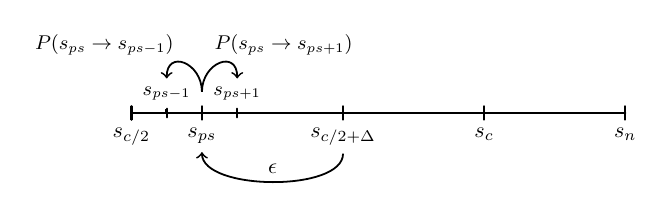
\begin{tikzpicture}[x=1.12cm, scale=0.8, every node/.append style={transform shape}]
    \draw[line width=0.2ex, line cap=round] (0,0) -- (7,0); %edit here for the axis
    \foreach \x in {0,1,3,5,7} % edit here for the vertical lines
    \draw[line width=0.2ex, line cap=round, shift={(\x,0)},color=black] (0pt,3pt) -- (0pt,-3pt);
    \foreach \x in {0.5,1.5} % edit here for the vertical lines
    \draw[line width=0.15ex, line cap=round, shift={(\x,0)},color=black] (0pt,2pt) -- (0pt,-2pt);
    \foreach \x/\y/\z in {
        0/$s_{c/2}$/a,
        1/$s_{ps}$/b,
        3/$s_{c/2+\Delta}$/c,
        5/$s_c$/d,
        7/$s_n$/e}
    \draw[line width=0.2ex, shift={(\x,0)},color=black] (0pt,0pt) -- (0pt,-3pt) node[below] (\z) {\y};
    \foreach \x/\y/\z in {
        0.5/\small$s_{ps-1}$/f,
        1//h,
        1.5/\small$s_{ps+1}$/g}
    \draw[line width=0.2ex, shift={(\x,0)},color=black] (0pt,0pt) -- (0pt,2pt) node[above] (\z) {\y};

    \begin{scope}[line width=0.15ex]
        %\path[->] (c) edge[out=-90, in=-85, looseness=0.7] node[above] {} (d);
        \path[->] (c) edge[out=-90, in=-90, looseness=0.7] node[above] {$\epsilon$} (b);
        \path[->] (h) edge[out=90, in=90, looseness=2] node[above,xshift=-0.5in] {\small$P(s_{ps} \to s_{ps-1})$} (f);
        \path[->] (h) edge[out=90, in=90, looseness=2] node[above,xshift=+0.4in] {\small$P(s_{ps} \to s_{ps+1})$} (g);
    \end{scope}
    %\draw [thick,decoration={brace,raise=1ex, amplitude=2ex},decorate] (5, 0) -- (7, 0) node[midway,above,yshift=3.5ex] {$b$};
\end{tikzpicture}


\caption{Representation of the space of feasible solutions. Outside the phase-shift point, the network builds a bias towards one end. At the $\Delta$ point, this bias is $\varepsilon$-irreversible.
% \Jon{I really didn't get the story here. It seems like cool graphical representations that would really help me understand the underlying arguments, but I missed something.}
}
\label{fig:states_feasible_solutions}
    \end{center}
\end{figure}

\noindent To ensure C1, we must find $\Delta$ such that the following condition holds:
\begin{equation}
\begin{split}
    \exists \Delta, \text{where}\ s_{c/2 + \Delta} &> s_{ps},\ s.t.\ \forall t \leq \phi:\\
    \varepsilon &\geq (V_c[s_{c/2 + \Delta}, s_{ps}])^t
\end{split}
\end{equation}
where $V_c$ is the $(c+1)^2$ probability transition matrix for the system.
In probability theory terminology, the statement above computes the $t$-step hitting probability, where the starting state is $s_{c/2 + \Delta}$ and the hitting state is $s_{ps}$.
Satisfying this first constraint, that is, moving the ensemble of nodes to a decision, is not sufficient. The nodes have to be able to assure \emph{themselves} that they can safely decide, which means they must ensure condition C2.
While there are multiple ways of constructing the predicate that ensures this condition, the one we adopt in Snowflake involves $\beta$ consecutive successful queries, such that $P(\textsc{isAccepted} \,|\, s_i \leq s_{c/2 + \Delta}) \leq \varepsilon$. 
To achieve this threshold probability of failure for C2, we solve for the smallest $\beta$ that meets inequality
$P(\mathcal{G}(\mathtt{p}, \phi/c) \geq \beta) \leq \varepsilon$
where $\mathtt{p} = P(\mathcal{H}_{\mathcal{N}, i}^k \geq \alpha k)$ and $\mathcal{G}(\mathtt{p}, \phi/c)$ is a random variable which counts the largest number of consecutive same-color successes for a run over $\phi/c$ trials.
Solving for the minimum $i$ yields $\beta$.

The task of the system designer, finally, is to derive values for $\alpha$ and $\beta$, given desired $n, b, k, \varepsilon$.
Choice of $\alpha$ immediately follows from $b$ and is $(n - b)/ n$, the maximum allowable size to tolerate $\leq b$ Byzantine nodes.
Solving for $\Delta$ with a closed form expression would be ideal but unfortunately is difficult, hence we employ a numerical, iterative search.
Since $k$ and $\beta$ are mutually dependent, a system designer will typically fix one and search for the other.
Because $\beta$ is a tunable parameter whose consideration is primarily latency vs.\ security, a designer can fix it at a desired value and search for a corresponding $k$.
Since low $k$ are desirable, we perform this by starting at $k=1$, and successively evaluating larger values of $k$ until a feasible solution is found.
Depending on $b$ and the chosen $\varepsilon$, such a solution may not exist. If so, this will be apparent during system design. 
% \Jon{I found myself afloat in a sea of single-letter variable names, and was wishing for a quick-reference key to decode them. (Or even better, for some to be eliminated. :V)}

We finalize our analysis by formally composing C1 and C2: 
\begin{theorem}
    If C1 and C2 are satisfied under appropriately chosen system parameters, then the probability that two nodes $u$ and $v$ decide on $\mathtt{R}$ and $\mathtt{B}$ respectively is strictly $< \varepsilon$ over all timesteps $0 \leq t \leq \phi$. 
\end{theorem}
\begin{proof}
    The proof follows in a straightforward manner from the core guarantees that C1 and C2 provide. Without loss of generality, suppose a single node $u$ decides $\mathtt{R}$ at time $t < \phi$, and suppose that the network is at state $s_j$ at the time of decision. By construction, $\textsc{isAccepted}$ will return true with probability no greater than $\varepsilon$ for all network states $s_i < s_{c/2 + \Delta}$. Therefore, since $u$ decided, it must be the case that $s_j > s_{c/2 + \Delta}$, whp. Lastly, since the system will only revert back to a state with a majority of $\mathtt{B}$ nodes with negligible probability once it is past $s_{c/2 + \Delta}$, the probability that a node $v$ decides on $\mathtt{B}$ is strictly $< \varepsilon$.
\end{proof}

For\ \ illustration purposes, we examine a network with $n = 2000,\ \alpha = 0.8$, $\varepsilon \leq 2^{-32}$, and throughput of 10000tps.
If we allow this system to run for \textasciitilde{}4,000 years (which corresponds to $\phi = 10^{15}$), we choose $\beta$ such that the probability of a node committing
at state $s_{c/2+\Delta - 1}$ is $< \varepsilon$.
A safety failure then occurs when both a node commits $\mathtt{R}$ and the system reverts to $\mathtt{B}$. Figure~\ref{figure:failure_theta_0} shows the probability of failure and the corresponding $\beta$ for different choices of $k$.

\begin{figure}[h!]
\tronly{\includegraphics[width=\linewidth]{figures/consecutive-beta-large.pdf}}
        {\includegraphics[width=\linewidth]{figures/consecutive-beta.pdf}}
    \caption{$\beta$ and failure probability $p_f$ vs. $k$ values (x-axis), with $n = 2000$, $\alpha = 0.8$.}
\label{figure:failure_theta_0}
\end{figure}

\begin{comment}
In this section, we have shown that if the network parameters chosen by the system designer satisfy both conditions C1 and C2, then probability of a safety failure in Snowflake is negligible. 
Finally, there exists one more consequence to the Snowflake protocol.
Namely,
\end{comment}
Note that a larger choice of the $\alpha$ parameter dictates a larger space of feasible solutions, which implies a larger tolerance of Byzantine presence. 
If the system designer chooses to allow a larger presence of Byzantine nodes, she may achieve this goal at the cost of liveness. 
%XXX expand on this counterintuitive idea at some point, it implies that we can put up with very large byzantine coalitions
%XXX how big can $b$ be?
%XXX KEVIN: There are actually many cool things I can be saying additionally here, but what is written up to now is sufficient for tech report. I will soon-enough add up some interesting insights about speed of convergence once the system actually enters s_{c/2 + \Delta}. 

\subsection{Safety Analysis of Snowball}\tronly{}{\vspace{-0.5em}}
In this section, we will demonstrate that Snowball provides strictly better
safety than Snowflake.
The key difference in protocol mechanics between Snowflake and Snowball is that correct nodes now monotonically increase their confidence in $\mathtt{R}$ and $\mathtt{B}$.
This limits the effect of random perturbations, as well as the impact of the Byzantine adversary.

To intuitively understand the behavioral differences between Snowball and its predecessor, we illustrate with an example, accompanied by some concrete numerical values.
\begin{comment}
The example will also provide intuition on how Snowball admits a safety guarantee strictly stronger than that of Snowflake. The goal of this section is to formally prove this guarantee.
\end{comment}
Suppose a network of size $n$ where $b = (1/5)n$, $\alpha = (4/5)k$ (i.e. the maximum allowable threshold to tolerate the $(1/5)n$ presence of Byzantine nodes), and where $k$ is chosen large enough to admit a feasible solution. 
Suppose that the network swings to state $s_{c/2 + \Delta}$, such that correct nodes have a non-negligible probability of deciding on $\mathtt{R}$, and suppose, for the sake of simplicity, that $\Delta$ is chosen as the highest possible value, specifically $c/2 + \Delta + b = \alpha n = (4/5)n$, the upper-threshold set up by the system designer. 

In this configuration, at least $(4/5)n - b = (3/5)n$ (correct) nodes prefer $\mathtt{R}$. 
These nodes perceive network support for $\mathtt{R}$ of at most $(4/5)n$ if the Byzantine nodes choose to also vote for $\mathtt{R}$, and at least $(3/5)n$ if the Byzantine nodes choose to withhold support for $\mathtt{R}$. 
Conversely, the rest of the $(1/5)n$ (correct) nodes that may prefer $\mathtt{B}$ perceive network support for $\mathtt{B}$ of at least $(1/5)n$ and at most $(2/5)n$, depending on the Byzantine strategy. 
Regardless of Byzantine strategy, however, all correct nodes that prefer $\mathtt{R}$ will have an expected growth of the $\mathtt{R}$ confidence to be strictly greater than the $\mathtt{B}$ confidence for the nodes that prefer $\mathtt{B}$. 
This is because network support for $\mathtt{R}$ is at least $(3/5)n$, which is greater than the maximum network support for $\mathtt{B}$ of $(2/5)n$. 
Therefore, once the network swings to the minimum required state, the expected growth of the $\mathtt{R}$-confidence will be greater than that of $\mathtt{B}$-confidence, for all correct nodes and for all Byzantine strategies. 

In the previous section, we provided the two conditions necessary for guaranteeing the safety of Snowflake. The second condition, C2, remains identical in Snowball, and therefore does not need to be modified and re-analyzed. Conversely, condition C1 (i.e. showing that the network is irreversible whp) needs to be re-analyzed. In this section, using the same intuition provided in the example above, we formally show how Snowball achieves irreversibility under strictly higher probability than in Snowflake. 

\tronly{
\paragraph{Security of Snowball.}
Figure~\ref{fig:snowball_simulator} illustrates the scheduler-based version of Snowball.
In Snowball, a node $u$ \textit{prefers} $\mathtt{R}$ if $u.d[\mathtt{R}] > u.d[\mathtt{B}]$, and vice versa. At the start of the protocol, these preferences are initialized to $\langle 0, 0 \rangle$. 
This is in contrast to Snowflake, where nodes prefer a color based only on the latest successful sample.
We can model the protocol with a Markov chain similar to that of Snowflake, and derive the parameters and feasibility for the protocol.

\begin{figure}[h!]
\begin{algorithmic}[1]
\State initialize $\forall u, u.\codecolor$
\State initialize $\forall u, u.\textrm{lastcol}$
\State initialize $\forall u, u.\codecount \coloneqq 0$
\State initialize $\forall u, \forall \codecolor' \in \{\texttt{R}, \texttt{B}\}, u.d[\codecolor'] \coloneqq 0$
\For{$t = 1$ to $\phi$}
    \State $u \coloneqq \Call{sample}{\mathcal{C}, 1}$
    \State $\mathcal{A}(u, \mathcal{C})$
    \State $\mathcal{K} \coloneqq \Call{sample}{\mathcal{N}\textbackslash u, k}$
    \State $P \coloneqq \texttt{[}v.\codecolor\quad\textbf{for}\ v \in \mathcal{K}\texttt{]}$
    \For{$c' \in \{\texttt{R}, \texttt{B}\}$}
    \If{$P.\Call{count}{\codecolor'} \ge \alpha\cdot k$}
        \State $u.d[\codecolor']\texttt{++}$
        \If {$u.d[\codecolor'] > u.d[\codecolor]$}
            \State $u.\codecolor \coloneqq \codecolor'$
        \EndIf
        \If{$\codecolor' \neq u.\textrm{lastcol}$}
            \State $u.\textrm{lastcol} \coloneqq \codecolor'$, $u.\codecount \coloneqq 0$
        \Else
            \State $\texttt{++}u.\codecount$
        \EndIf
    \EndIf
    \EndFor
\EndFor
\captionof{figure}{Snowball run by a global scheduler.}
\label{fig:snowball_simulator}
\end{algorithmic}
\end{figure}

We fix a $\Delta$ such that, under the Markovian construction of Snowflake, if the system reaches $s_{c/2 + \Delta}$, then whp it does not revert. We show that this choice of $\Delta$ provides an even stronger guarantee once the network switches protocol to Snowball.
Without loss of generality, we cluster the correct nodes into two groups, and represent each group through two nodes $u$ and $v$, where $u$ represents the set of correct nodes that prefer red and $v$ those that prefer blue. 
Lastly, let the state of the system be initialized at $s_{c/2 + \Delta}$.

% With non-negligible probability, $u$ will decide on $\mathtt{R}$, since the network is biased enough to trigger the decision predicate. 
The best possible confidence-configuration that the Byzantine nodes can attempt to force correct nodes into is where all $\mathtt{R}$-preferring nodes, represented by $u$, are forced to maintain nearly equal confidence between the two colors, and where all of the $\mathtt{B}$-preferring nodes, represented by $v$, gain as much confidence as possible for~$\mathtt{B}$. 

Let $u.d[\mathtt{R}] = u.d[\mathtt{B}] + 1$, corresponding to the minimal viable color difference for the red-preferring nodes, and let $v.d[\mathtt{B}] - v.d[\mathtt{R}] = \kappa$ be the difference for the blue-preferring nodes. While $\kappa \geq 0$, then the expectation of preference growths at time $t$ are:
\begin{equation}
    {\scriptsize
\begin{split}
    \mathbb{E}[{u.d}^t[\mathtt{R}]] &= \mathbb{E}[{u.d}^{t-1}[\mathtt{R}]] + \left(\frac{1}{2}+\frac{\Delta}{c}\right)P(\mathcal{H}_{\mathcal{N}, c/2 + \Delta + b}^k  \geq \alpha k)\\
    \mathbb{E}[{u.d}^t[\mathtt{B}]] &= \mathbb{E}[{u.d}^{t-1}[\mathtt{B}]] + \left(\frac{1}{2}+\frac{\Delta}{c}\right)P(\mathcal{H}_{\mathcal{N}, c/2 - \Delta + b}^k  \geq \alpha k)\\
    \mathbb{E}[{v.d}^t[\mathtt{R}]] &= \mathbb{E}[{v.d}^{t-1}[\mathtt{R}]] + \left(\frac{1}{2}-\frac{\Delta}{c}\right)P(\mathcal{H}_{\mathcal{N}, c/2 + \Delta}^k  \geq \alpha k)\\
    \mathbb{E}[{v.d}^t[\mathtt{B}]] &= \mathbb{E}[{v.d}^{t-1}[\mathtt{B}]] + \left(\frac{1}{2}-\frac{\Delta}{c}\right)P(\mathcal{H}_{\mathcal{N}, c/2 - \Delta + b}^k  \geq \alpha k)\\
\end{split}
    }
    \label{equation:expectation_snowball}
\end{equation}
Note that we are implicitly using an indicator function when adding up the probability of success to the expected confidence growth, where the expected value of the indicator value is exactly the probability of success of a sample. 
Substituting for Hoeffding's tail bound, we get the rate at which $\kappa$ decreases per time-step to be
\begin{equation}
    % p = \cfrac{c/2 + \Delta + b}{c+b}
    \begin{split}
    \small
        r = \biggl(\left(\frac{1}{2}-\frac{\Delta}{c}\right) &e^{-k\alpha \log \left(\alpha/\frac{c/2 - \Delta + b}{c+b}\right)}\\
    &e^{-k(1-\alpha) \log \left(\left(1-\alpha\right)/\left(1-\frac{c/2 - \Delta + b}{c+b}\right)\right)}\biggr)\\
        - \biggl(\left(\frac{1}{2}-\frac{\Delta}{c}\right)&e^{-k\alpha \log \left(\alpha/\frac{c/2 + \Delta + b}{c+b}\right)}\\
    &e^{-k(1-\alpha) \log \left(\left(1-\alpha\right)/\left(1-\frac{c/2 + \Delta + b}{c+b}\right)\right)}\biggr)\\
    \end{split}
    \label{equation:rate_decrease}
\end{equation}

Upon reaching $\kappa = -1$, the blue-preferring nodes will have flipped to red.
From then on, all correct nodes are red, and the confidence of red grows significantly faster than that of blue.
We now show that the rate of growth of $\mathtt{R}$ will always be larger than the rate of growth of $\mathtt{B}$, over all correct nodes. 

Letting $X({u.d}^t[\mathtt{R}])$ be a random variable that outputs the confidence of red for $u$ at timestep $t$, and letting $\bar X({u.d}^t[\mathtt{R}]) = X({u.d}^1[\mathtt{R}]) + \dots + X({u.d}^t[\mathtt{R}])$, we apply Hoeffding's concentration inequality to get that $P({\bar X({u.d}^t[\mathtt{R}])} - \mathbb{E}[\bar X({u.d}^t[\mathtt{R}])] \geq l) \leq e^{-2l^2t}$.
At time $t$, the expected confidence of red for $u$ is
\begin{equation}
    {u.d}^0[\mathtt{R}] + t\left(\frac{1}{2} + \frac{\Delta}{c}\right)\left(\frac{\frac{c}{2} + \Delta + b}{c+b}\right)
\end{equation}
And conversely the expected confidence of blue for $u$ is
\begin{equation}
    {u.d}^0[\mathtt{B}] + t\left(\frac{1}{2} + \frac{\Delta}{c}\right)\left(\frac{\frac{c}{2} - \Delta + b}{c+b}\right)
\end{equation}
Then, the probability that the expected value of red confidence is close to the expected value of the blue confidence is
\begin{equation}
    e^{-2t^3(1/2 + \Delta/c)^2(2\Delta/(c+b))^2}
    \label{equation:concentration_mean}
\end{equation}
Solving for $t$ that leads to such probability being negligible leads to:
\begin{equation}
    t = \left(\cfrac{\log(\varepsilon)}{-2\cdot(1/2 + \Delta/c)^2(2\Delta/(c+b))^2}\right)^{1/3}
    \label{equation:minimal_time}
\end{equation}
Therefore, at only a small number of timesteps $t$, $u$ has a red-confidence centered around its mean, with probability $\varepsilon$ close to the mean of the blue-confidence. An identical analysis follows for $v$.
In other words, after a small number of time-steps, the red-confidence of $u$ grows large enough such that the probability of this value being close to that of the blue-confidence is negligible. Further timesteps amplify this distance and further decrease the probability of the two confidences being close. 
}

\tronly{}{The details are provided in an accompanying technical report~\cite{avalanche}. The central result is as follows:}
We conclude our result with the following Theorem:
\begin{theorem}
Over all viable network parameters $n,\ b$, and for all appropriately chosen system parameters $k$ and $\alpha$, the probability of violating safety in Snowball is strictly less than the probability of violating safety in Snowflake.
\end{theorem}
\begin{proof}
%    The proof is straightforward.
Under the construction of Snowball in comparison to Snowflake, we see that safety criterion C2 remains the same. In other words, the consecutive-successes decision predicate has the same guarantees. 
On the other hand, the probabilistic guarantees of C1 change, meaning that the reversibility probabilities of the system are different. 
However, as we determined in Equation~\ref{equation:minimal_time}, over a few timesteps
$u$'s confidence difference between $\mathtt{R}$ and $\mathtt{B}$ grows large enough to guarantee that this confidence difference will revert back with only negligible probability.
As time progresses, the probability of being close decreases poly-exponentially, as shown in Equation \ref{equation:concentration_mean}. The same results follow for $v$, but inversely, meaning that the means get closer to each other rather than deviate. This continues until $v$ flips color. 
\end{proof}

\tronly{Snowball has strictly stronger security guarantees than Snowflake, which implies that appropriately chosen parameters chosen for Snowflake automatically apply for Snowball. Using the same techniques as before, the system designer chooses appropriate $k$ and $\beta$ values that ensure the desired $\varepsilon$ safety guarantees.}{}

% ------------------------------------------------------
% OLD STUFF ABOUT THETA 1 AND BYZANTINE OPTIMALITY ADDED
% TO FILE oldtheta1.tex, see line below. DO NOT DELETE!!
% % -------------
% DO NOT DELETE.
% DO NOT DELETE.
% DO NOT DELETE.
% -------------
Every correct node is chosen by the scheduler at most a fixed number of times, $\delta$, after which the value of every correct node is collected and counted.
Note another (and final) condition: if a node is selected and that node has seen $\phi$ consecutive majorities for the same value, it no longer updates its value, regardless of the output of the polling. 

\subsubsection{Safety of \Theta_1}
The expression for the hypergeometric experiment is reasonably complex, and it becomes hard to reason about the different ways that each of the variables inside the expression affects the outcomes. In particular, it is not clear how network size affects the experiment. This is of interest because if the effect of network size has little bearing on the outcomes of the experiment, it has important consequences for the scalability of the $\Theta_1$ protocol. To see how network size affects the system, we can fortunately make usage of the 

\subsubsection{Adversarial Optimality}
We will first try to determine the optimal strategy that the Byzantine
adversary can play.  Once we have this strategy, we will analyze how
effective this strategy is.
Recall that we do not care about violating liveness for conflicting
transactions, so the adversary's objective is to violate
safety, that is, it wants some correct node to decide red while another
correct node decides blue.  

As a thought experiment, consider that most correct nodes lean red
while only one correct node leans blue.  Given our sampling protocol,
it is clear that if there are not too many Byzantine nodes, the red-leaning
nodes will continue to lean red, while the blue-leaning node will
start increasing its confidence in red and eventually become red-leaning
as well.  It thus stand to reason that a primary objective of the adversary
is to have half of the correct nodes lean red, while the other half lean
blue, and to keep it this way.

However, the adversary faces a conflict.  Consider that the adversary
has only limited time ($\phi$ rounds) to accomplish its goal of
violating safety.  When half the nodes are leaning blue, and half
the nodes are leaning red, their confidence in either blue or red
will not grow rapidly, and they likely will not decide in the limited
amount of time.  Also, if some node $u$ is close to deciding blue
and a small majority of nodes are leaning blue, then if $u$ polls
a Byzantine node it is not clear whether the Byzantine node should
return red or blue.  If the Byzantine node returns blue, it may
cause $u$ to decide blue but still give the adversary a chance to
get other nodes to decide red.  If the Byzantine node returns red,
it may help restore the balance between red- and blue-leaning nodes.

This conflict for the adversary illustrates exactly the strength of
the Snowball protocol.  While it is relatively easy for the adversary
to prevent deciding on conflicting transactions, it is difficult for
the adversary to cause two correct nodes to decide different transactions.

\begin{comment}
If this is the situation, then if a correct
node samples other nodes, it will, by expectation, receive the same number of
red and blue votes from the correct nodes that it samples.

The Byzantine strategy then is straightforward:
if there are as many red-leaning nodes as blue-leaning nodes and
a red-leaning node samples from a Byzantine node, the Byzantine node
returns red, and vice versa.
If the node has equal confidence in red or blue, it does not matter
which color the Byzantine node returns and can, say, flip a coin.
If, however, the system is not in balance, and
there are more red than blue nodes, then a Byzantine node will always
``push back'' by returning blue (and vice versa).
We will later demonstrate that this strategy is optimal.

Next, we need to show that although optimal, the strategy cannot
cause a violation of safety with high probability.
We will show that whp no 
correct node ever decides (if there are conflicting values), and in particular
no two correct nodes ever disagree.
If the Byzantine strategy is non-optimal, correct nodes may decide, but
they will decide the same value whp.
\end{comment}

\begin{comment}
We define \emph{skew} as the maximum among the distances between the
confidence vectors (interpreted as points in a Euclidean space)
of correct node pairs.  For example, if there are three correct nodes
with confidence vectors $\langle 0, 3 \rangle$, $\langle 1, 3 \rangle$,
and $\langle 4, 0 \rangle$, then the skew is~5 (the distance between
the first and last confidence vector endpoints).
The optimal strategy for the Byzantine nodes is to maximize skew.

% TODO: Expand in sentences the notation written about maximal policy below. 
We want to characterize \textit{drift} in the differences of values between any two correct nodes. Specifically, letting the absolute difference between the values of any correct node correspond to some confidence differential, represented by $\max_{\Delta}(u) = u[0]-u[1]$ if $|u[0]| > u[1]$ and $\max_{\Delta}(u) = u[1]-u[0]$ if $u[1] > |u[0]|$, we desire to precisely quantify bounds on the maximum drifts between any two correct nodes, and for all possible execution instances $\mathcal{I}_i$. In other words, what is the execution path $\mathcal{I}_{opt}$ such that
\[
    \mathcal{I}_{opt}(\mathcal{C}^{t_0}) = \max_{\forall i}\{\mathcal{I}_i(\mathcal{C}^{t_0})\}
\]
where
\[
    \mathcal{I}_{i}(\mathcal{C}^{t_0}) = \max_{\forall u, v \in \mathcal{C}^{t_\phi}}\{\max_{\Delta}(u)-\max_{\Delta}(v)\}
\]
To exactly characterize the probability of a safety failure of the optimal execution path, we would need to calculate the probability distribution over all possible permutations of Byzantine answers, which is a function of the choices of execution of the correct nodes as well as the distribution of the choices of the neighbors.
In other words, over all possible execution paths (i.e. there are $c$ nodes to choose at each time step, for a total of $\phi^{c}$ ways of choosing over $\mathcal{C}$ nodes) and over all possible choices of the $k$-sampled neighbors (for a total of ${n \choose k}$ such choices, per node, per execution round), we would need to keep track of all of the possible tuples of the Byzantine value updates. 
Generating such a stochastic model would, plainly speaking, be infeasible. 
\end{comment}

\paragraph{Optimality Condition}
We can simplify the analysis greatly if we fix the Byzantine strategy to some optimal policy, $\mathcal{A}_{\pi}$. 
Let $s$ be a three-tuple where the first entry is a color configuration of the set of nodes in $\mathcal{C}$ (i.e. the set $\lbrace(u_1[\mathtt{R}], u_1[\mathtt{B}]), (u_2[\mathtt{R}], u_2[\mathtt{B}]), \dots, (u_c[\mathtt{R}], u_c[\mathtt{B}])\rbrace$, where $u[\mathtt{R}], u[\mathtt{B}] \in [0, \phi]$), the second entry is the chosen node at some round $u \in \mathcal{C}$ in round $t_i$, and the third entry is the round itself $t_i$. Let $\mathtt{S}$ be the set of all such tuples $s$. The elements of $\mathtt{S}$ are the necessary pieces of information needed for the Byzantine strategy. 
For each state $s \in \mathtt{S}$, the set of allowable actions for the Byzantine nodes is either $\mathtt{R}$ or $\mathtt{B}$. Let $P(s' | s, {\mathtt{R}})$ be the probability of transitioning from state $s$ to $s'$ given that the Byzantine strategy responds with $\mathtt{R}$, and conversely for $\mathtt{B}$. Let $\mathtt{Z}(s)$ be the reward for entering state $s$. Let the policy $\mathcal{A}_{opt}(s)$ be the optimal policy which returns the color chosen by the Byzantine node at state $s$, given round $i$. 
The utility $\mathcal{U}$ of $s$ (and the optimal policy) are then defined as
\begin{equation}
\begin{split}
\mathcal{U}(\mathcal{A}_{opt}, s) =\ \mathtt{Z}(s)\ +& \sum_{s' \in S} P(s' | s, \mathcal{A}_{opt}(s))\\
\times &\ \mathcal{U}(\mathcal{A}_{opt}, s')
\end{split}
\end{equation}
where 
\begin{equation}
\begin{split}
    \mathcal{A}_{opt}(s) &= \argmax_{a \in \lbrace \mathtt{R}, \mathtt{B} \rbrace} \left \lbrace \sum_{s' \in S}P(s'|s, a)\mathcal{U}(\mathcal{A}_{opt}, s') \right \rbrace
\end{split}
\end{equation}
These are the equations that follow from Bellman's optimality principle. Note that we do not include a discount factor. Further, we assign a reward of 1 to the states where there exists two nodes $u, v$ such that $\gamma_u \geq \gamma$ and $\gamma_v \leq 1/\gamma$. 

Since the state space is computationally infeasible, we solve for the optimal policy inductively, rather than iteratively. 
Let $count(\mathcal{C}^{t_i}, \mathtt{R})$ be defined as: 
\begin{equation}
\begin{split}
    count(\mathcal{C}^{t_i}, \mathtt{R}) = \sum_{u \in \mathcal{C}^{t_i}} \mathbbm{1}(u, \mathtt{R})
\end{split}
\end{equation}
where $\mathbbm{1}$ is the indicator function defined as:
\begin{equation}
\begin{cases}
    \mathbbm{1}(u, \mathtt{R}) = 1\ \text{\textbf{if}}\ u[\mathtt{R}] > u[\mathtt{B}]\\
    \mathbbm{1}(u, \mathtt{R}) = 0\ \text{\textbf{if}}\ u[\mathtt{R}] < u[\mathtt{B}]\\
    \mathbbm{1}(u, \mathtt{R}) = \{1, 0\}\ \text{\textbf{if}}\ u[\mathtt{R}] == u[\mathtt{B}]\ \text{\textbf{and} $u$ lastly}\\
    \text{preferred $\{\mathtt{R}, \mathtt{B}\}$}
\end{cases}
\end{equation}
and conversely for $count(t_i, \mathtt{B})$. 

Let $\mathcal{C}_{\mathtt{R}}$ be the set of correct nodes that the Byzantine nodes color as red at the cold start phase, and $\mathcal{C}_\mathtt{R}$ the converse. It is easy to see that a coloring of equal split between red and blue in the cold-start phase is the optimal configuration for a single iteration of the $\Theta_1$ protocol. It is not clear, however, how this configuration must evolve (if at all) as time progresses. 

Let $\mathcal{A}_\pi$ be the chosen Byzantine strategy described formally in Figure \ref{figure:mathcal_a_pi}. 
\begin{figure}[h!]
\label{figure:mathcal_a_pi}
\fbox{
    \parbox{0.95\linewidth}{
        \begin{center}
            \textbf{The $\mathcal{A}_\pi$ policy}
        \end{center}
        Let the Byzantine nodes set $\mathcal{C}_\mathtt{R}$ to be exactly half of the correct nodes in the network, and $\mathcal{C}_\mathtt{B}$ the other half at the cold-start phase. We initialize a local memory $\mathds{M}$, which stores various information about the history of execution up to step $t_i$. Let $\{\mathcal{C}', u, t_i\} \leftarrow s$, where $\mathcal{C}^{t_i} = \mathcal{C}'$ (note that there are multiple valid versions of $\mathcal{C}^{t_i}$, nevertheless in this case we refer to the specific set $\mathcal{C}$ extracted from state $s$). 
        \begin{itemize}
            \item If $count(\mathcal{C}^{t_i}, \mathtt{R}) = c/2$:
            \subitem In this case, the set of correct nodes is equally split. If $u \in \mathcal{C}_\mathtt{R}$, then all Byzantine nodes are colored red. Conversely for blue. Add $s$ to $\mathds{M}$, and return. 
            \item If $count(\mathcal{C}^{t_i}, \mathtt{R}) < c/2$:
            \subitem In this state, the set of correct nodes has shifted to a majority blue. This implies that at some time step $t_j < t_i$, a node $v \in \mathcal{C}_\mathtt{R}$ gained at least 1 extra confidence for blue than for red. Locate this node $v$ by searching the history stored in memory $\mathds{M}$. Move $v$ to the corresponding color assignment, i.e. set $\mathcal{C}_\mathtt{R} = \mathcal{C}_\mathtt{R}\backslash v$ and $\mathcal{C}_\mathtt{B} = \mathcal{C}_\mathtt{B} \cup v$. Search in $\mathcal{C}^{t_i}$ for all nodes $v'$, s.t. $\mathbbm{1}(v', \mathtt{B}) = 1$, and find the $v'$ with the minimum skew between blue and red, i.e. $\min \{v'[\mathtt{B}] - v'[\mathtt{B}]\} \forall v'$. Move the target $v'$ to the opposite color assignment, i.e. set $\mathcal{C}_\mathtt{B} = \mathcal{C}_\mathtt{B}\backslash v'$ and $\mathcal{C}_\mathtt{R} = \mathcal{C}_\mathtt{R} \cup v'$. Finally, if $u \in \mathcal{C}_\mathtt{R}$, then all Byzantine nodes are colored red. Conversely for blue. Add $s$ to $\mathds{M}$, and return. 
        \end{itemize}
    }
}
\end{figure}

\begin{comment}
    \begin{algorithm}
    \begin{algorithmic}[1]
    \Procedure{$\mathcal{A}_\pi$}{$s$}
    \State $\{\mathcal{C}', u, t_i\} \leftarrow s$
    \If{$\mathbbm{1}(u, \mathtt{R})$} \Comment{$u$ prefers $\mathtt{R}$}
    \If{$u \in \mathcal{C}_\mathtt{R}$}
    \State
    \EndIf
    \EndIf
    \State $\mathcal{A}(u, \mathcal{C})$ \Comment{Deterministic Byzantine strategy}
    \State $s \xleftarrow{\$^k} \mathcal{N}$\textbackslash $u$
    \If{count($s, \mathtt{R}$) $\geq$ $\alpha k$}
    \State $u[\mathtt{R}]~ += 1$
    \EndIf
    \If{count($s, \mathtt{B}$) $\geq$ $\alpha k$}
    \State $u[\mathtt{B}]~ += 1$
    \EndIf
    \State update($\mathcal{C}$, $u$)
    \EndProcedure
    \end{algorithmic}
    \end{algorithm}
\end{comment}

\begin{theorem}
The Byzantine strategy $\mathcal{A}_\pi$ is optimal, i.e. $\mathcal{A}_\pi = \mathcal{A}_{opt}$.
\end{theorem}
\begin{proof}
We inductively prove the claim. 
The base case is when the nodes are equally split in half, i.e. $count(\mathcal{C}^{t_i}, \mathtt{R}) = c/2$. Let $\mathcal{H}_{\mathcal{N}, c/2 + b + j}^k/\mathcal{H}_{\mathcal{N}, c/2 - j}^k$ represent the expected ratio growth of $\gamma_u$, where $u \in \mathcal{C}^\mathtt{R}$. 
Naturally, this ratio grows as $j$ grows (i.e. as the number of red-preferring correct nodes increases). 
However, the converse is also true, meaning that as $j$ increases, the $\gamma_v$ ratio for $v \in \mathcal{C}_\mathtt{B}$ decreases at the same rate. 
In particular, this rate is poly-exponential, meaning that even small changes to $j$ incur large benefits (and conversely penalties) on the confidence ratios. 
Therefore, the optimal split between correct nodes that maximizes the probability of $\gamma_u > \gamma_v$ and $\gamma_v > 1/\gamma$ where $u$ prefers red and $v$ prefers blue is when $j = 0$. 
In the usual case, the Byzantine nodes initially label the correct nodes equally between red and blue, and respond with red whenever a red-labelled correct node samples, and blue whenever a blue-labelled correct node samples. 
However, in the case when an initially red-labelled node (i.e. $u \in \mathcal{C}_\mathtt{R}$) suddenly switches confidence to blue, the Byzantine node must update it's strategy. 
The Byzantine nodes have three options: either keep responding red to the newly switched node, update responses to blue, or choose a new node and update its colors. 
Since every selection by the scheduler is uniformly at random, the expected number of times a node will be selected starting from time $t_i$ is equal amongst all correct nodes and is exactly $\phi - i / c - 1$. 
Therefore, in expectation, there is no difference between $u$ and a node $v$ which prefers the same color and which has no bigger skew than $u$. 
Sticking to the prior color labelling is clearly suboptimal since the growth of $\gamma_*$ of the new majority color will be larger than the minority color. Therefore, the optimal strategy is to simply pick the node of same color as the newly flipped node that has the \textit{minimum} skew (i.e. confidence) in its color. 
\end{proof}

Under no adversarial presence, the progress made by correct nodes is equal, in expectation, amongst all honest nodes. More formally, let $\mathcal{B} = \emptyset$. Then, $\forall u^{t_i}, v^{t_i} \in \mathcal{C}^{t_i}$, $i \geq 0$, 
\[
    \mathbb{E}[u^{t_i}[\mathtt{R}]] = \mathbb{E}[v^{t_i}[\mathtt{R}]]
\]
\[
    \mathbb{E}[u^{t_i}[\mathtt{B}]] = \mathbb{E}[v^{t_i}[\mathtt{B}]]
\]
At any time-step, the probability of each correct node being selected and subsequently adding either a red ball or blue ball is a function of the underlying number of red and blue preferences, but otherwise equal and uniform among all nodes. In Lemma \ref{lemma:expected_absorption}, we computed the expected number of steps to reach the state where all nodes prefer red. Upon reaching this state, every new added color will be the same, and growth of the opposing color will be zero. 

If Byzantine nodes are introduced, the expectation changes as a function of the underlying Byzantine strategy. Let $p_q^l(\mathtt{R}, \mathcal{S}, k, \alpha)$ be the probability of achieving at least $l$ consecutive successes for the color red over a sequence of $q$ trials given that $\mathcal{S}$ nodes in the network $\mathcal{N}$ prefer red. We let $\epsilon < 1$ be a security parameter, and after fixing $q$, we solve for the minimal value of $l$ such that 
\[
    p_q^l(\mathtt{R}, c, k, \alpha) \leq \epsilon
\]
In other words, we compute the minimal number of consecutive support for red until, with probability no more than $\epsilon$, at least $c$ nodes in the network also prefer red. 

It is easy to see that the probability is equal between the opposing colors as well as maximal when $\mathcal{S} = c/2 + b$. However, this probability is clearly much smaller than $\mathcal{O}(\epsilon^2)$. Suppose that the Byzantine nodes deviate from the optimal strategy in order to render the probability of committing at least one color to some value greater than $\epsilon$. In that case, the Byzantine nodes must allow the correct nodes to swing away from an equal network split. 

At this point in the deviation of the strategy, the ``snowball'' effect of $\Theta_1$ becomes apparent and highly compounded. Let $c/2 + \delta$ represent the expansion of the number of correct nodes towards red, and $c/2 - \delta$ the contraction of the number of correct nodes towards blue. Using the result from a prior lemma, the ratio of the speed of absorption will now be $g(c/2 + \delta)$. 

\begin{comment}
========= END PHASE 1

Fortunately, we can make usage of a useful observation: the probability of two independent successes for \texttt{opposing} values for any pair of hypergeometric experiments is maximum only when the frequency of the values in the network is exactly equal. 
To prove this, we simply need to solve for $i$ in the following expression: 

\begin{equation}
\max \{P(\mathcal{H}_{n, i}^k \geq \alpha k)*P(\mathcal{H}_{\mathcal{N}, n-i}^k \geq \alpha k)\}, 0 \geq i \geq n
\end{equation}

This probability is increases exponentially quickly as $i \rightarrow n/2$, with a maximum at $n/2$, and an exponential dropoff from $i = n/2$ to $n$. 
This observation is tremendously helpful because it allows us to fix the Byzantine adversary to a single optimal strategy: force the correct nodes into two equally split partitions, and -- throughout all $\delta$ executions -- put all the Byzantine nodes towards answering the corresponding value to each partition. 
Any other split, including non-fixed dynamic Byzantine strategies, would incur lower probability of success. 

Following on our observation, we can now fix the Byzantine strategy to the following: at time $t_0$, the Byzantine nodes choose two equal partitions of correct nodes, and for each subsequent time step, every Byzantine node will answer $1$ whenever the first partition queries and $2$ whenever the second partition queries. 

The probability that we receive $\phi$ or more successes over $\delta$ trials is a complicated expression, whose exact value requires a recursive expression. We leave the reader to Feller\cite{feller1} (Vol 1. Sec. XIII.7) for more information. Let $\mathcal{U}_{\delta}(\mathcal{H}_{\mathcal{N}, C^{t_i}}^k)$ be the random variable that outputs the number of consecutive successes of the hypergeometric experiment over $\delta$ trials. 
Then, the probability that a specific correct node receives $\phi$ or more consecutive successes is then: 

\begin{equation}
P_{consecutive} = \frac{1}{|\mathcal{C}|}P(\mathcal{U}_{\delta}(\mathcal{H}_{\mathcal{N}, C^{t_i}}^k) \geq \phi)
\end{equation}

The probabilities are symmetric across all correct nodes. Therefore, the probability of safety failure ($P_{sf}$) over all possible $|\mathcal{C}/2|^2$ pairs of correct nodes is then: 

\begin{equation}
    P_{sf} = |\mathcal{C}/2|^2 * P_{consecutive}^2
\end{equation}

The probabilities of safety failure are shown in Figure \ref{fig:safety_failure}.

\begin{figure}[h!]
\centering
\includegraphics[width=\linewidth]{./figures/safety_failure.pdf}
\caption{Probability of safety failure, $\phi = 20$, $\delta = 100$, $|\mathcal{N}| = 500$, and $k = 10$, for various size of Byzantine nodes and $\alpha k$.}
\label{fig:safety_failure}
\end{figure}

% \subsubsection{Liveness of \Theta_1}
% A key metric related to liveness is convergence latency, the amount of time between the introduction of a value proposal to the time every correct node agress on the same value.
% Described in terms of network configurations, this convergence latency calculates the expected number of rounds from any bivalent network configuration until reaching a state where all correct nodes vote for the same value. 
% We first show that convergence latency for a Byzantine-free network is logarithmic in the size of the network. Later, we calculate bounds on the maximum adversarial size that still guarantees expected logarithmic convergence. 
% Let the system be initialized to state $\psi = \{|\mathcal{C}_1^{t_0}|, |\mathcal{C}_2^{t_0}|\}$. 
% We perform a Markovian analysis on the probabilities of transitioning to any of all the possible states arising from $\psi$. 
% The state space $\mathbb{S}$ of all possible configurations arising from $\psi$ is all possible bivalent network splits between values $1$ and $2$, such that $|\mathcal{C}_1^{t_0}| + |\mathcal{C}_2^{t_0}| = |\mathcal{N}|$. 
% As an example, suppose the total number of correct nodes is 100. Then, all possible states of the system are $\{0, 100\}, \{1, 99\}, \dots, \{100, 0\}$.
% We can now construct the transition probability matrix $M$ of size $|\mathbb{S}| \times |\mathbb{S}|$. The expression for generating the values inside $M$ is highly verbose, however to provide the reader some intuition on how it is build, we given an example. Suppose the system is at state $\{50, 50\}$. Then, the system can only move to states $\{49, 51\}$, $\{51, 49\}$, or itself. The probability of moving to $\{49, 51\}$ is the probability of selecting a node that votes value $2$ and having that node switch to value $1$. The probability of staying in place is the probability that any selected node does not achieve the required $\alpha k$ threshold, or it achieves a threshold for its own value. $M$ will be sparse since most states will have only a transition to a small number of states.

% Given any starting state $s \in \mathbb{S}$, the hitting time $\mu$ is the expected number of transitions to reach states $A = \{\{0, |C|\}, \{|C|, 0\}\}$. 
% To calculate the hitting time, we first construct the system of linear equations shown in equation \ref{equation:minimalsolution} for all states in $\mathbb{S}$.

% \begin{equation}
% \label{equation:minimalsolution}
% \begin{cases}
% \mu_{sA} = 0, & \forall s \in A\\
% \mu_{sA} = 1 +\sum_{r\notin A}^{}{p_{sr}\mu_{rA}}, & \forall s \notin A
% \end{cases}
% \end{equation}

% The minimal non-negative solution vector $\mu_{A}~=~(\mu_{sA}, s \in \mathbb{S})$ to the system of linear equations in equation \ref{equation:minimalsolution}, yields the expected number of rounds to reach one of the convergence states. In other words, the solution gives the expected number of rounds for each node before all nodes agree on the same value.

% The convergence latency grows logarithmically with the network size, as shown in Table \ref{table:growth_worst_case}. 
% At 10k nodes, for example, the equal-network split expected time to converge is around 10 rounds. 
% \begin{table}[h!]
% 	\centering
% 	\begin{tabular}{llllll}
% 		Net. Size   & 600    & 1200   & 2400   & 4800   & 9600    \\ \hline
% 		Exp. Conv. & 7.18 & 7.94 & 8.69 & 9.44 & 10.19
% 	\end{tabular}
% 	\caption{Expected number of per-node-iterations to convergence starting at worst-case (equal) network split. Network sizes grow exponentially, whereas worst-case convergence grows logarithmically. $k = 10,\ \alpha=6$.}
% 	\label{table:growth_worst_case}
% \end{table}

\paragraph{Adversarial Progress} 
Without loss of generality, let $\lambda$ be chosen such that the expected frequency of $v_1$ and $v_2$ amongst the $\lambda$ chosen neighbors is nearly the same as $cn(v_1)$ and $cn_(v_2)$. 
In order to prevent progress, the number of adversarial nodes must then be larger than the absolute difference between the total number of honest nodes that vote for $v_1$ and $v_2$. This absolute difference denotes the total number of nodes that the adversary must have in its control in order to maintain an equal split between honest nodes. This adversarial size denotes the minimal adversarial size to prevent convergence in expected logarithmic number of rounds. 

Conversely, we can look at the case when the adversary pushes honest nodes to commit one value, and then equivocates. In this case, As long as the adversary is greater than ($1 - \beta/\lambda$), honest nodes that have not yet committed will no longer be able to commit. Any and all solicitations from any honest node will result in expected $(\lambda-\beta)/\lambda$ or more equivocations, which is insufficient to make progress.

\label{section:analysis}
\subsection{Snowball Safety Analysis}
% \label{subsec:safetyanalysis}
% \subsubsection{Terminology and Definitions}
% \label{subsubsec:termanddef}
% In this subsection, we refresh the reader of some of the old notations and as well introduce new notation, terminology, and definitions. 
%Finally, let $T_i$ and $T_j$ be two conflicting transactions belonging to the same conflict set. 

In order to analyze the safety of our protocol, we turn our focus exclusively towards two transactions of interest, $T_i$ and $T_j$, which belong to the same conflict set. 
Although the system is comprised of many conflicting transactions, we can safely ignore transactions that are not in the ancestry or progeny sub-graph of $T_i$ and $T_j$, since -- by construction -- those transactions are completely independent from $T_i$ and $T_j$ and thus do not contribute to the evolution of preference for either of the transactions of interest. 
Lastly, we note that unless explicitly stated, the analysis is through a ``God's eye'' view of the network. 

In the specification section (S. \ref{subsection:specification}), we introduced the general definition of \textit{preference} for a transaction $T$. 
Using that definition, we construct the notion of \textit{network support} for $T$, denoted as $\mathcal{S}_{u}^{t}(T)$, which represents the fraction of nodes in $\mathcal{N}$ that prefer $T$ at time $t$ as perceived by node $u$. 
To illustrate, suppose that the correct nodes are equally split in preference between $T_i$ and $T_j$. Furthermore, let $\mathcal{B}_{u}^{t}(T_i), \mathcal{B}_{u}^{t}(T_j) \subseteq \mathcal{B}$, be the subsets of the Byzantine nodes that vote $T_i$ and $T_j$ respectively as perceived by node $u$, which are mutually exclusive since according to $u$'s perspective the same Byzantine node cannot prefer two equivocating transactions simultaneously. 
A correct node $u$ would then observe that the network support for $T_{\{i,j\}}$ must be $\mathcal{S}_{u}^{t}(T_{\{i,j\}}) = (|\mathcal{B}_{T_{\{i,j\}}}| + |\mathcal{C}|/2)/|\mathcal{N}|$). 

Lastly, we call a \textit{solicitation} the act of $u$ querying a set of $k$ neighbors, chosen uniformly at random, to discover if they prefer transaction $T_i$. 
Note that necessarily $k \leq |\mathcal{N}|$, but otherwise the choice of size of $k$ is independent of the size of $\mathcal{N}$, as discussed previously.

% \subsubsection{Network Model}
\paragraph{Network Model}
We initially assume that every node has full view of every other node. 
Later, we relax this requirement to allow for looser views. 
Each node maintains a logical round counter (time) that starts at 0 at its initial solicitation and is incremented by one for each solicitation of a child transaction. 
Importantly, we remind that there is no notion of global system rounds, unless explicitly stated.

For simplicity, we assume that each node receives all $k$ responses of a solicitation within the same round. 
Later, we relax this requirement to interleave solicitation responses. 

% \subsubsection{Byzantine Adversary}
% \label{subsec:byzantineadversary}
\paragraph{Byzantine Adversary}
The adversary, whose nodes are in set $\mathcal{B}$, is round-adaptive and can both read all messages and view the state of all nodes in the network.
Round-adaptive means that the adversary can choose a new strategy for each of its nodes after seeing the messages exchanged by correct nodes.
In other words, whenever a correct node solicits its neighbors, the adversary can correspondingly instruct nodes under its ownership before the correct node has the chance to receive any responses. 
Such an adversary is only prohibited from modifying the internal state of a correct node and the in-transit responses between any two correct nodes. 

\subsubsection{Analysis}
\label{subsec:analysis}
% \paragraph{Statistical Errors and Parameters}
% We begin the analysis by first extracting some statistical bounds on protocol parameters. 
% We extract these bounds by isolating a single correct node $u$, and analyzing the results of a single isolated network polling experiment. Basically, we freeze the network at some specific point in time $t$ and then compute the statistical errors between two nodes $u$ and $v$. 

% For notational ease, we represent $\mathcal{S}_{u}^{t}(T_i)$ as $\mathcal{S}'$. 
% Let $\mathcal{H}_{N, \mathcal{S}'}^k \rightarrow [0, k] \in \mathbb{N}$ be a random variable which represents the total count of the $k$ randomly chosen neighbors that prefer transaction $T_i$ at round $t$ as queried by $u$. $\mathcal{H}$ is parameterized by the sample size $k$, the network $\mathcal{N}$, and the network support of $T_i$, $\mathcal{S}'$. For some constant $1/2 \leq \alpha \leq 1$, we are interested in the probability that a majority or more, $\alpha k \in \mathbb{N}$, of the sampled $k$ neighbors prefer $T_i$. The probability can be calculated as follows, 
% \begin{equation}
% P(\mathcal{H}_{\mathcal{N}, \mathcal{S}'}^k \geq \alpha k) = \sum_{j = \alpha k}^{k} \frac{{\mathcal{S}'|\mathcal{N}| \choose j}{|\mathcal{N}| - \mathcal{S}'|\mathcal{N}| \choose k - j}}{{|\mathcal{N}| \choose k}}
% \label{eq:hypergeometric}
% \end{equation}
% where the expected value of $\mathcal{H}_{\mathcal{N}, \mathcal{S}'}^k$ is exactly $k\mathcal{S}'$. From now on, if $\mathcal{H}_{N, \mathcal{S}'}^k \geq \alpha k$, we say that the solicitation was successful. 
% %Intuitively, the meaning behind this term is that some threshold majority $\alpha k$ of the solicited neighbors indeed support the transaction in question.

% We use the Hoeffding \cite{hoeffding1963probability} inequality to calculate the probabilities of deviation from the expected result of the polling experiment. Hoeffding's tail bounds then show that -- given a fixed constant $\psi$ -- the probability $\mathcal{H}$ deviating by $\psi$ from the expected value is given by, 
% \begin{equation}
% \begin{split}
%     P(\mathcal{H}_{N, \mathcal{S}'}^k \leq (\mathcal{S}'-\psi)k) %&\leq e^{-k\mathcal{D}(\mathcal{S}'-\psi, \mathcal{S}')} %\\
%     %&
%     \leq e^{-2\psi^2k}
% \end{split}
% \end{equation}
% % where $\mathcal{D}(\mathcal{S}'-\psi, \mathcal{S}')$ is the Kullback-Leibler divergence, measured as
% % \begin{equation}
% % \begin{split}
% %     \mathcal{D}(\mathcal{S}'-\psi, \mathcal{S}') &= (\mathcal{S}'-\psi) \log (\frac{\mathcal{S}'-\psi}{\mathcal{S}'}) \\
% %     &+ (1 - \mathcal{S}' + \psi) \log \frac{1 - \mathcal{S}' + \psi}{1 - \mathcal{S}'}
% % \end{split}
% % \end{equation}
% The very first thing to notice is that the probabilities are independent of network size, meaning that network size doesn't affect the performance of the protocol. 

% The second thing to notice is that the the upper bound $e^{-2\psi^2k}$ indicates that the probability of success of a solicitation is an inverse exponential parametrized by the sample size $k$. 
% For $k$, every +1 increase means an \textit{exponential decrease} in network view error.

% The third and last thing to notice is the implication for the value $\psi$, which has a quadratic effect on the exponential decrease in network view error. The network split amongst the correct nodes that maximizes the tail bound probability is exactly when half of the correct nodes are partitioned to initially prefer $T_i$ and half to initially prefer $T_j$. If the Byzantine nodes partition the network at some other ratio, the probability the Byzantine adversary successfully forces $u$ to prefer $T_i$ and $v$ to prefer $T_j$ for one solicitation is suboptimal. However, although this conclusion is correct over a single polling experiment, it may not hold over multiple experiments. This is because it would need to account for changes in the underlying graph structure. To that end, we now begin to analyze the protocol as it evolves over time. 

% % The implication of this result is that the optimal strategy for the Byzantine nodes is to minimize the deviation of $\psi$ (i.e. $\psi, k \rightarrow 0$), by splitting the network equally into two conflicting halves. 

% %The structure of the dag confers an important property. 
% %Due to the invariant imposed by the structure of the dag which states that every transaction on the path to a preferred child must be preferred in turn, every successful solicitation of a transaction implies a successful solicitation of its parent. 
% % Let $T' \xleftarrow{*} T$. At any time $t$, we necessarily have 
% % \begin{equation}
% % P(\mathcal{H}_{N, \mathcal{S}_{u}^{t}(T')}^k \geq \alpha k) \geq P(\mathcal{H}_{N, \mathcal{S}_{u}^{t}(T)}^k \geq \alpha k)
% % \end{equation}
% % We can now substitute the net total solicitations of the child transactions with an equivalent set of repeated solicitations for the parent transaction. 
% % This simplification allows us to focus solely on $T_i$, and safely ignore all other transactions except direct ancestors of $T_i$. 

% % Let $\mathcal{P}_b$ = $\{T_i, T_j\}$ be a set of two conflicting transactions. 
% % Let $u, v \in \mathcal{C}$ be any two correct nodes, and let $c_{\{u, v\}}(T_{\{i,j\}}, n)$ represent the confidence (i.e. the number of successful solicitations) for each of the transactions by each of the two correct nodes after sampling $n$ children transactions at rounds $t_0, t_1, \dots, t_n$, respectively. 

% % The expectation of the confidence of transaction $T_i$ after $n$ solicitations is equal to the probability of a successful solicitation for $T_i$ summed independently over every one of the $n$ experiments. More precisely, 
% % \begin{equation}
% % \begin{split}
% %     \mathbb{E}[c_{u}(T_{i}, n)] &=\ \sum_{j = 0}^{n}P(\mathcal{H}_{N, \mathcal{S}_{u}^{t_j}(T_i)}^k \geq \alpha k) \\
% % \end{split}
% % \end{equation}
\paragraph{Evolution Over Time}
The Byzantine nodes have the freedom to attack the system using any strategy. 
In order to maximize damage, the Byzantine nodes must pick the path of execution that ensures that the confidence of the two equivocating transactions is maximized between two correct nodes.
The adversary has access to a large set of attack options. On the one extreme end, the adversary may launch a ``bifurcation attack'', where the attacker equivocates at the very beginning and attempts to split the network equally in half, hoping that part of the network slowly prefers one transaction and the other half prefers the other. On the other extreme end, the adversary can launch a ``double-spend'' attack, where the adversary behaves correctly at the beginning, but after some large amount of time equivocates. 

% To calculate these expectations, and consequently define the most damaging Byzantine strategy, we must first extract some tail bounds on $\mathcal{H}$. 
%Figure \ref{fig:hypersplits} shows the probability of a single successful experiment over various network splits. 
%The probability of a single successful iteration decreases poly-exponentially with increasing difference between $\mathcal{S}N$ and $\alpha k$. 
% The most relevant tail bound can be extracted from Hoeffding \cite{hoeffding1963probability}. Given a network support $\mathcal{S}'$, the expected value of $\mathcal{H}_{N, \mathcal{S}'}^k$ is exactly $k \mathcal{S}'$. Hoeffding's inequality then shows that -- given a fixed constant $\psi$ -- the probability $\mathcal{H}$ deviating by $\psi$ from the expected value is given by, 
% \begin{equation}
% \begin{split}
%     P(\mathcal{H}_{N, \mathcal{S}'}^k \leq (\mathcal{S}'-\psi)k) %&\leq e^{-k\mathcal{D}(\mathcal{S}'-\psi, \mathcal{S}')} %\\
%     %&
%     \leq e^{-2\psi^2k}
% \end{split}
% \end{equation}
% % where $\mathcal{D}(\mathcal{S}'-\psi, \mathcal{S}')$ is the Kullback-Leibler divergence, measured as
% % \begin{equation}
% % \begin{split}
% %     \mathcal{D}(\mathcal{S}'-\psi, \mathcal{S}') &= (\mathcal{S}'-\psi) \log (\frac{\mathcal{S}'-\psi}{\mathcal{S}'}) \\
% %     &+ (1 - \mathcal{S}' + \psi) \log \frac{1 - \mathcal{S}' + \psi}{1 - \mathcal{S}'}
% % \end{split}
% % \end{equation}
% The very first thing to notice is that the probabilities are independent of network size, and are only a function of the sampled neighbor size $k$. This means that the network size doesn't affect performance of the protocol.

% The second thing to notice is that the the upper bound $e^{-2\psi^2k}$ indicates that the probability of success of a solicitation is an inverse exponential parametrized by the squared value of $\psi$. 
% The implication of this result is that the optimal strategy for the Byzantine nodes is to minimize the deviation of $\psi$ (i.e. $\psi, k \rightarrow 0$), by splitting the network equally into two conflicting halves. 
%Correct nodes can be fooled by Byzantine nodes by tuning parameters such that $e^{-2\psi^2k}$ is maximized. 
%This occurs when the deviation and sample size approach zero (i.e. $\psi, k \rightarrow 0$). 
% Since the Byzantine nodes are limited in their network presence, the most damaging strategy must necessarily be when all correct nodes are equally split. 

We start calculating the evolution of confidence between $T_i$ and $T_j$ by first computing the network split between the two transactions without introducing any children transactions. Let $T_*$.\texttt{sum} be the total sum of all chits for transaction $T_*$ amongst all correct nodes in the network. Let $\mathcal{C}_1$ be the subset of correct nodes that prefer $T_i$ at time $t = 0$, and $\mathcal{C}_2$ the corresponding set for $T_j$. Lastly, let $\mathcal{Z}_1$ be the subset of correct nodes that the Byzantine nodes have chosen to force to prefer $T_i$, and $\mathcal{Z}_2$ be the corresponding set of nodes for $T_j$. At $t = 1$ (the base case), the we can compute the new values of $T_*$.\texttt{sum} as follows:

\begin{equation}
    \begin{split}
        & T_1.\text{\texttt{sum}} = 0;\ T_2.\text{\texttt{sum}} = 0;\\
        t_1:\ \ \ &\gamma_{1}^{t_1} \leftarrow \frac{\mathcal{Z}_1}{\mathcal{C}} P(\mathcal{H}(\mathcal{N}, \mathcal{C}_1 + \mathcal{B}, k, \alpha) \geq \alpha k)
        % = \sum_{i = \alpha}^{k} {k \choose i}\bigg(\frac{\mathcal{C}_1 + \mathcal{B}}{\mathcal{N}}\bigg)^i \bigg(1 - \frac{\mathcal{C}_1 + \mathcal{B}}{\mathcal{N}}\bigg)^{k - i}
        \\
        & \gamma_{2}^{t_1} \leftarrow \frac{\mathcal{Z}_2}{\mathcal{C}} P(\mathcal{H}(\mathcal{N}, \mathcal{C}_1, k, \alpha) \geq \alpha k) 
        %= \sum_{i = \alpha}^{k} {k \choose i}\bigg(\frac{\mathcal{C}_1}{\mathcal{N}}\bigg)^i \bigg(1 - \frac{\mathcal{C}_1}{\mathcal{N}}\bigg)^{k - i}
        \\
        & T_1.\text{\texttt{sum}} = T_1.\text{\texttt{sum}} + \gamma_{1}^{t_1} + \gamma_{2}^{t_1}\\
        &\xi_{1}^{t_1} \leftarrow \frac{\mathcal{Z}_1}{\mathcal{C}} P(\mathcal{H}(\mathcal{N}, \mathcal{C}_2, k, \alpha) \geq \alpha k)\\
        & \xi_{2}^{t_1} \leftarrow \frac{\mathcal{Z}_2}{\mathcal{C}} P(\mathcal{H}(\mathcal{N}, \mathcal{C}_2 + \mathcal{B}, k, \alpha) \geq \alpha k)\\
        & T_2.\text{\texttt{sum}} = T_2.\text{\texttt{sum}} + \xi_{1}^{t_1} + \xi_{2}^{t_1}\\
    \end{split}
\end{equation}

In other words, the new expected value of $T_1$.\texttt{sum} after a single time-step is the probability that a correct node in $\mathcal{Z}_1$ is chosen and that node successfully samples at least $\alpha k$ neighbors that also prefer $T_i$ plus the probability that a correct node in $\mathcal{Z}_2$ is chosen and that node successfully samples at least $\alpha k$ neighbors that also prefer $T_i$. In the next time-step, we must include the newly-updated transaction preference sums as part of the computation. For the rest of the time-steps, we compute as follows:

\begin{equation}
    \begin{split}
        t_2:\ \ \ &\gamma_{1}^{t_2} \leftarrow \frac{\mathcal{Z}_1}{\mathcal{C}} P(\mathcal{H}(\mathcal{N}, \mathcal{C}_1 + \mathcal{B} + \gamma_{2}^{t_1} - \xi_{1}^{t_1}, k, \alpha) \\&\geq \alpha k)\\
        & \gamma_{2}^{t_2} \leftarrow \frac{\mathcal{Z}_2}{\mathcal{C}} P(\mathcal{H}(\mathcal{N}, \mathcal{C}_1 + \gamma_{2}^{t_1} - \xi_{1}^{t_1}, k, \alpha) \geq \alpha k)\\
        & T_1.\text{\texttt{sum}} = T_1.\text{\texttt{sum}} + \gamma_{1}^{t_2} + \gamma_{2}^{t_2}\\
        &\xi_{1}^{t_2} \leftarrow \frac{\mathcal{Z}_1}{\mathcal{C}} P(\mathcal{H}(\mathcal{N}, \mathcal{C}_2 + \xi_{1}^{t_1} - \gamma_{2}^{t_1}, k, \alpha) \geq \alpha k)\\
        & \xi_{2}^{t_2} \leftarrow \frac{\mathcal{Z}_2}{\mathcal{C}} P(\mathcal{H}(\mathcal{N}, \mathcal{C}_2 + \mathcal{B} + \xi_{1}^{t_1} - \gamma_{2}^{t_1}, k, \alpha) \geq \alpha k)\\
        & T_2.\text{\texttt{sum}} = T_2.\text{\texttt{sum}} + \xi_{1}^{t_2} + \xi_{2}^{t_2}\\
        t_3:\ \ \ &\gamma_{1}^{t_3} \leftarrow \frac{\mathcal{Z}_1}{\mathcal{C}} P(\mathcal{H}(\mathcal{N}, \mathcal{C}_1 + \mathcal{B} + \gamma_{2}^{t_1} + \gamma_{2}^{t_2} - \xi_{1}^{t_1} - \xi_{1}^{t_2}, k, \alpha) \geq \alpha k)\\
        & \gamma_{2}^{t_3} \leftarrow \frac{\mathcal{Z}_2}{\mathcal{C}} P(\mathcal{H}(\mathcal{N}, \mathcal{C}_1  + \gamma_{2}^{t_1} + \gamma_{2}^{t_2} - \xi_{1}^{t_1} - \xi_{1}^{t_2}, k, \alpha) \geq \alpha k)\\
        & T_1.\text{\texttt{sum}} = T_1.\text{\texttt{sum}} + \gamma_{1}^{t_3} + \gamma_{2}^{t_3}\\
        &\xi_{1}^{t_3} \leftarrow \frac{\mathcal{Z}_1}{\mathcal{C}} P(\mathcal{H}(\mathcal{N}, \mathcal{C}_2 + \xi_{1}^{t_1} + \xi_{1}^{t_2} - \gamma_{2}^{t_1} - \gamma_{2}^{t_2}, k, \alpha) \geq \alpha k)\\
        & \xi_{2}^{t_3} \leftarrow \frac{\mathcal{Z}_2}{\mathcal{C}} P(\mathcal{H}(\mathcal{N}, \mathcal{C}_2 + \mathcal{B} + \xi_{1}^{t_1} + \xi_{1}^{t_2} - \gamma_{2}^{t_1} - \gamma_{2}^{t_2}, k, \alpha) \geq \alpha k)\\
        & T_2.\text{\texttt{sum}} = T_2.\text{\texttt{sum}} + \xi_{1}^{t_3} + \xi_{2}^{t_3}\\
        t_4:\ \ \ & \dots
    \end{split}
\end{equation}

Calculating this complex expression, we arrive at the following results shown in Figures \ref{fig:variousalpha}, \ref{fig:variousk}, and \ref{fig:variousb}.

\begin{figure}[h!]
\centering
\includegraphics[width=\linewidth]{./various_alpha.png}
\caption{Various $\alpha$}
\label{fig:variousalpha}
\end{figure}

\begin{figure}[h!]
\centering
\includegraphics[width=\linewidth]{./various_k.png}
\caption{Various $k$}
\label{fig:variousk}
\end{figure}

\begin{figure}[h!]
\centering
\includegraphics[width=\linewidth]{./various_b.png}
\caption{Various $\mathcal{B}$}
\label{fig:variousb}
\end{figure}

$<<$TODO: DISCUSS IMPLICATIONS OF THE GRAPH, AND HOW THEY SUPPORT PRIOR CLAIMS.$>>$

At $t_0$, the Byzantine nodes partitioned the correct nodes according to some strategy, and we computed the expected outcomes of the network preferences after all correct nodes had a chance to poll. We now continue computing the evolution of the preferences in the network by introducing children transactions. For simplicity, we first assume that the children transactions all belong to partitions of size one, even if the children transactions are generated by Byzantine nodes.

Due to the invariant imposed by the structure of the dag which states that every transaction on the path to a preferred child must be preferred in turn, every successful solicitation of a transaction implies a successful solicitation of its parent. Moreover, and more importantly, the network support for every immediate child transaction is exactly equal to the probability of the parent being preferred. 
Let $T' \xleftarrow{} T$. At any time $t$, we necessarily have 
\begin{equation}
P(\mathcal{H}_{N, \mathcal{S}_{u}^{t}(T')}^k \geq \alpha k) \geq P(\mathcal{H}_{N, \mathcal{S}_{u}^{t}(T)}^k \geq \alpha k)
\end{equation}
and, more importantly, the 
\begin{equation}
\mathcal{S}_{u}^{t_b}(T) = \mathbb{E}[\mathcal{H}_{N, \mathcal{S}_{u}^{t_a}(T')}^k]/k
\end{equation}
where $t_b$ is larger than $t_a$. 
The expectation of confidence between two conflicting transaction in a permanently split network after $n$ rounds is then
\begin{equation}
    \begin{split}
        \mathbb{E}[c_{u}(T_{i}, n)] &=\ \mathbb{E}[c_{v}(T_{j}, n)]\\
         &=\ nP(\mathcal{H}_{\mathcal{N}, |\mathcal{H}|/2 + |\mathcal{B}|}^k \geq \alpha k)\\
\end{split}
\end{equation}

Before moving on, we can now extract some numerical values. 
Let $|\mathcal{N}| = 10000$, where 25\% of nodes are Byzantine.
Let half of the correct nodes prefer $T_i$ such that $d(T_i) = 1$ and $d(T_j) = 0$, and the other half prefer $T_j$ such that $d(T_i) = 0$ and $d(T_j) = 1$.
Let $u$ be a correct node that prefers $T_i$ and $v$ a correct node that prefers $T_j$.
Let $\alpha k$ = 180, and $k$ = 200. 
Then, 
\begin{equation}
    \begin{split}
    P(\mathcal{H}_{\mathcal{N}, \mathcal{S}_{u}^{t_1}(T_i)}^k \geq \alpha k) &= P(\mathcal{H}_{\mathcal{N}, \mathcal{S}_{v}^{t_1}(T_j)}^k \geq \alpha k)\\
    &= 5.616\times10^{-19}
    \end{split}
\end{equation}
as calculated from equation \ref{eq:hypergeometric}. 
If compounded over all nodes in the network, then the probability that any two nodes from the two preferrence subsets successfully increase confidence in their respective preference is $4.435\times10^{-30}$. 
% Other splits are shown in Figure \ref{fig:hypersplits}. 
%The probability that specifically $u$ and $v$ prefer $T_i$ and $T_j$ for only a preference difference of 1 is $3.154\times10^{-37}$. 
%If we compound over all pairs of partitioned correct nodes, then the probability increases to $4.435\times10^{-30}$. 
Notice that this is for a single round. If we assume a throughput of 1000 solicitations/second, then the probability of success over a second increases to $4.435\times10^{-27}$. Therefore, the expected time before any two correct nodes prefer two equivocating transactions can be calculated through the mean of the geometric distribution and is equal to $2.25\times10^{26}$ seconds, or about $7.14\times10^{18}$ years.

Notice that the calculation above is the optimal probability. Other splits in network result in far lower probabilities and far longer times. Furthermore, notice that the above Byzantine attack assumes that Byzantine nodes can arbitrarily generate transactions \textit{at will}. In reality, simple anti-transaction-flooding measures would severely cripple the Byzantine adversary. 

Let's break down the intuition of the results in our analysis. 
The tail bounds indicate that as long as a reasonably large $k$ sample size is picked, the only way for the Byzantine nodes to fool any correct node is to actually build enough network confidence for the transaction. 
The threshold $\alpha$ can be chosen as a function of the Byzantine size, where the higher the Byzantine presence, the larger the threshold should be set. 

The consequence of a higher $\alpha$, however, is that it is possible for the Byzantine nodes to deny service to the network. Since liveness is decoupled from safety, we later introduce non-protocol specific mechanisms to thwart such behavior, ensuring that rogue transactions die out quickly and virtuous transactions get accepted quickly.

\subsubsection{Network View}
The analysis up to now assumes that the network view is fully consistent among all nodes. 
In any real open distributed system, such an assumption invariably breaks downs. 
Therefore, we must quantify the amount of tolerance in network view discrepancy between any two correct nodes. 

Safety may be violated using a subnetwork partition attack. 
The Byzantine nodes are able to partition the network into several subnetworks such that each subnetwork shares only some set of correct nodes. 
To make this clear, let $\mathcal{E}_{1}, \mathcal{E}_{2} \subset \mathcal{N}$, where $\mathcal{E}_1 \cup \mathcal{E}_2 = \mathcal{N}$, be two subsets of the entire network of nodes, where all members of each subset have -- at minimum -- all other members in the same subset in their view. 
Lastly, let the nodes in the intersection $\mathcal{E}_1 \cap \mathcal{E}_2$ have a view of all nodes in $\mathcal{E}_1$ and $\mathcal{E}_2$. 
We can then view each subnetwork independently of each other, and apply the same analysis as before. The difference, however, is that the network of nodes from the perspective of each subnetwork is not $\mathcal{N}$, but rather just $\mathcal{E}_*$. Therefore, if the Byzantine presence with a fully consistent view was only $\mathcal{B}/\mathcal{N}$, it now becomes $\mathcal{B}/\mathcal{E}_*$. In the worst case scenario, if $|\mathcal{E}_1 \cap \mathcal{E}_2| < (k - \alpha k)$, then safety can be violated without any Byzantine presence. However, in practice, although churn exists, such large network partition is difficult to achieve. 

In later sections, we introduce the Snowball network overlay protocol, which guarantees with high probability that the network doesn't suffer from large partitioning. 

% \begin{figure}
% \centering
% \includegraphics[width=\linewidth]{./hypersplits.pdf}
% \caption{Probability of single successful sample over different network splits.}
% \label{fig:hypersplits}
% \end{figure}
\end{comment}

% ------------------------------------------------------

\subsection{Safety Analysis of Avalanche}\tronly{}{\vspace{-0.5em}}
The key difference between Avalanche and Snowball is that in Avalanche, queries on the DAG on transaction $T_i$ are used to implicitly query the entire ancestry of $T_i$.
In particular, a transaction $T_i$ is preferred by $u$ \textit{if and only if} all ancestors are also preferred.
Suppose that $T_i$ and $T_j$ are in the same conflict set.
We can now infer two things.
First, we can consider the entire ancestry of $T_i$ and $T_j$ as a single decision instance of Snowball, where the ancestry of $T_i$ can be considered to be the $\mathtt{R}$ decision, and the ancestry of $T_j$ can be considered to be the $\mathtt{B}$ decision.
Second, since $T_i$ must be preferred if a child of $T_i$ is to be preferred, then we can collapse the progeny of $T_i$ into a single urn which repeatedly adds confidence to $\mathtt{R}$ whenever a child of $T_i$ gets a chit.
Consequently, Avalanche maps to an instance of Snowball, with the previously shown safety properties.

We note, however, since a decision on a virtuous transaction is dependent on its parents, Avalanche's liveness guarantees do not mirror that of Snowball. We address this in the next two sub-sections.

\subsection{Safe Early Commitment}\tronly{}{\vspace{-0.5em}}
\tronly{
As we reasoned previously, each conflict set in Avalanche can be viewed as an instance of Snowball, where each progeny instance iteratively votes for the entire path of the ancestry.
This feature provides various benefits; however, it also can lead to some virtuous transactions that depend on a rogue transaction to suffer the fate of the latter.
%has the drawback that it can entangle the fate of some unfortunate virtuous transactions with the fate of rogue ones.
In particular, rogue transactions can interject in-between virtuous transactions and reduce the ability of the virtuous transactions to ever reach the required $\textsc{isAccepted}$ predicate.
}{}
As a thought experiment, suppose that a transaction $T_i$ names a set of parent transactions that are all decided, as per local view.
If $T_i$ is sampled over a large enough set of successful queries without discovering any conflicts, then, since by assumption the entire ancestry of $T_i$ is decided, it must imply that at least $c/2 + \Delta$ correct nodes also vote for $T_i$, achieving irreversibility.

To then statistically measure the assuredness that $T_i$ has been accepted by a large percentage of correct nodes without any conflicts, we make use of a one-way birth process, where a birth occurs when a new correct node discovers the conflict of $T_i$. \tronly{Necessarily, deaths cannot exist in this model, because a conflicting transaction cannot be unseen once a correct node discovers it. Let $t = 0$ be the time when $T_j$, which conflicts with $T_i$, is introduced to a single correct node $u$.
Let $s_x$, for $x = 1$ to $c$, be the state where the number of correct nodes that know about $T_j$ is $x$, and let $p(s_x)$ be the probability of birth at state $s_x$. Then, we have:
\begin{equation}
    p(s_x) = \frac{c - x}{c} \left(1 - \frac{{n - x \choose k}}{{n \choose k}}\right)
\end{equation}
Solving for the expected time to reach the final birth state provides a lower bound to the $\beta_1$ parameter in the $\textsc{isAccepted}$ fast-decision branch.}{We leave details to the tech report.} The table below shows an example of the analysis for $n = 2000$, $\alpha = 0.8$, and various $k$, where $\varepsilon \ll 10^{-9}$, and where $\beta$ is the minimum required size of $d(T_i)$.
\tronly{}{\vspace{-2ex}}
\begin{table}[h!]
    \small
	\centering
	\begin{tabular}{llllll}
		$k$   & 10 & 20 & 30 & 40 \\ \hline
		$\beta$ & 10.87625 & 10.50125 & 10.37625 & 10.25125
	\end{tabular}
	\label{table:fast-path-beta}
\end{table}
\tronly{}{\vspace{-2ex}}
% \begin{figure}
%     \includegraphics[width=\linewidth]{figures/fast-path-beta.pdf}
%     \captionof{figure}{An example of $\beta$ solutions for different $k$, with $n = 2000, \alpha = 0.8$.}
%     \label{fig:fast-path-beta}
% \end{figure}
\noindent Overall, a very small number of iterations are sufficient for the safe early commitment predicate. 

\subsection{Churn and View Updates}\tronly{}{\vspace{-0.5em}}
\tronly{Any realistic system needs to accommodate the departure and arrival of nodes.}{}
Up to now, we simplified our analysis by assuming a precise knowledge of network membership.
We now demonstrate that Avalanche nodes \tronly{can admit a well-characterized amount of churn,
by showing how to pick parameters such that Avalanche nodes}{} can differ in their view of the network and still safely make decisions.

Consider a network whose operation is divided into epochs of length $\tau$, and a view update from epoch $t$ to $t+1$ during which $\gamma$ nodes join the network and $\bar \gamma$ nodes depart.
Under our static construction, the state space $s$ of the network had a key parameter $\Delta^{t}$ at time $t$, induced by $c^{t}, b^{t}, n^{t}$ and the chosen security parameters.
This can, at worst, impact the network by adding $\gamma$ nodes of color $\mathtt{B}$, and remove $\bar \gamma$ nodes of color $\mathtt{R}$.
At time $t+1$, $n^{t+1} = n^{t} + \gamma - {\bar \gamma}$, while $b^{t+1}$ and $c^{t+1}$ will be modified by an amount $\leq \gamma - {\bar \gamma}$, and thus induce a new $\Delta^{t+1}$ for the chosen security parameters.
This new $\Delta^{t+1}$ has to be chosen such that $P(s_{c^{t+1}/2 + \Delta^{t+1} - \gamma} \rightarrow s_{ps}) \leq \varepsilon$, to ensure that the system will converge under the previous pessimal assumptions. The system designer can easily do this by picking an upper bound on $\gamma, \bar \gamma$.

The final step in assuring the correctness of a view change is to account for a mix of nodes that straddle the $\tau$ boundary. We would like the network to avoid an unsafe state no matter which nodes are using the old and the new views.
The easiest way to do this is to determine $\Delta^t$ and $\Delta^{t+1}$ for desired bounds on $\gamma, \bar \gamma$, and then to use the conservative value $\Delta^{t+1}$ during epoch $t$. In essence, this ensures that no commitments are made in state space $s^t$ unless they conservatively fulfill the safety criteria in state space $s^{t+1}$. As a result, there is no possibility of a node deciding red at time $t$, the network going through an epoch change and finding itself to the left of the new point of no return $\Delta^{t+1}$.

This approach trades off some of the feasibility space, to add the ability to accommodate $\gamma, \bar \gamma$ node churn per epoch.
\tronly{
Overall, if $\tau$ is in excess of the time required for a decision (on the order of minutes to hours), and nodes are loosely synchronized,
they can add or drop up to $\gamma, \bar \gamma$ nodes in each epoch using the conservative process described above. }{}
% Due to space reasons,
We leave the precise method of determining the next view to a subsequent paper, and instead
rely on a membership oracle that acts as a sequencer and $\gamma$-rate-limiter, using technologies like Fireflies~\cite{JohansenRVJ15}.
% and Ethereum~\cite{wood2014ethereum}.
\end{appendices}
\end{document}
